% Arquivo LaTeX de exemplo de dissertação/tese a ser apresentados à CPG do IME-USP
%
% Versão 6: Sex Nov  10 18:00:00 BRT 2017
%
% Criação: Jesús P. Mena-Chalco
% Revisão: Fabio Kon e Paulo Feofiloff
% Adaptação para UTF8, biblatex e outras melhorias: Nelson Lago


%%%%%%%%%%%%%%%%%%%%%%%%%%%%%%%%%%%%%%%%%%%%%%%%%%%%%%%%%%%%%%%%%%%%%%%%%%%%%%%%
%%%%%%%%%%%%%%%%%%%%%%%%%%%%%%% PREÂMBULO LaTeX %%%%%%%%%%%%%%%%%%%%%%%%%%%%%%%%
%%%%%%%%%%%%%%%%%%%%%%%%%%%%%%%%%%%%%%%%%%%%%%%%%%%%%%%%%%%%%%%%%%%%%%%%%%%%%%%%

% Este pacote gera avisos durante a compilação sobre comandos
% considerados obsoletos.
\RequirePackage[l2tabu, orthodox]{nag}

% "Book" tem capítulos (e partes, mas normalmente não usamos) e, se o documento
% é frente-e-verso, cada capítulo começa em uma página de numeração ímpar.
% Report é similar, mas cada capítulo começa em uma nova página, par ou ímpar.
% É possível mudar esse comportamento com a opção "openany". Observe que você
% pode adaptar este modelo para escrever artigos, mudando a classe do
% documento de "book" para "article" ou a classe de algum periódico específico.
%
% A opção frente-e-verso aqui significa, por exemplo, que as margens das páginas
% ímpares e pares são diferentes ou que números de página aparecem à direita
% ou à esquerda alternadamente. Nada impede que você crie um documento "só
% frente" e, ao imprimir, faça a impressão frente-e-verso.
%
% Aqui também definimos a língua padrão do documento e línguas adicionais. A
% classe em si não usa essa informação mas, passando as opções de língua aqui,
% elas são repassadas para todas as packages, e diversas packages mudam
% seu comportamento em função da língua (em especial, babel/polyglossia).
% A última língua da lista é a língua padrão do documento.
%\documentclass[12pt,twoside,brazil,english]{book}
\documentclass[12pt,twoside,english,brazil]{book}
%\documentclass[12pt,twoside,english,brazil]{article}

% tamanho da página e margens
\usepackage[a4paper]{geometry}
\geometry{
  % distância entre o início da página e o início do texto principal
  top=32mm,
  bottom=28mm,
  left=24mm,
  right=34mm,
  % Com geometry, esta medida não é tão relevante; basta garantir que ela
  % seja menor que "top" e que o texto do cabeçalho caiba nela.
  headheight=25.4mm,
  % distância entre o início do texto principal e a base do cabeçalho;
  % ou seja, o cabeçalho "invade" a margem superior nessa medida. Essa
  % é a medida que determina a posição do cabeçalho
  headsep=11mm,
  footskip=10mm,
  marginpar=20mm,
  marginparsep=5mm,
}

% Vários pacotes e opções de configuração genéricos; para personalizar o
% resultado, modifique este arquivo.
%%%%%%%%%%%%%%%%%%%%%%%%%%%%%%%%%%%%%%%%%%%%%%%%%%%%%%%%%%%%%%%%%%%%%%%%%%%%%%%%
%%%%%%%%%%%%%%%%%%%%%%% CONFIGURAÇÕES E PACOTES BÁSICOS %%%%%%%%%%%%%%%%%%%%%%%%
%%%%%%%%%%%%%%%%%%%%%%%%%%%%%%%%%%%%%%%%%%%%%%%%%%%%%%%%%%%%%%%%%%%%%%%%%%%%%%%%

% Vários comandos auxiliares para o desenvolvimento de packages e classes;
% aqui, usamos em alguns comandos de formatação.
\usepackage{etoolbox}

% Detecta o tipo de sistema que estamos usando (XeTeX, LuaTeX ou pdfTeX). Na
% verdade, ifpdf não detecta pdfTeX, mas sim se estamos gerando um PDF; como
% só XeTeX, LuaTeX e pdfTeX geram PDFs, combinando todos é possível identificar
% pdfTeX também.
\usepackage{ifxetex}
\usepackage{ifluatex}
\usepackage{ifpdf}

% "fontenc" é um parâmetro interno do LaTeX. O fontenc default é OT1, mas ele
% tem algumas limitações; a mais importante é que, com ele, palavras acentuadas
% não podem ser hifenizadas. Por conta disso, quase todos os documentos LaTeX
% utilizam o fontenc T1. A escolha do fontenc tem consequências para as fontes
% que podem ser usadas no documento; hoje em dia T1 tem mais opções de
% qualidade, então não se perde nada.
\usepackage[T1]{fontenc}

% apenas útil para LaTeX tradicional e pdfTeX; XeTeX e LuaTeX usam sempre utf8.
\usepackage[utf8]{inputenc}

% Permite criar "headed lists", ou seja, "listas" de elementos que vão
% aparecendo ao longo do documento (como, por exemplo, teoremas). Podem ser
% também citações a autores específicos, seções de um documento que está
% sendo analisado etc. Precisa ser carregado antes das definições de fontes.
\usepackage{amsthm}

% Internacionalização dos nomes das seções ("chapter" X "capítulo" etc.),
% hifenização e outras convenções tipográficas. babel deve ser um dos
% primeiros pacotes carregados. É possível passar a língua do documento
% como parâmetro aqui, mas já fizemos isso ao carregar a classe, mais acima.
\usepackage{babel}

% Comandos rápidos para mudar de língua:
% \en -> muda para o inglês
% \br -> muda para o português
% \texten{blah} -> o texto "blah" é em inglês
% \textbr{blah} -> o texto "blah" é em português
\babeltags{br = brazil, en = english}

% É possível personalizar as palavras-chave que babel utiliza, por exemplo:
%\addto\extrasbrazil{\renewcommand{\refname}{Bibliografia}}

% Para línguas baseadas no alfabeto latino, como o inglês e o português,
% o pacote babel funciona muito bem, mas com outros alfabetos ele às vezes
% falha. Por conta disso, o pacote polyglossia foi criado para substituí-lo.
% polyglossia só funciona com LuaTeX e XeTeX; como babel também funciona com
% esses sistemas, provavelmente não há razão para usar polyglossia, mas é
% possível que no futuro esse pacote se torne o padrão.
%\usepackage{polyglossia}
%\setdefaultlanguage{brazil}
%\setotherlanguage{english}

% microajustes no tamanho das letras, espaçamento etc. para melhorar
% a qualidade visual do resultado. LaTeX tradicional não dá suporte a
% nenhum tipo de microajuste; pdfLaTeX dá suporte a todos. LuaLaTeX
% e XeLaTeX dão suporte a alguns:
%
% * expansion não funciona com XeLaTeX
% * tracking não funciona com XeLaTeX; é possível obter o mesmo resultado
%   com a opção "LetterSpace" do pacote fontspec, mas a configuração é
%   totalmente manual. Por padrão, aumenta o afastamento entre caracteres
%   nas fontes "small caps"; o resultado não se presta ao uso na
%   bibliografia ou citações, então melhor desabilitar.
% * kerning e spacing só funcionam com pdfLaTex; ambas são funções
%   consideradas experimentais e nem sempre produzem resultados vantajosos.

\newcommand\microtypeopts{
  protrusion=true,
  tracking=false,
  kerning=false,
  spacing=false
}

\ifxetex
  \usepackage[expansion=false,\microtypeopts]{microtype}
\else
  \usepackage[expansion=true,\microtypeopts]{microtype}
\fi

% Alguns "truques" (sujos?) para minimizar over/underfull boxes.
\tolerance=800
\hyphenpenalty=800
\setlength{\emergencystretch}{2.5em}

% Normalmente, LaTeX faz o final da página terminar sempre no mesmo lugar
% (exceto no final dos capítulos). Esse padrão pode ser ativado explicitamente
% com o comando "\flushbottom". Mas se, por alguma razão, o volume de texto na
% página é "pequeno", essa página vai ter espaços verticais artificialmente
% grandes. Uma solução para esse problema é modificar o padrão para
% "\raggedbottom"; isso permite que as páginas terminem em lugares diferentes.
% Outra opção é corrigir manualmente cada página problemática, por exemplo
% com o comando "\enlargethispage".
%\raggedbottom

% Por padrão, LaTeX coloca uma espaço aumentado após sinais de pontuação;
% Isso não é tão bom quanto alguns TeX-eiros defendem :) .
% Esta opção desabilita isso e, consequentemente, evita problemas com
% "id est" (i.e.) e "exempli gratia" (e.g.)
\frenchspacing

% LaTeX por default segue o estilo americano e não faz a indentação da
% primeira linha do primeiro parágrafo de uma seção; este pacote ativa essa
% indentação, como é o estilo brasileiro
\usepackage{indentfirst}

% LaTeX às vezes coloca notas de rodapé logo após o final do texto da
% página ao invés de no final da página; este pacote evita isso.
\usepackage[bottom]{footmisc}

% Se uma página está vazia, não imprime número de página ou cabeçalho
\usepackage{emptypage}

% Espaçamento entre linhas configurável (\singlespacing, \onehalfspacing etc.)
\usepackage{setspace}

% A primeira linha de cada parágrafo costuma ter um pequeno recuo para
% tornar mais fácil visualizar onde cada parágrafo começa. Além disso, é
% possível colocar um espaço em branco entre um parágrafo e outro. Esta
% package coloca o espaço em branco e desabilita o recuo; como queremos
% o espaço *e* o recuo, é preciso guardar o valor padrão do recuo e
% redefini-lo depois de carregar a package.
\newlength\oldparindent
\setlength\oldparindent\parindent
\usepackage[parfill]{parskip}
\setlength\parindent\oldparindent

% Carrega nomes de cores disponíveis (podem ser usados com hyperref e listings)
\usepackage[usenames,svgnames,dvipsnames]{xcolor}

% Por padrão, o algoritmo LaTeX para textos não-justificados é (muito) ruim;
% este pacote implementa um algoritmo bem melhor
\usepackage[newcommands]{ragged2e}

% Com ragged2e e a opção "newcommands", textos curtos não-justificados
% podem gerar warnings sobre "underfull \hbox". Não há razão para pensar
% muito nesses warnings, então melhor desabilitá-los.
% https://tex.stackexchange.com/questions/17659/ragged2e-newcommands-option-produces-underfull-hbox-warnings
\makeatletter
\g@addto@macro{\centering}{\hbadness=\@M}
\g@addto@macro{\Centering}{\hbadness=\@M}
\g@addto@macro{\raggedright}{\hbadness=\@M}
\g@addto@macro{\RaggedRight}{\hbadness=\@M}
\g@addto@macro{\raggedleft}{\hbadness=\@M}
\g@addto@macro{\RaggedLeft}{\hbadness=\@M}
\g@addto@macro{\center}{\hbadness=\@M}
\g@addto@macro{\Center}{\hbadness=\@M}
\g@addto@macro{\flushleft}{\hbadness=\@M}
\g@addto@macro{\FlushLeft}{\hbadness=\@M}
\g@addto@macro{\flushright}{\hbadness=\@M}
\g@addto@macro{\FlushRight}{\hbadness=\@M}
\makeatother

% LaTeX define os comandos "MakeUppercase" e "MakeLowercase", mas eles têm
% algumas limitações; esta package define os comandos MakeTextUppercase e
% MakeTextLowercase que resolvem isso.
\usepackage{textcase}


%%%%%%%%%%%%%%%%%%%%%%%%%%%%%%%%%%%%%%%%%%%%%%%%%%%%%%%%%%%%%%%%%%%%%%%%%%%%%%%%
%%%%%%%%%%%%%%%%%%%%%%%%%%%%%%%%%%% FONTE %%%%%%%%%%%%%%%%%%%%%%%%%%%%%%%%%%%%%%
%%%%%%%%%%%%%%%%%%%%%%%%%%%%%%%%%%%%%%%%%%%%%%%%%%%%%%%%%%%%%%%%%%%%%%%%%%%%%%%%

% LaTeX normalmente usa quatro tipos de fonte:
%
% * uma fonte serifada, para o corpo do texto;
% * uma fonte com design similar à anterior para modo matemático;
% * uma fonte sem serifa, para títulos ou "entidades". Por exemplo, "a classe
%   \textsf{TimeManager} é responsável..." ou "chamamos \textsf{primos} os
%   números que...". Observe que em quase todos os casos desse tipo é mais
%   adequado usar negrito ou itálico;
% * uma fonte "teletype", para trechos de programas.
%
% A escolha de uma família de fontes para o documento por default seleciona as
% quatro fontes de uma vez.
%
% LaTeX usa por default a família de fontes "Computer Modern". Essas fontes
% precisaram ser re-criadas diversas vezes em formatos diferentes, então há
% diversas variantes dela. Com o fontenc OT1 (default "ruim" do LaTeX), a
% versão usada é a BlueSky Computer Modern, que é de boa qualidade, mas com os
% problemas do OT1. Com fontenc T1 (padrão deste modelo e recomendado), o
% LaTeX usa o conjunto "cm-super". Essa versão das fontes tem vantagens e
% desvantagens; em particular, às vezes o sistema usa fontes bitmap, que são
% ruins para leitura na tela. Ao longo do tempo, versões diferentes dessas
% fontes foram recomendadas como "a melhor"; atualmente, a melhor opção para
% usar a família Computer Modern é a versão "Latin Modern".
\usepackage{lmodern}

% Latin Modern não tem fontes bold + Small Caps, mas cm-super sim;
% assim, vamos ativar o suporte às fontes cm-super (sem ativá-las
% como a fonte padrão do documento) e configurar substituições
% automáticas para que a fonte Latin Modern seja substituída por
% cm-super quando o texto for bold + Small Caps.
\usepackage{fix-cm}

% É preciso incluir substituições para o encoding TS1 também por conta
% dos números oldstyle, porque para inclui-los nas fontes computer modern
% foi feita uma hack: os dígitos são declarados como sendo os números
% itálicos da fonte matemática e, portanto, estão no encoding TS1.
%
% Primeiro forçamos o LaTeX a carregar a fonte Latin Modern (ou seja, ler
% o arquivo que inclui "DeclareFontFamily") e, a seguir, definimos a
% substituição
\fontencoding{TS1}\fontfamily{lmr}\selectfont
\DeclareFontShape{TS1}{lmr}{b}{sc}{<->ssub * cmr/bx/n}{}
\DeclareFontShape{TS1}{lmr}{bx}{sc}{<->ssub * cmr/bx/n}{}

\fontencoding{T1}\fontfamily{lmr}\selectfont
\DeclareFontShape{T1}{lmr}{b}{sc}{<->ssub * cmr/bx/sc}{}
\DeclareFontShape{T1}{lmr}{bx}{sc}{<->ssub * cmr/bx/sc}{}

% Latin Modern não tem "small caps + itálico", mas tem "small caps + slanted";
% vamos definir mais uma substituição aqui.
\fontencoding{T1}\fontfamily{lmr}\selectfont % já feito acima, mas tudo bem
\DeclareFontShape{T1}{lmr}{m}{scit}{<->ssub * lmr/m/scsl}{}
\DeclareFontShape{T1}{lmr}{bx}{scit}{<->ssub * lmr/bx/scsl}{}

% Se fizermos mudanças manuais na fonte, estes comandos podem vir
% a ser úteis
%\newcommand\lmodern{%
%  \renewcommand{\oldstylenums}[1]{{\fontencoding{TS1}\selectfont ##1}}%
%  \fontfamily{lmr}\selectfont%
%}
%
%\DeclareRobustCommand\textlmodern[1]{%
%  {\lmodern #1}%
%}

% É possível mudar apenas uma das fontes. Em particular, a fonte
% teletype da família Computer Modern foi criada para simular
% as impressoras dos anos 1970/1980. Sendo assim, ela é uma fonte (1)
% com serifas e (2) de espaçamento fixo. Hoje em dia, é mais comum usar
% fontes sem serifa para representar código-fonte. Além disso, ao imprimir,
% é comum adotar fontes que não são de espaçamento fixo para fazer caber
% mais caracteres em uma linha de texto. Algumas opções de fontes para
% esse fim:
%\usepackage{newtxtt}
%\usepackage{DejaVuSansMono}
\usepackage{inconsolata}

% Ao invés da família Computer Modern, é possível usar outras como padrão.
% Uma ótima opção é a libertine, similar (mas não igual) à Times mas com
% suporte a Small Caps e outras qualidades. A fonte teletype da família
% é serifada, então é melhor definir outra; a opção "mono=false" faz
% o pacote não carregar sua própria fonte, mantendo a escolha anterior.
% A opção "nofontspec" elimina um problema de compatibilidade com algumas
% outras fontes; remova-a se você for utilizar XeLaTeX ou a package fontspec,
% mais abaixo.
\usepackage[mono=false,nofontspec]{libertine}
% A família libertine por padrão não define uma fonte matemática específica;
% uma opção que funciona bem com ela:
\usepackage[libertine]{newtxmath}
% Ativa apenas a fonte biolinum, que é a fonte sem serifa da família.
%\usepackage[nofontspec]{biolinum}

% Também é possível usar a Times como padrão; nesse caso, a fonte sem serifa
% é a Helvetica. Mas provavelmente libertine é uma opção melhor.
%\usepackage[helvratio=0.95,largesc]{newtxtext}

% gentium inclui apenas uma fonte serifada, similar a Garamond, que busca
% cobrir todos os caracteres unicode
%\usepackage{gentium}

% LaTeX normalmente funciona com fontes que foram adaptadas para ele, ou
% seja, ele não usa as fontes padrão instaladas no sistema: para usar
% uma fonte é preciso ativar o pacote correspondente, como visto acima.
% É possível escapar dessa limitação e acessar as fontes padrão do sistema
% com XeTeX ou LuaTeX. Com eles, além dos pacotes de fontes "tradicionais",
% pode-se usar o pacote fontspec para usar fontes do sistema.
%\usepackage{fontspec}
%\setmainfont{DejaVu Serif}
%\setmainfont{Charis SIL}
%\setsansfont{DejaVu Sans}
%\setsansfont{Libertinus Sans}[Scale=1.1]
%\setmonofont{DejaVu Sans Mono}

% fontspec oferece vários recursos interessantes para manipular fontes.
% Por exemplo, Garamond é uma fonte clássica; a versão EBGaramond é muito
% boa, mas não possui versões bold e bold-italic; aqui, usamos
% CormorantGaramond ou Gentium para simular a versão bold.
%\setmainfont{EBGaramond12}[
%  Numbers        = {Lining,} ,
%  Scale          = MatchLowercase ,
%  UprightFont    = *-Regular ,
%  ItalicFont     = *-Italic ,
%  BoldFont       = gentiumbasic-bold ,
%  BoldItalicFont = gentiumbasic-bolditalic ,
%%  BoldFont       = CormorantGaramond Bold ,
%%  BoldItalicFont = CormorantGaramond Bold Italic ,
%]
%
%\newfontfamily\garamond{EBGaramond12}[
%  Numbers        = {Lining,} ,
%  Scale          = MatchLowercase ,
%  UprightFont    = *-Regular ,
%  ItalicFont     = *-Italic ,
%  BoldFont       = gentiumbasic-bold ,
%  BoldItalicFont = gentiumbasic-bolditalic ,
%%  BoldFont       = CormorantGaramond Bold ,
%%  BoldItalicFont = CormorantGaramond Bold Italic ,
%]

% Crimson tem Small Caps, mas o recurso é considerado "em construção".
% Vamos utilizar Gentium para Small Caps
%\setmainfont{Crimson}[
%  Numbers           = {Lining,} ,
%  Scale             = MatchLowercase ,
%  UprightFont       = *-Roman ,
%  ItalicFont        = *-Italic ,
%  BoldFont          = *-Bold ,
%  BoldItalicFont    = *-Bold Italic ,
%  SmallCapsFont     = Gentium Plus ,
%  SmallCapsFeatures = {Letters=SmallCaps} ,
%]
%
%\newfontfamily\crimson{Crimson}[
%  Numbers           = {Lining,} ,
%  Scale             = MatchLowercase ,
%  UprightFont       = *-Roman ,
%  ItalicFont        = *-Italic ,
%  BoldFont          = *-Bold ,
%  BoldItalicFont    = *-Bold Italic ,
%  SmallCapsFont     = Gentium Plus ,
%  SmallCapsFeatures = {Letters=SmallCaps} ,
%]

% Com o pacote fontspec, também é possível usar o comando "\fontspec" para
% selecionar uma fonte temporariamente, sem alterar as fontes-padrão do
% documento.

% Tanto Small Caps quanto itálico (ou slanted) são "shapes" de uma fonte.
% Sendo assim, os comandos \scshape (ou \textsc) e \itshape (ou \textit) são
% "incompatíveis" entre si, ou seja, um cancela o outro. O que LaTeX faz é
% considerar que há um outro shape: "small caps + itálico" (ou "small caps +
% slanted"), chamado "scit" ou "scsl". Se a fonte oferece esse shape, é só
% usar \fontshape(scit}\selectfont. Mas isso é muito desconfortável, já que
% o usual seria algo como "\textsc{Algumas \textit{palavras} podem ser
% diferentes}". Esta package resolve esse problema.
\usepackage{slantsc}


%%%%%%%%%%%%%%%%%%%%%%%%%%%%%%%%%%%%%%%%%%%%%%%%%%%%%%%%%%%%%%%%%%%%%%%%%%%%%%%%
%%%%%%%%%%%%%%%%%%%%%%%%%%% APARÊNCIA/FORMATAÇÃO %%%%%%%%%%%%%%%%%%%%%%%%%%%%%%%
%%%%%%%%%%%%%%%%%%%%%%%%%%%%%%%%%%%%%%%%%%%%%%%%%%%%%%%%%%%%%%%%%%%%%%%%%%%%%%%%

% Formatação personalizada das listas "itemize", "enumerate" e
% "description", além de permitir criar novos tipos de listas
%\usepackage{paralist}

% Formatação personalizada do sumário, lista de tabelas/figuras etc.
%\usepackage{titletoc}

% Lembre-se que titlesec é incompatível com os comandos refsection
% e refsegment do pacote biblatex!
% Formatação personalizada de títulos, seções etc.
% Cabeçalhos dos títulos: negrito (bf), fonte um pouco menor (medium)
% e menos espaçamento vertical (compact)
%\usepackage[bf,medium,compact]{titlesec}

% Permite saber o número total de páginas; útil para colocar no
% rodapé algo como "página 3 de 10" com "\thepage de \pageref{LastPage}"
%\usepackage{lastpage}

% Formatação dos cabeçalhos e rodapés
\usepackage{fancyhdr}

% Sem linha separando o cabeçalho
\renewcommand{\headrulewidth}{0pt}

% A formatação dos cabeçalhos/rodapés envolve duas coisas:
% 1. Escolher qual texto deve ser impresso nas páginas pares/ímpares
%    (nome do capítulo ou seção, nome do autor etc.)
% 2. Escolher o lugar e a formatação desse texto e da numeração de páginas
%
% O lugar e a formatação são definidos com os comandos fancyhead e
% fancyfoot. "RO" significa "Right side of Odd pages"; "LE" significa
% "Left side of Even pages" etc.
%
% A escolha do texto é feita com os comandos chaptermark/sectionmark;
% os nomes "left/right/both" usados por esses comandos não fazem muito
% sentido, melhor pensar neles como palavras "mágicas". Para fazer
% mudanças não triviais aqui é necessário ler a documentação.
%
% O comando "\chaptermark\markboth" define o que fica guardado na variável
% "leftmark". Pode ser só "##1" (o nome do capítulo), pode ser
% "\thechapter. ##1" (aí inclui o número do capítulo), pode ser
% "\chaptername\ \thechapter. ##1" (aí inclui a palavra "capítulo") etc.
%
% O comando \sectionmark\markright" define o que fica guardado na variável
% "rightmark". Pode ser só "##1" (o nome da seção dentro do capítulo),
% pode ser "\thesection. ##1" (aí inclui o número da seção), pode ser
% "\sectionname\ \thesection. ##1" (aí inclui a palavra "seção") etc.

% Só olha até o nível 2 (seções), ou seja, não coloca nomes de
% subseções ou subsubseções nos cabeçalhos.
\setcounter{tocdepth}{2}

% Queremos colocar o número da página mais próximo da borda do papel (na
% horizontal). Para isso, vamos aumentar \headwidth, somando "tamanho da
% margem direita -10mm" (o número vai ficar a 10mm da borda).
%
% Observe que a package geometry define \evensidemargin, mas seu valor não
% necessariamente corresponde ao que queremos aqui (não sei bem como nem
% por que geometry define esse valor). Ao invés de usá-lo, vamos calcular
% manualmente.
%
% A distância entre a borda esquerda/interna do papel e o início do texto
% é dada por (1in + \hoffset + \oddsidemargin); a margem direita, portanto,
% é dada por (\paperwidth - (1in + \hoffset + \oddsidemargin + \textwidth)).
\dimdef{\othermargin}{\paperwidth - 1in - \hoffset - \oddsidemargin - \textwidth}
\addtolength{\headwidth}{\othermargin}
\addtolength{\headwidth}{-10mm}

\newcommand{\formataNumPaginas}{
  \fancyhead[RO]{\raisebox{8mm}{\footnotesize\bfseries\thepage}}
  \fancyhead[LE]{\raisebox{8mm}{\footnotesize\bfseries\thepage}}
}

\newcommand{\formataCabecalhosDinamicos}{
  \fancyhead[LO]{\scriptsize\MakeTextUppercase{\rightmark}}
  \fancyhead[RE]{\scriptsize\MakeTextUppercase{\leftmark}}
}

\fancypagestyle{mainmatter}{
  % Nome do capítulo no cabeçalho das páginas pares (e nas
  % ímpares quando não há seções)
  \renewcommand{\chaptermark}[1]{
    \markboth
      {\thechapter\hskip 0.3em |\hskip 0.3em ##1}
      {\thechapter\hskip 0.3em |\hskip 0.3em ##1}
  }

  % Número e nome da seção no cabeçalho das páginas ímpares
  \renewcommand{\sectionmark}[1]{
    \markright{\thesection\hskip 0.3em |\hskip 0.3em ##1}
  }

  \fancyhf{}
  \formataNumPaginas{}
  \formataCabecalhosDinamicos{}
}

\fancypagestyle{appendix}{
  \renewcommand{\chaptermark}[1]{%
    \markboth{%
      % Páginas ímpares: "Apêndice X"
      \appendixname\ \thechapter%
    }{%
      % Páginas pares: "X | nome do apêndice"
      \thechapter\hskip 0.3em |\hskip 0.3em ##1%
    }
  }

  \fancyhf{}
  \formataNumPaginas{}
  \formataCabecalhosDinamicos{}
}

% Na frontmatter e backmatter, não há números de capítulos e (em geral)
% não há subdivisões (capítulos/seções/subseções), apenas um nível.
% O correto, então, é usar o mesmo texto (nome do capítulo ou seção)
% nas páginas pares ou ímpares. Isso na verdade não está funcionando
% na frontmatter, pois os capítulos ali não definem os cabeçalhos (não
% executam "chaptermark/sectionmark"), mas "forçamos" a bibliografia
% e o índice a usarem.
\fancypagestyle{frontback}{
  \renewcommand{\chaptermark}[1]{\markboth{##1}{##1}}
  \renewcommand{\sectionmark}[1]{\markboth{##1}{##1}}

  \fancyhf{}
  \formataNumPaginas{}
  \formataCabecalhosDinamicos{}
}

% A página inicial de cada capítulo é automaticamente configurada para o estilo
% "plain", então vamos definir esse estilo (colocando o número de página no
% mesmo lugar das demais). As páginas iniciais também usam esse estilo.
\fancypagestyle{plain}{
  \fancyhf{}
  \formataNumPaginas{}
}


%%%%%%%%%%%%%%%%%%%%%%%%%%%%%%%%%%%%%%%%%%%%%%%%%%%%%%%%%%%%%%%%%%%%%%%%%%%%%%%%
%%%%%%%%%%%%%%%%%%%%%%%%%%%%% FIGURAS / FLOATS %%%%%%%%%%%%%%%%%%%%%%%%%%%%%%%%%
%%%%%%%%%%%%%%%%%%%%%%%%%%%%%%%%%%%%%%%%%%%%%%%%%%%%%%%%%%%%%%%%%%%%%%%%%%%%%%%%

% Permite importar figuras. LaTeX "tradicional" só é capaz de trabalhar com
% figuras EPS. Hoje em dia não há nenhuma boa razão para usar essa versão;
% pdfTeX, XeTeX, e LuaTeX podem usar figuras nos formatos PDF, JPG e PNG; EPS
% também pode funcionar em algumas instalações mas não é garantido, então é
% melhor evitar.
\usepackage{graphicx}

% Diretório onde estão as figuras; com isso, não é preciso colocar o caminho
% completo em \includegraphics. Na verdade, não precisa nem colocar a extensão
\graphicspath{{./figuras/}}

% Mais tipos de float e mais opções para personalização; este pacote
% também acrescenta a possibilidade de definir "H" como opção de
% posicionamento do float, que significa "aqui, incondicionalmente".
\usepackage{float}

% Por padrão, LaTeX prefere colocar floats no topo da página que
% onde eles foram definidos; vamos mudar isso. Este comando depende
% do pacote "float", carregado logo acima.
\floatplacement{table}{htbp}
\floatplacement{figure}{htbp}

% Garante que floats (tabelas e figuras) só apareçam após as seções a que
% pertencem. Por padrão, se a seção começa no meio da página, LaTeX pode
% colocar a figura no topo dessa página
\usepackage{flafter}
% Às vezes um float pode ser adiado por muitas páginas; é possível forçar
% LaTeX a imprimir todos os floats pendentes com o comando \clearpage.
% Esta package acrescenta o comando \FloatBarrier, que garante que floats
% definidos anteriormente sejam impressos e garante que floats subsequentes
% não apareçam antes desse ponto. A opção "section" faz o comando ser
% aplicado automaticamente a cada nova seção. "above" e "below" desabilitam
% a barreira quando os floats estão na mesma página.
\usepackage[section,above,below]{placeins}

% LaTeX escolhe automaticamente o "melhor" lugar para colocar cada float.
% Por padrão, ele tenta colocá-los no topo da página e depois no pé da
% página; se não tiver sucesso, vai para a página seguinte e recomeça.
% Se esse algoritmo não tiver sucesso "logo", LaTeX cria uma página só
% com floats. É possível modificar esse comportamento com as opções de
% posicionamento: "tp", por exemplo, instrui LaTeX a não colocar floats
% no pé da página, e "htbp" o instrui para tentar "aqui" como a primeira
% opção. O pacote "float" acrescenta a opção "H", que significa "aqui,
% incondicionalmente".
%
% A escolha do "melhor" lugar leva em conta os parâmetros abaixo, mas é
% possível ignorá-los com a opção de posicionamento "!". Dado que os
% valores default não são muito bons para floats "grandes" ou documentos
% com muitos floats, é muito comum usar "!" ou "H". No entanto, modificando
% esses parâmetros o algoritmo automático tende a funcionar bem.

% Fração da página que pode ser ocupada por floats no topo. Default: 0.7
\renewcommand{\topfraction}{.85}
% Idem para documentos em colunas e floats que tomam as 2 colunas. Default: 0.7
\renewcommand{\dbltopfraction}{.66}
% Fração da página que pode ser ocupada por floats no pé. Default: 0.3
\renewcommand{\bottomfraction}{.7}
% Fração mínima da página que deve conter texto. Default: 0.2
\renewcommand{\textfraction}{.15}
% Numa página só de floats, fração mínima que deve ser ocupada. Default: 0.5
\renewcommand{\floatpagefraction}{.66}
% Idem para documentos em colunas e floats que tomam as 2 colunas. Default: 0.5
\renewcommand{\dblfloatpagefraction}{.66}
% Máximo de floats no topo da página. Default: 2
\setcounter{topnumber}{9}
% Idem para documentos em colunas e floats que tomam as 2 colunas. Default: 2
\setcounter{dbltopnumber}{9}
% Máximo de floats no pé da página. Default: 1
\setcounter{bottomnumber}{9}
% Máximo de floats por página. Default: 3
\setcounter{totalnumber}{20}

% Define o ambiente "\begin{landscape} -- \end{landscape}"; o texto entre
% esses comandos é impresso em modo paisagem, podendo se estender por várias
% páginas. A rotação não inclui os cabeçalhos e rodapés das páginas.
% O principal uso desta package é em conjunto com a package longtable: se
% você precisa mostrar uma tabela muito larga (que precisa ser impressa em
% modo paisagem) e longa (que se estende por várias páginas), use
% "\begin{landscape}" e "\begin{longtable}" em conjunto. Note que o modo
% landscape entra em ação imediatamente, ou seja, "\begin{landscape}" gera
% uma quebra de página no local em que é chamado. Na maioria dos casos, o
% que se quer não é isso, mas sim um "float paisagem"; isso é o que a
% package rotating oferece (veja abaixo).
\usepackage{pdflscape}

% Define dois novos tipos de float: sidewaystable e sidewaysfigure, que
% imprimem a figura ou tabela sozinha em uma página em modo paisagem. Além
% disso, permite girar elementos na página de diversas outras maneiras.
\usepackage[figuresright,clockwise]{rotating}

% Captions com fonte menor, indentação normal, corpo do texto
% negrito e nome do caption itálico
\usepackage[
  font=small,
  format=plain,
  labelfont=bf,up,
  textfont=it,up]{caption}

% Sub-figuras (e seus captions) - observe que existe uma package chamada
% "subfigure", mas ela é obsoleta; use esta no seu lugar.
\usepackage{subcaption}

% Permite criar imagens com texto ao redor
\usepackage{wrapfig}

% Permite incorporar um arquivo PDF como uma página adicional. Útil se
% for necessário importar uma imagem ou tabela muito grande ou ainda
% para definir uma capa personalizada.
\usepackage{pdfpages}


%%%%%%%%%%%%%%%%%%%%%%%%%%%%%%%%%%%%%%%%%%%%%%%%%%%%%%%%%%%%%%%%%%%%%%%%%%%%%%%%
%%%%%%%%%%%%%%%%%%%%%%%%%%%%%%%%%% TABELAS %%%%%%%%%%%%%%%%%%%%%%%%%%%%%%%%%%%%%
%%%%%%%%%%%%%%%%%%%%%%%%%%%%%%%%%%%%%%%%%%%%%%%%%%%%%%%%%%%%%%%%%%%%%%%%%%%%%%%%

% Tabelas simples são fáceis de fazer em LaTeX; tabelas com alguma sofisticação
% são trabalhosas, pois é difícil controlar alinhamento, largura das colunas,
% distância entre células etc. Ou seja, é muito comum que a tabela final fique
% "torta". Por isso, em muitos casos, vale mais a pena gerar a tabela em uma
% planilha, como LibreOffice calc ou excel, transformar em PDF e importar como
% figura, especialmente se você quer controlar largura/altura das células
% manualmente etc. No entanto, se você quiser fazer as tabelas em LaTeX para
% garantir a consistência com o tipo e o tamanho das fontes, é possível e o
% resultado é muito bom. Aqui há alguns pacotes que incrementam os recursos de
% tabelas do LaTeX e alguns comandos pré-prontos que podem facilitar um pouco
% seu uso.

% LaTeX por padrão não permite notas de rodapé dentro de tabelas;
% este pacote acrescenta essa funcionalidade.
\usepackage{tablefootnote}

% Estende o ambiente tabular para que, além de "l", "c", "r" para definir se uma
% coluna deve ser alinhada à esquerda, centralizada ou à direita, seja possível
% definir a largura das colunas (além de outras pequenas modificações). Isso é
% muito útil porque LaTeX não "percebe" automaticamente quando é mais
% interessante fazer uma coluna mais estreita e forçar quebras de linha nas
% células correspondentes.
\usepackage{array}

% Se você quer ter um pouco mais de controle sobre o tamanho de cada coluna da
% tabela, utilize estes tipos de coluna (criados com base nos recursos do pacote
% array). É só usar algo como M{número}, onde "número" (por exemplo, 0.4) é a
% fração de \textwidth que aquela coluna deve ocupar. "M" significa que o
% conteúdo da célula é centralizado; "L", alinhado à esquerda; "J", justificado;
% "R", alinhado à direita. Obviamente, a soma de todas as frações não pode ser
% maior que 1, senão a tabela vai ultrapassar a linha da margem.
\newcolumntype{M}[1]{>{\centering}m{#1\textwidth}}
\newcolumntype{L}[1]{>{\RaggedRight}m{#1\textwidth}}
\newcolumntype{R}[1]{>{\RaggedLeft}m{#1\textwidth}}
\newcolumntype{J}[1]{m{#1\textwidth}}

% Permite alinhar os elementos de uma coluna pelo ponto decimal
\usepackage{dcolumn}

% Define tabelas do tipo "longtable", similares a "tabular" mas que podem ser
% divididas em várias páginas. "longtable" também funciona corretamente com
% notas de rodapé. Note que, como uma longtable pode se estender por várias
% páginas, não faz sentido colocá-las em um float "table". Por conta disso,
% longtable define o comando "\caption" internamente.
\usepackage{longtable}

% Permite agregar linhas de tabelas, fazendo colunas "compridas"
\usepackage{multirow}

% Cria comando adicional para possibilitar a inserção de quebras de linha
% em uma célula de tabela, entre outros
\usepackage{makecell}

% Às vezes a tabela é muito larga e não cabe na página. Se os cabeçalhos da
% tabela é que são demasiadamente largos, uma solução é inclinar o texto das
% células do cabeçalho. Para fazer isso, use o comando "\rothead".
\renewcommand{\rothead}[2][60]{\makebox[11mm][l]{\rotatebox{#1}{\makecell[c]{#2}}}}

% Se quiser criar uma linha mais grossa no meio de uma tabela, use
% o comando "\thickhline".
\newlength\savedwidth
\newcommand\thickhline{
  \noalign{
    \global\savedwidth\arrayrulewidth
    \global\arrayrulewidth 1.5pt
  }
  \hline
  \noalign{\global\arrayrulewidth\savedwidth}
}

% Modifica (melhora) o layout default das tabelas e acrescenta os comandos
% \toprule, \bottomrule, \midrule e \cmidrule
\usepackage{booktabs}

%%%%%%%%%%%%%%%%%%%%%%%%%%%%%%%%%%%%%%%%%%%%%%%%%%%%%%%%%%%%%%%%%%%%%%%%%%%%%%%%
%%%%%%%%%%%%%%%%%%%%%%%%%%%%%%%%% ESTRUTURA %%%%%%%%%%%%%%%%%%%%%%%%%%%%%%%%%%%%
%%%%%%%%%%%%%%%%%%%%%%%%%%%%%%%%%%%%%%%%%%%%%%%%%%%%%%%%%%%%%%%%%%%%%%%%%%%%%%%%

% acrescentamos a bibliografia/indice/conteudo no Sumário, mas excluímos as
% listas de figuras e tabelas e o próprio sumário.
\usepackage[nottoc,notlot,notlof]{tocbibind}

% Cria índice remissivo. Este pacote precisa ser carregado antes de hyperref.
% A criação do índice remissivo depende de um programa auxiliar, que pode ser
% o "makeindex" (default) ou o xindy. xindy é mais poderoso e lida melhor com
% línguas diferentes e caracteres acentuados, mas índices criados com xindy não
% funcionam em conjunto com hyperref. Para contornar esse problema,
% configuramos hyperref para *não* gerar hyperlinks no índice (mais abaixo)
% e configuramos xindy para que ele gere esses hyperlinks por conta própria.
% Se preferir usar makeindex, modifique a chamada ao pacote imakeidx (aqui)
% e altere as opções do pacote hyperref.

% Cria o arquivo de configuração para xindy lidar corretamente com hyperlinks.
\begin{filecontents*}{hyperxindy.xdy}
(define-attributes ("emph"))
(markup-locref :open "\hyperpage{" :close "}" :attr "default")
(markup-locref :open "\textbf{\hyperpage{" :close "}}" :attr "textbf")
(markup-locref :open "\textit{\hyperpage{" :close "}}" :attr "textit")
(markup-locref :open "\emph{\hyperpage{" :close "}}" :attr "emph")
\end{filecontents*}

% Cria o arquivo de configuração para makeindex colocar um cabeçalho
% para cada letra do índice.
\begin{filecontents*}{mkidxhead.ist}
headings_flag 1
heading_prefix "{\\bfseries "
heading_suffix "}\\nopagebreak\n"
\end{filecontents*}

%\usepackage[xindy]{imakeidx} % usando xindy
\usepackage{imakeidx} % usando makeindex

% Por padrão, o cabeçalho das páginas do índice é feito em maiúsculas;
% vamos mudar isso e deixar fancyhdr definir a formatação
\indexsetup{
  othercode={\chaptermark{\indexname}},
}

\makeindex[
  noautomatic,
  intoc,
  % Estas opções são usadas por xindy
  % "-C utf8" ou "-M lang/latin/utf8.xdy" são truques para contornar este
  % bug, que existe em outras distribuições tambem:
  % https://bugs.launchpad.net/ubuntu/+source/xindy/+bug/1735439
  % Se "-C utf8" não funcionar, tente "-M lang/latin/utf8.xdy"
  %options=-C utf8 -M hyperxindy.xdy,
  %options=-M lang/latin/utf8.xdy -M hyperxindy.xdy,
  % Estas opções são usadas por makeindex
  options=-s mkidxhead.ist -l -L,
]


%%%%%%%%%%%%%%%%%%%%%%%%%%%%%%%%%%%%%%%%%%%%%%%%%%%%%%%%%%%%%%%%%%%%%%%%%%%%%%%%
%%%%%%%%%%%%%%%%%%%%%%%%%%%% OUTROS PACOTES ÚTEIS %%%%%%%%%%%%%%%%%%%%%%%%%%%%%%
%%%%%%%%%%%%%%%%%%%%%%%%%%%%%%%%%%%%%%%%%%%%%%%%%%%%%%%%%%%%%%%%%%%%%%%%%%%%%%%%

% Você provavelmente vai querer ler a documentação de alguns destes pacotes
% para personalizar algum aspecto do trabalho ou usar algum recurso específico.

% Trechos de texto "puro" (tabs, quebras de linha etc. não são modificados)
\usepackage{verbatim}

% Recursos adicionais para o modo matemático
% para evitar problemas de compatibilidade com algumas fontes, o pacote
% amsthm já foi carregado mais acima
\usepackage{latexsym}
\usepackage{amsmath}
\usepackage{amssymb}
\usepackage{mathtools}

% Notação bra-ket
%\usepackage{braket}

%\num \SI and \SIrange. For example, \SI{10}{\hertz} \SIrange{10}{100}{\hertz}
%\usepackage[binary-units]{siunitx}

% Citações melhores; se você pretende fazer citações de textos
% relativamente extensos, vale a pena ler a documentação. biblatex
% utiliza recursos deste pacote.
\usepackage{csquotes}

% O comando \ref por padrão mostra apenas o número do elemento a que se
% refere; assim, é preciso escrever "veja a Figura \ref{grafico}" ou
% "como visto na Seção \ref{sec:introducao}". Usando o pacote hyperref
% (carregado mais abaixo), esse número é transformado em um hiperlink.
%
% Se você quiser mudar esse comportamento, ative as packages varioref
% e cleveref e também as linhas "labelformat" e "crefname" mais abaixo.
% Nesse caso, você deve escrever apenas "veja a \ref{grafico}" ou
% "como visto na \ref{sec:introducao}" etc. e o nome do elemento será
% gerado automaticamente como hiperlink.
%
% Se, além dessa mudança, você quiser usar os recursos de varioref ou
% cleveref, mantenha as linhas labelformat comentadas e use os comandos
% \vref ou \cref, conforme sua preferência, também sem indicar o nome do
% elemento, que é inserido automaticamente. Vale lembrar que o comando
% \vref de varioref pode causar problemas com hyperref, impedindo a
% geração do PDF final.
%
% ATENÇÃO: varioref, hyperref e cleveref devem ser carregadas nessa ordem!
%\usepackage{varioref}

%\labelformat{figure}{Figura~#1}
%\labelformat{table}{Tabela~#1}
%\labelformat{equation}{Equação~#1}
%% Isto não funciona corretamente com os apêndices; o comando seguinte
%% contorna esse problema
%%\labelformat{chapter}{Capítulo~#1}
%\makeatletter
%\labelformat{chapter}{\@chapapp~#1}
%\makeatother
%\labelformat{section}{Seção~#1}
%\labelformat{subsection}{Seção~#1}
%\labelformat{subsubsection}{Seção~#1}

% Cria hiperlinks para capítulos, seções, \ref's, URLs etc.
\usepackage[
  unicode=true,
  plainpages=false,
  pdfpagelabels,
  colorlinks=true,
  %citecolor=black,
  %linkcolor=black,
  %urlcolor=black,
  %filecolor=black,
  citecolor=DarkGreen,
  linkcolor=NavyBlue,
  urlcolor=DarkRed,
  filecolor=green,
  bookmarksopen=true,
  % hyperref não gera hyperlinks corretos em índices remissivos criados com
  % xindy; assim, desabilitamos essa função aqui e geramos os hyperlinks
  % com uma configuração especial de xindy (mais acima). Se você preferir
  % usar makeindex, (removendo a opção "xindy" do pacote imakeidx), quem
  % precisa criar os hyperlinks é hyperref. Nesse caso, desabilite a
  % próxima linha para criar hyperlinks no índice.
  %hyperindex=false,
]{hyperref}

%\usepackage[nameinlink,noabbrev,capitalise]{cleveref}
%% cleveref não tem tradução para o português
%\crefname{figure}{Figura}{Figuras}
%\crefname{table}{Tabela}{Tabelas}
%\crefname{chapter}{Capítulo}{Capítulos}
%\crefname{section}{Seção}{Seções}
%\crefname{subsection}{Seção}{Seções}
%\crefname{subsubsection}{Seção}{Seções}
%\crefname{appendix}{Apêndice}{Apêndices}
%\crefname{subappendix}{Apêndice}{Apêndices}
%\crefname{subsubappendix}{Apêndice}{Apêndices}

% ao criar uma referência hyperref para um float, a referência aponta
% para o final do caption do float, o que não é muito bom. Este pacote
% faz a referência apontar para o início do float (é possível personalizar
% também).
\usepackage[all]{hypcap}

% XMP (eXtensible Metadata Platform) is a mechanism proposed by Adobe for
% embedding document metadata within the document itself. The package
% integrates seamlessly with hyperref and requires virtually no modifications
% to documents that already exploit hyperref's mechanisms for specifying PDF
% metadata.
\usepackage{hyperxmp}

\usepackage{url}
% URL com fonte sem serifa ao invés de teletype
\urlstyle{sf}

% Permite inserir comentários, muito bom durante a escrita do texto
\usepackage{todonotes}

% para formatar código-fonte (ex. em Java).
\usepackage{listings}

% O pacote listings não lida bem com acentos! No caso dos caracteres acentuados
% usados em português é possível contornar o problema com a tabela abaixo.
% From https://en.wikibooks.org/wiki/LaTeX/Source_Code_Listings#Encoding_issue
\lstset{literate=
  {á}{{\'a}}1 {é}{{\'e}}1 {í}{{\'i}}1 {ó}{{\'o}}1 {ú}{{\'u}}1
  {Á}{{\'A}}1 {É}{{\'E}}1 {Í}{{\'I}}1 {Ó}{{\'O}}1 {Ú}{{\'U}}1
  {à}{{\`a}}1 {è}{{\`e}}1 {ì}{{\`i}}1 {ò}{{\`o}}1 {ù}{{\`u}}1
  {À}{{\`A}}1 {È}{{\'E}}1 {Ì}{{\`I}}1 {Ò}{{\`O}}1 {Ù}{{\`U}}1
  {ä}{{\"a}}1 {ë}{{\"e}}1 {ï}{{\"i}}1 {ö}{{\"o}}1 {ü}{{\"u}}1
  {Ä}{{\"A}}1 {Ë}{{\"E}}1 {Ï}{{\"I}}1 {Ö}{{\"O}}1 {Ü}{{\"U}}1
  {â}{{\^a}}1 {ê}{{\^e}}1 {î}{{\^i}}1 {ô}{{\^o}}1 {û}{{\^u}}1
  {Â}{{\^A}}1 {Ê}{{\^E}}1 {Î}{{\^I}}1 {Ô}{{\^O}}1 {Û}{{\^U}}1
  {œ}{{\oe}}1 {Œ}{{\OE}}1 {æ}{{\ae}}1 {Æ}{{\AE}}1 {ß}{{\ss}}1
  {ű}{{\H{u}}}1 {Ű}{{\H{U}}}1 {ő}{{\H{o}}}1 {Ő}{{\H{O}}}1
  {ç}{{\c c}}1 {Ç}{{\c C}}1 {ø}{{\o}}1 {å}{{\r a}}1 {Å}{{\r A}}1
  {€}{{\euro}}1 {£}{{\pounds}}1 {«}{{\guillemotleft}}1
  {»}{{\guillemotright}}1 {ñ}{{\~n}}1 {Ñ}{{\~N}}1 {¿}{{?`}}1
}

% Opções default para o pacote listings
% Ref: http://en.wikibooks.org/wiki/LaTeX/Packages/Listings
\lstset{
  basicstyle=\footnotesize\ttfamily,  % the font that is used for the code
  numbers=left,                       % where to put the line-numbers
  numberstyle=\footnotesize\ttfamily, % the font that is used for the line-numbers
  stepnumber=1,                       % the step between two line-numbers. If it's 1 each line will be numbered
  numbersep=20pt,                     % how far the line-numbers are from the code
  commentstyle=\color{Brown}\upshape,
  stringstyle=\color{black},
  identifierstyle=\color{DarkBlue},
  keywordstyle=\color{cyan},
  showspaces=false,                   % show spaces adding particular underscores
  showstringspaces=false,             % underline spaces within strings
  showtabs=false,                     % show tabs within strings adding particular underscores
  frame=single,                       % adds a frame around the code
  framerule=0.6pt,
  tabsize=2,                          % sets default tabsize to 2 spaces
  captionpos=b,                       % sets the caption-position to bottom
  breaklines=true,                    % sets automatic line breaking
  breakatwhitespace=false,            % sets if automatic breaks should only happen at whitespace
  escapeinside={\%*}{*)},             % if you want to add a comment within your code
  backgroundcolor=\color[rgb]{1.0,1.0,1.0}, % choose the background color.
  rulecolor=\color{darkgray},
  extendedchars=true,
  inputencoding=utf8,
  xleftmargin=30pt,
  xrightmargin=10pt,
  framexleftmargin=25pt,
  framexrightmargin=5pt,
  framesep=5pt,
}

% Um exemplo de estilo personalizado para listings (tabulações maiores)
\lstdefinestyle{wider} {
  tabsize = 4,
  numbersep=15pt,
  xleftmargin=25pt,
  framexleftmargin=20pt,
}

% Outro exemplo de estilo personalizado para listings (sem cores)
\lstdefinestyle{nocolor} {
  commentstyle=\color{darkgray}\upshape,
  stringstyle=\color{black},
  identifierstyle=\color{black},
  keywordstyle=\color{black},
}

% Um exemplo de definição de linguagem para listings (XML)
\lstdefinelanguage{XML}{
  morecomment=[s]{<!--}{-->},
  morecomment=[s]{<!-- }{ -->},
  morecomment=[n]{<!--}{-->},
  morecomment=[n]{<!-- }{ -->},
  morestring=[b]",
  morestring=[s]{>}{<},
  morecomment=[s]{<?}{?>},
  morekeywords={xmlns,version,type}% list your attributes here
}

% Símbolos adicionais, como \celsius, \ohm, \perthousand etc.
%\usepackage{gensymb}

% Símbolos adicionais, como \textrightarrow, \texteuro etc.
\usepackage{textcomp}

% Permite criar listas como glossários, listas de abreviaturas etc.
% https://en.wikibooks.org/wiki/LaTeX/Glossary
%\usepackage{glossaries}

% Permite formatar texto em colunas
\usepackage{multicol}

% Os comandos \TeX e \LaTeX são nativos do LaTeX; esta package acrescenta os
% comandos \XeLaTeX e \LuaLaTeX. Você provavelmente não precisa desse recurso
% e, portanto, pode removê-la.
\usepackage{metalogo}

% O formato padrão do pacote epigraph é bem feinho...
% Outra opção para epígrafes é o pacote quotchap
\usepackage{epigraph}
\newcommand{\epigrafe}[2] {%
  \setlength{\epigraphrule}{0pt}
  \ifthenelse{\equal{}{#2}}{
    \epigraph{\itshape\RaggedLeft #1}{}
  }{
    \epigraph{\itshape\RaggedLeft #1}{--- #2}
  }
}

% https://tex.stackexchange.com/questions/22980/sentence-case-for-titles-in-biblatex
\newrobustcmd{\NoChangeOrSentenceCase}[1]{%
  \ifthenelse{\ifcurrentfield{booktitle}\OR\ifcurrentfield{booksubtitle}%
    \OR\ifcurrentfield{maintitle}\OR\ifcurrentfield{mainsubtitle}%
    \OR\ifcurrentfield{journaltitle}\OR\ifcurrentfield{journalsubtitle}%
    \OR\ifcurrentfield{issuetitle}\OR\ifcurrentfield{issuesubtitle}%
    \OR\ifentrytype{book}\OR\ifentrytype{mvbook}\OR\ifentrytype{bookinbook}%
    \OR\ifentrytype{booklet}\OR\ifentrytype{suppbook}%
    \OR\ifentrytype{collection}\OR\ifentrytype{mvcollection}%
    \OR\ifentrytype{suppcollection}\OR\ifentrytype{manual}%
    \OR\ifentrytype{periodical}\OR\ifentrytype{suppperiodical}%
    \OR\ifentrytype{proceedings}\OR\ifentrytype{mvproceedings}%
    \OR\ifentrytype{reference}\OR\ifentrytype{mvreference}%
    \OR\ifentrytype{report}\OR\ifentrytype{thesis}%
    \OR\ifentrytype{online}\OR\ifentrytype{misc}}
    {#1}
    {\MakeSentenceCase*{#1}}}


% ###########
% ###########
% ###########
% ###########
% ###########
% ###########
% ###########
% ########### ########### ########### ########### ########### ###########

\usepackage{amsmath}


%%%%%%%%%%%%%%%%%%%%%%%%%%%%%%% BIBLIOGRAFIA %%%%%%%%%%%%%%%%%%%%%%%%%%%%%%%%%%%

% Para personalizar o formato da bibliografia e citações, modifique este arquivo.
\input{bibconfig}

% O arquivo com os dados bibliográficos; você pode usar este comando
% mais de uma vez para acrescentar múltiplos arquivos
\addbibresource{bibliografia.bib}


%%%%%%%%%%%%%%%%%%%%%%% METADADOS (TÍTULO, AUTOR ETC.) %%%%%%%%%%%%%%%%%%%%%%%%%

% Estes comandos definem o título e autoria do trabalho e devem sempre ser
% definidos, pois além de serem utilizados para criar a capa (tanto no estilo
% do IME quanto com o comando padrão \maketitle), também são armazenados nos
% metadados do PDF
\title{Título do trabalho}
\author{Nome Completo}

% O pacote hyperref armazena alguns metadados no PDF gerado (em particular,
% o conteúdo de "\title" e "\author"). Também é possível armazenar outros
% dados, como uma lista de palavras-chave.
\hypersetup{
  pdfkeywords={LaTeX, tese, dissertação, IME/USP},
}

% Os dados (nome do orientador, banca etc.) que devem ser incluídos na capa
% e folhas de rosto no formato sugerido para teses/dissertações do IME/USP.
% Esses dados são usados mais abaixo (no arquivo "folhas-de-rosto"). Se
% estiver escrevendo um artigo ou for gerar a capa etc. manualmente, remova.
%%%%%%%%%%%%%%%%%%%%%%%%%%%%%%%%%%%%%%%%%%%%%%%%%%%%%%%%%%%%%%%%%%%%%%%%%%%%%%%%
%%%%%%%%%%%%%%%%%%%%%%%%%%%%% METADADOS DA TESE %%%%%%%%%%%%%%%%%%%%%%%%%%%%%%%%
%%%%%%%%%%%%%%%%%%%%%%%%%%%%%%%%%%%%%%%%%%%%%%%%%%%%%%%%%%%%%%%%%%%%%%%%%%%%%%%%

% Este pacote define o formato da capa, páginas de rosto, dedicatória e
% resumo. Se você pretende criar essas páginas manualmente, não precisa
% carregar este pacote nem definir os dados abaixo.
\usepackage{imeusp}

% Define o texto da capa e da referência que vai na página do resumo;
% "masc" ou "fem" definem se serão usadas palavras no masculino ou feminino
% (Mestre/Mestra, Doutor/Doutora, candidato/candidata).
\mestrado[masc]
%\doutorado[masc]

% Se "\title" está em inglês, você pode definir o título em português aqui
\tituloport{Aprendizado Ativo em Planctôns}

% Se "\title" está em português, você pode definir o título em inglês aqui
 %% \tituloeng{Title of the document}

% Se o trabalho não tiver subtítulo, basta remover isto.
 \subtitulo{}

% Se isto não for definido, "\subtitulo" é utilizado no lugar
% \subtituloeng{a subtitle}

\orientador[fem]{Prof. Dra. Nina Hirata}

% Se não houver, remova
%   \coorientador[masc]{Prof. Dr. Ciclano}

\programa{Ciência da Computação}

% Se isto não for definido, "\programa" é utilizado no lugar
%% \programaeng{Computer Science}

% Se não houver, remova
\apoio{}
% Durante o desenvolvimento deste trabalho o autor recebeu auxílio financeiro da XXXX

% Se isto não for definido, "\apoio" é utilizado no lugar

%% \apoioeng{During this work, the author was supported by XXX}

\localdefesa{São Paulo}

\datadefesa{06 de dezembro de 2018}

% Se isto não for definido, "\datadefesa" é utilizado no lugar
% \datadefesaeng{December 06th, 2018}

% Necessário para criar a referência do documento que aparece
% na página do resumo
\ano{2017}

\banca{
  \begin{itemize}
    \item Profª. Drª. Nome Completo (orientadora) - IME-USP [sem ponto final]
    \item Prof. Dr. Nome Completo - IME-USP [sem ponto final]
    \item Prof. Dr. Nome Completo - IMPA [sem ponto final]
  \end{itemize}
}

% Se isto não for definido, "\banca" é utilizado no lugar
%% \bancaeng{
%%  \begin{itemize}
%%     \item Prof. Dr. Nome Completo (advisor) - IME-USP [sem ponto final]
%%     \item Prof. Dr. Nome Completo - IME-USP [sem ponto final]
%%     \item Prof. Dr. Nome Completo - IMPA [sem ponto final]
%%   \end{itemize}
%% }

% Palavras-chave separadas por ponto e finalizadas também com ponto.
\palavraschave{Palavra-chave1. Palavra-chave2. Palavra-chave3.}

%% \keywords{Keyword1. Keyword2. Keyword3.}

% Se quiser estabelecer regras diferentes, converse com seu
% orientador
\direitos{Autorizo a reprodução e divulgação total ou parcial
deste trabalho, por qualquer meio convencional ou
eletrônico, para fins de estudo e pesquisa, desde que
citada a fonte.}

% Isto deve ser preparado em conjunto com o bibliotecário
%\fichacatalografica{
% nome do autor, título, etc.
%}



%%%%%%%%%%%%%%%%%%%%%%%%%%%%%%%%%%%%%%%%%%%%%%%%%%%%%%%%%%%%%%%%%%%%%%%%%%%%%%%%
%%%%%%%%%%%%%%%%%%%%%%% AQUI COMEÇA O CONTEÚDO DE FATO %%%%%%%%%%%%%%%%%%%%%%%%%
%%%%%%%%%%%%%%%%%%%%%%%%%%%%%%%%%%%%%%%%%%%%%%%%%%%%%%%%%%%%%%%%%%%%%%%%%%%%%%%%

\begin{document}

% Se estiver usando a classe "article" ao invés de "book", não existem os
% comandos "frontmatter", "mainmatter" etc. abaixo. Além disso, para gerar o
% título, você pode usar o comando padrão do LaTeX "\maketitle"
%\maketitle

%%%%%%%%%%%%%%%%%%%%%%%%%%% CAPA E FOLHAS DE ROSTO %%%%%%%%%%%%%%%%%%%%%%%%%%%%%

% Aqui vai o conteúdo inicial que aparece antes do capítulo 1, ou seja,
% página de rosto, abstract, TOC etc. O comando frontmatter faz números
% de página aparecem em algarismos romanos ao invés de arábicos e
% desabilita a contagem de capítulos (ele não existe na classe "article")
\frontmatter

% As folhas de rosto no formato sugerido para teses/dissertações do IME/USP,
% usando as informações incluídas acima em metadados-tese. Se estiver
% escrevendo um artigo ou não quiser usar, remova.
%%%%%%%%%%%%%%%%%%%%%%%%%%% CAPA E FOLHAS DE ROSTO %%%%%%%%%%%%%%%%%%%%%%%%%%%%%

% Este formato está definido mais acima na seção "APARÊNCIA/FORMATAÇÃO"
\pagestyle{plain}
%\pagestyle{frontback}

% Nas seções iniciais, vamos usar espaçamento entre linhas 1,5
\onehalfspacing

% Embora as páginas iniciais *pareçam* não ter numeração, a numeração existe,
% só não é impressa. O comando \mainmatter (mais abaixo) reinicia a contagem
% de páginas e elas passam a ser impressas. Isso significa que existem duas
% páginas com o número "1": a capa e a página do primeiro capítulo. O pacote
% hyperref não lida bem com essa situação. Assim, vamos desabilitar hyperlinks
% para números de páginas no início do documento e reabilitar mais adiante.
\hypersetup{pageanchor=false}

% A capa; o parâmetro pode ser "port" ou "eng" para definir a língua

\capaime[port]
%\capaime[eng]

% Se você não quiser usar a capa padrão, você pode criar uma outra
% capa manualmente ou em um programa diferente. No segundo caso, é só
% importar a capa como uma página adicional usando o pacote pdfpages.
%\includepdf{./arquivo_da_capa.pdf}

% A página de rosto da versão para depósito (ou seja, a versão final
% antes da defesa) deve ser diferente da página de rosto da versão
% definitiva (ou seja, a versão final após a incorporação das sugestões
% da banca). Os parâmetros podem ser "port/eng" para a língua e
% "provisoria/definitiva" para o tipo de página de rosto.
%\pagrostoime[port]{definitiva}
%       \pagrostoime[port]{provisoria}
%\pagrostoime[eng]{definitiva}
%\pagrostoime[eng]{provisoria}

%%%%%%%%%%%%%%%%%%%% DEDICATÓRIA, RESUMO, AGRADECIMENTOS %%%%%%%%%%%%%%%%%%%%%%%

% A definição deste ambiente está no pacote imeusp; se você não
% carregar esse pacote, precisa cuidar desta página manualmente.

%\begin{dedicatoria}
%Esta seção é opcional e fica numa página separada; ela pode ser usada para
%uma dedicatória ou epígrafe.
%\end{dedicatoria}

% Após a capa e as páginas de rosto, começamos a numerar as páginas; com isso,
% podemos também reabilitar links para números de páginas no pacote hyperref.
% Isso porque, embora contagem de páginas aqui começe em 1 e no primeiro
% capítulo também, o fato de uma numeração usar algarismos romanos e a outra
% algarismos arábicos é suficiente para evitar problemas.
\pagenumbering{roman}
\hypersetup{pageanchor=true}

% Agradecimentos:
% Se o candidato não quer fazer agradecimentos, deve simplesmente eliminar
% esta página. A epígrafe, obviamente, é opcional; é possível colocar
% epígrafes em todos os capítulos. O comando "\chapter*" faz esta seção
% não ser incluída no sumário.
%        \chapter*{Agradecimentos}
%        \epigrafe{Do. Or do not. There is no try.}{Mestre Yoda}

%Texto texto texto texto texto texto texto texto texto texto texto texto texto
%texto texto texto texto texto texto texto texto texto texto texto texto texto
%texto texto texto texto texto texto texto texto texto texto texto texto texto
%texto texto texto texto. Texto opcional.

% O resumo é obrigatório, em português e inglês. Este comando também gera
% automaticamente a referência para o próprio documento, conforme as normas
% sugeridas da USP
\begin{resumo}{port}

Plâncton são organismos microscópicos que constituem a base da cadeia alimentar de ecossistemas aquáticos, são responsáveis por cerca de 45\% do oxigênio produzido, e têm papel fundamental no ciclo do carbono. Hoje em dia, a amostragem desses organismos se dá principalmente através de equipamentos ópticos que produzem uma quantidade enorme de imagens. Uma consequente importante tarefa é a identificação desses organismos nas imagens, tarefa comumente conhecida como classificação. Técnicas de aprendizado de máquina são geralmente empregadas para, dadas amostras de instâncias previamente classificadas, os chamados dados de treinamento, treinar um classificador que pode então ser utilizado para rotular o restante das instâncias. No entanto, lotes de imagens coletadas em diferentes momentos, locais, ou com equipamentos distintos tendem a apresentar características distintas. Como consequência, o trabalho de preparação dos dados de treinamento precisa ser repetido a cada nova situação. Esse trabalho é extremamente demorado, além de não aproveitar o esforço previamente empregado pelos especialistas para rotular instâncias de outros lotes. Aprendizado ativo é uma abordagem no campo de aprendizado de máquina no qual os algoritmos de aprendizado tem autonomia para escolher qual instância pode proporcionar informações mais relevantes para melhorar o desempenho do classificador a ser gerado. Desta forma, é esperado que o processo de treinamento comece com poucas instâncias rotuladas e ao longo do treinamento o próprio algoritmo solicite o rótulo de algumas poucas instâncias adicionais, não requerendo a preparação prévia de um grande conjunto de treinamento. A proposta deste projeto de pesquisa é investigar o uso de aprendizado ativo na tarefa de classificação de imagens de plâncton. No modelo clássico de aprendizado ativo o especialista participa passivamente apenas respondendo às perguntas da máquina. Variantes mais recentes dessa abordagem estão evoluindo para uma formulação na qual o especialista tem uma participação mais ativa. Um dos pontos que pretendemos investigar são formas de interação ativa do usuário no processo de rotulação das imagens e o quão efetivas elas são em relação ao modelo clássico de aprendizado ativo.

\end{resumo}




% O resumo é obrigatório, em português e inglês. Este comando também gera
% automaticamente a referência para o próprio documento, conforme as normas
% sugeridas da USP

% \begin{resumo}{eng}
%  Elemento obrigatório, elaborado com as mesmas características do resumo em
% língua portuguesa. De acordo com o Regimento da Pós-Graduação da USP (Artigo
% 99), deve ser redigido em inglês para fins de divulgação. É uma boa ideia usar
% sítio \url{www.grammarly.com} na preparação de textos em inglês.
% Text text text text text text text text text text text text text text text text

% \end{resumo}

%%%%%%%%%%%%%%%%%%%%%%%%%%% LISTAS DE FIGURAS ETC. %%%%%%%%%%%%%%%%%%%%%%%%%%%%%

% Todas as listas são opcionais; Usando "\chapter*" elas não são incluídas
% no sumário. As listas geradas automaticamente também não são incluídas
% por conta das opções "notlot" e "notlof" que usamos mais acima.

% Listas criadas manualmente

%\chapter*{Lista de Abreviaturas}
%\begin{tabular}{rl}
%         CFT         & Transformada contínua de Fourier (\emph{Continuous Fourier Transform})\\
%         DFT         & Transformada discreta de Fourier (\emph{Discrete Fourier Transform})\\
%        EIIP         & Potencial de interação elétron-íon (\emph{Electron-Ion Interaction Potentials})\\
%        STFT         & Tranformada de Fourier de tempo reduzido (\emph{Short-Time Fourier Transform})\\
%	ABNT         & Associação Brasileira de Normas Técnicas\\
%	URL          & Localizador Uniforme de Recursos (\emph{Uniform Resource Locator})\\
%	IME          & Instituto de Matemática e Estatística\\
%	USP          & Universidade de São Paulo
%\end{tabular}

% Normalmente, "\chapter*" faz o novo capítulo iniciar em uma nova página.
% Como cada uma destas listas é muito curta, não faz muito sentido fazer
% isso aqui. "\let\clearpage\relax" é um "truque sujo" para temporariamente
% desabilitar a quebra de página.

%\chapter*{Lista de Símbolos}
%{\let\cleardoublepage\relax \addvspace{55pt plus 15pt minus 15pt} \chapter*{Lista de Símbolos} }
%\begin{tabular}{rl}
%        $\omega$    & Frequência angular\\
%        $\psi$      & Função de análise \emph{wavelet}\\
%        $\Psi$      & Transformada de Fourier de $\psi$\\
%\end{tabular}

% Listas criadas automaticamente
% \listoffigures
%{\%let\cleardoublepage\relax \addvspace{55pt plus 15pt minus 15pt} \listoffigures }

%\listoftables
%{\let\cleardoublepage\relax \addvspace{55pt plus 15pt minus 15pt} \listoftables }

% Sumário (obrigatório)
\tableofcontents

% Referências indiretas ("x", veja "y") para o índice remissivo (opcionais,
% pois o índice é opcional). É comum colocar esses itens no final do documento,
% junto com o comando \printindex, mas em alguns casos isso torna necessário
% executar texindy (ou makeindex) mais de uma vez, então colocar aqui é melhor.
\index{Inglês|see{Língua estrangeira}}
\index{Figuras|see{Floats}}
\index{Tabelas|see{Floats}}
\index{Código-fonte|see{Floats}}
\index{Subcaptions|see{Subfiguras}}
\index{Sublegendas|see{Subfiguras}}
\index{Equações|see{Modo Matemático}}
\index{Fórmulas|see{Modo Matemático}}
\index{Rodapé, notas|see{Notas de rodapé}}
\index{Captions|see{Legendas}}
\index{Versão original|see{Tese/Dissertação, versões}}
\index{Versão corrigida|see{Tese/Dissertação, versões}}
\index{Palavras estrangeiras|see{Língua estrangeira}}
\index{Floats!Algoritmo|see{Floats, Ordem}}


% Um parágrafo em LaTeX termina com uma linha vazia; como não é possível ter
% certeza que um arquivo incluído (neste caso, "folhas-de-rosto") terminou
% com uma linha vazia, é recomendável usar o comando "par" após "input" para
% garantir que o último parágrafo do arquivo incluído realmente terminou.
\par


%%%%%%%%%%%%%%%%%%%%%%%%%%%%%%%% CAPÍTULOS %%%%%%%%%%%%%%%%%%%%%%%%%%%%%%%%%%%%%

% Aqui vai o conteúdo principal do trabalho, ou seja, os capítulos que compõem
% a dissertação/tese. O comando mainmatter reinicia a contagem de páginas,
% modifica a numeração para números arábicos e ativa a contagem de capítulos
% (ele não existe na classe "article")
\mainmatter

% Este formato está definido mais acima na seção "APARÊNCIA/FORMATAÇÃO"
% e só funciona com book/report, pois usa o nome dos capítulos nos cabeçalhos;
% se estiver usando article, comente ou troque por "plain"
\pagestyle{mainmatter}

% No texto principal, vamos usar espaçamento entre linhas padrão
\singlespacing
%\onehalfspacing

% Os capítulos de compõem a dissertação/tese, com numeração normal, podem
% ser inseridos diretamente aqui ou "puxados" de outros arquivos
%% ------------------------------------------------------------------------- %%n
\chapter{Introdução}
\label{cap:introducao}

\section{Contexto}
\label{sec:intro_contexto}

O estudo da planctologia é de grande importância na comunidade científica, principalmente na oceanografia. O nome plâncton vem do Grego planktos e significa errante, que vaga ou flutua. Caracteriza-se, assim, por organismos planctônicos os que não possuem o poder de locomoção suficiente para evitar o transporte passivo pelas massas de água [\cite{calazans2011organismos}].  A importância do estudo dessas criaturas se dá não somente por serem responsáveis por cerca de 45\% do oxigênio produzido mundialmente [\cite{brierleyplankton}],  através da fotossíntese do fitoplâncton, mas também pela grande diversidade de classes e de características como forma, tamanho e até da natureza do local de coleta [\cite{calazans2011organismos}]. 


Existem diversas maneiras de se fazer a amostragem de plânctons como, por exemplo, através de garrafas, redes, bombas de sucção e sistemas ópticos [\cite{calazans2011organismos}]. A amostragem de criaturas marítimas é datada desde de 1829, quando Thompson utilizou uma rede para coletar larvas de crustáceos e de cracas [\cite{brierleyplankton}]. Mas foi Victor Hensen, em 1887, o primeiro pesquisador a desenvolver, de fato, um sistema para coleta de amostragens de plânctons de forma quantitativa [\cite{benfield2007rapid, wiebe2003hensen, allen1919contribution}]. Naquela época estavam interessados em responder três questões fundamentais: Quais organismos planctônicos estão presentes no mar?  Quantos de cada tipo estão presentes? Como a composição dos plânctons muda com o passar do tempo?  [\cite{benfield2007rapid}]. Essas questões continuam atuais e graças ao avanço de sistemas e equipamentos de coleta, assim como de técnicas computacionais, há um grande esforço científico para a sua evolução. 


\section{Problema}
\label{sec:intro_problema}

Após a fase de coleta, especificamente através de sistemas ópticos, tem-se um conjunto de imagens de plânctons que não possuem rótulos. O grande desafio desse é que demanda-se muito tempo e pessoas especializadas para cumprir essa tarefa, já que elas possuem, por exemplo, uma grande variedade de classes, formas e tamanhos. Como resultado, normalmente temos uma lacuna muito grande entre o tempo de coleta das imagens e a rotulação que seja base para um classificador. Somado a isso, muitas vezes, já temos um novo equipamento que possuem fotos com características diferentes das anteriores. Ou seja, apesar de todo o avanço que tivemos com equipamentos e técnicas, esse ainda é um problema que ocorre desde 1800 [\cite{benfield2007rapid}]. Torna-se necessário, dessa forma, encontrar uma maneira de reduzir o esforço gasto em rotulação de amostras.  
    
O objetivo do aprendizado computacional é que tenhamos, no final do processo, um classificador que consiga determinar a qual classe alguma nova imagem um plâncton pertence. Isso só é possível quando temos uma base de treinamento. Para tanto é necessário que, dado as imagens coletadas, alguém as rotule. 


\section{Proposta}
\label{sec:intro_proposta}

Aprendizado Computacional é o estudo de sistemas que melhoram através da experiência. Dentro deste contexto existe, na literatura, algumas formas de trabalhar com nenhum ou pouco dados rotulados. Temos duas principais vertentes: Aprendizado Ativo e Aprendizado Semi-Supervisionado [\cite{zhu2006semi, abu2012learning}].  Este trabalho pretende mostrar que através de técnicas de aprendizado ativo conseguimos obter um bom classificador através 


\section{Trabalhos Relacionados}
\label{sec:intro_relacionados}

Texto texto texto texto texto texto texto texto texto texto texto texto texto texto texto texto texto texto texto texto texto texto texto texto texto texto


\section{Organização}
\label{sec:intro_organizacao}

Texto texto texto texto texto texto texto texto texto texto texto texto texto texto texto texto texto texto texto texto texto texto texto texto texto texto
\par

%% ------------------------------------------------------------------------- %%n
\chapter{Aprendizado Ativo}
\label{cap:aprendizado_ativo}

Nesse capítulo serão apresentados os fundamentos de aprendizado ativo. É importante citar que muitos dos trabalhos clássicos citados foram descobertos, principalmente, pela revisão da literatura de [\cite{settles2012active, settles2014active}]. Alguns outros trabalhos são também muito importantes nessa discussão, como os de [\cite{olsson2009literature}], focada em Linguagem Natural, o de [\cite{aggarwal2014active}] e de [\cite{wang2011active}]. A própria revisão de literatura de [\cite{zhu2006semi}] também explica alguns conceitos fundamentais e a relação com o aprendizado semi-supervisionado.

O Aprendizado Ativo recebeu bastante atenção até meados de 2010. Em 2011, por exemplo, tivemos um workshop de aprendizado ativo no ICML (International Conference of Machine Learning). Após essa fase tivemos um período com poucos trabalhos e apenas em 2016 tivemos um outro workshop dentro do I-KNOW (International Conference on Knowledge Technologies and Data-driven Business). Em 2017 e 2018 foi criado o workshop international de aprendizado interativo, que engloba aprendizado ativo e áreas correlacionadas como aprendizado semi-supervisionado.

É importante notar que é difícil colocar o aprendizado ativo em alguma categoria específica do aprendizado computacional, normalmente dividido em aprendizado supervisionado, não supervisionado  e por reforço. Primeiro porque o aprendizado computacional, por si só, tem um objetivo muito amplo e é complicado encaixar diferentes frameworks em apenas essas três categorias [\cite{abu2012learning}]. Em segunda lugar porque a própria literatura não possui um consenso a respeito do aprendizado ativo. Por exemplo, [\cite{settles2012active, zhu2006semi}] colocam-o como um framework relacionado ao semi-supervisionado, mas não dentro dele. Outros trabalhos, entretanto, colocam como um subgrupo do aprendizado semi-supervisionado. E há ainda outros, como a pesquisa de Olson [\cite{olsson2009literature}], focada em Linguagem Natural, que o classifica como sendo da estrutura de supervisionado. 

\section{Definição do Aprendizado Ativo}
\label{sec:definicao}

O aprendizado supervisionado tradicional pressupõe que existe um grande conjunto de amostras pré-rotuladas para serem utilizadas no treinamento. Dessa forma, é induzido uma hipótese sobre esses dados, resultando em um classificador [\cite{settles2014active}]. Em contraste a esse aprendizado, também chamado de aprendizado passivo, o aprendizado ativo  é uma técnica que nasce quando não temos dados anotados suficiente e quando o custo envolvido para essa rotulação é proibitivo. A ideia central do aprendizado ativo é que o algoritmo selecione as amostras mais importantes para o treinamento. 


A origem desse paradigma se iniciou com trabalhos que visavam exclusivamente a seleção de amostras mais informativas [\cite{angluin1988queries, baum1992query, atlas1990training}]. Em 1994 o trabalho de [\cite{cohn1994improving}] explicitou o termo e o framework de Aprendizado Ativo e, a partir daquele momento, houveram melhorias e avanços nessa área de pesquisa. 


Na prática, a diferença fundamental é que o primeiro requer que o especialista rotule um grande volume de amostras indiferentemente de eles serem relevantes ou não no processo de aprendizado. Já no aprendizado ativo o algoritmo determina quais amostras podem ser mais úteis para o aprendizado e solicita apenas a rotulação das amostras selecionadas. 

\cite{persello2012active} definem, em seu trabalho, esse tipo de paradigma através de uma quíntupla (G,Q,S,T,U):
\newline
\newline
~~~ G - um classificador inicial 
\newline
~~~ Q - uma política de seleção de amostras a ser enviada ao oráculo (query)
\newline 
~~~ S - um oráculo
\newline 
~~~ T - um conjunto de amostras rotuladas
\newline 
~~~ U - um conjunto de amostras não rotuladas


A figura ~\ref{fig:framework_AL_classico_etapa_inicial} mostra o processo inicial, onde temos uma grande base de amostras não rotuladas U. Note que três amostras são selecionadas e rotuladas corretamente, gerando o conjunto inicial T. Após isso, essas amostras servem como base de treinamento e geramos um classificador. A partir disso é possível iniciar o processo interativo do aprendizado ativo.


\begin{figure}
  \centering
  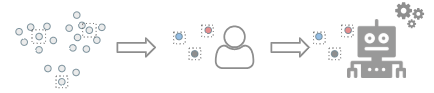
\includegraphics[width=.9\textwidth]{figures/Framework_processo_inicial.png}
  \caption{Etapa Inicial do Framework de Aprendizado Ativo}
  \label{fig:framework_AL_classico_etapa_inicial}
\end{figure}


No processo interativo já temos um classificador e um conjunto de amostras pré-rotuladas. Assim iniciamos da seguinte forma, conforme a figura ~\ref{fig:framework_AL_classico}: uma política Q seleciona um conjunto de amostras de U (1 e 2) para ser classificada por G (3). Essas amostras são levadas ao oráculo que aprova ou corrige a classificação de G (4). Após isso, essa amostra é incluída em T e o classificador pode ser retreinado, finalizando o ciclo (5). Esse processo pode ser repetido várias vezes até um critério de parada, como por decisão do oráculo, ou por não ter mais dados disponíveis em U, por exemplo. 


\begin{figure}
  \centering
  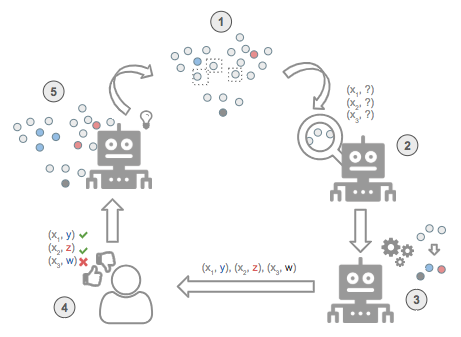
\includegraphics[width=0.9\textwidth]{figures/Framework_Active_Learning_Classico_v2.png}
  \caption{Framework Clássico de Aprendizado Ativo}
  \label{fig:framework_AL_classico}
\end{figure}


O aprendizado ativo costuma ser descrito na literatura em duas grandes etapas: i) cenários e ii) estratégia de seleção e organização das amostras [\cite{settles2014active}]. A etapa de seleção de cenários é a forma pela qual o algoritmo tem acesso aos dados. Existem diversos cenários que podem ser usados mas, independente de qual seja o escolhido, deve-se selecionar qual amostra será enviada para o oráculo através de uma função de utilidade [\cite{olsson2009literature, dasgupta2011two}]. A seguir temos a descrição detalhada dos cenários e estratégias de seleção. 


\section{Cenários do Aprendizado Ativo}
\label{sec:cenarios}

Existem diferentes cenários onde o Aprendizado Ativo poderá fazer a seleção de queries. Dentro desses, os três principais que podem ser considerados na literatura são: (i) membership query synthesis, (ii) stream-based selective sampling e (iii) pool-based sampling [\cite{settles2014active}]. A figura ~\ref{fig:ActiveLearningScenarios} abaixo sintetiza a ideia.


\begin{figure}
  \centering
  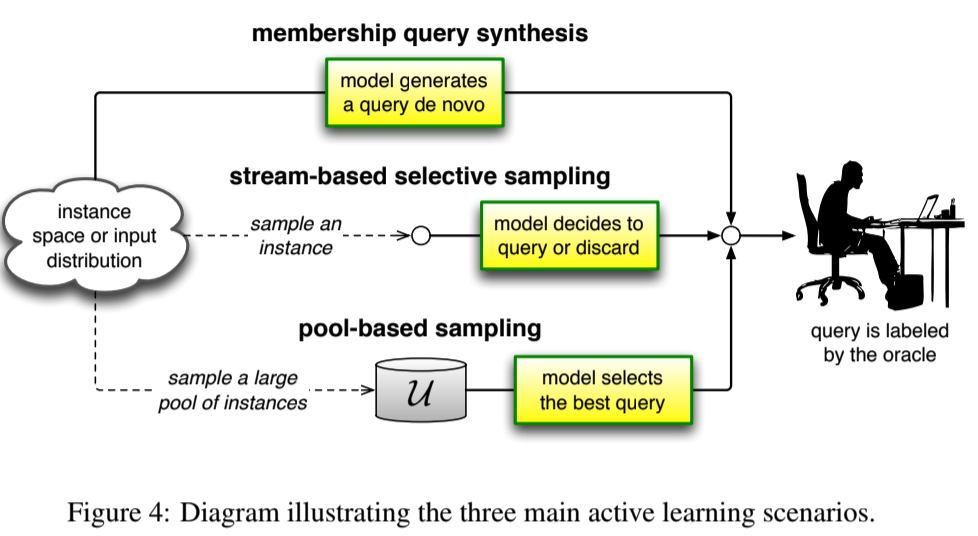
\includegraphics[width=.8\textwidth]{figures/active_learning_scenarios.png}
  \caption{Cenários de Aprendizado Ativo (Settles, 2014)}
  \label{fig:ActiveLearningScenarios}
\end{figure}


\subsection{Membership Query Synthesis}
\label{sec:cenarios_membeship}

Uma das primeiras formas de se pensar na disponibilização dos dados foi atráves do método de membership. Neste cenário, é proposto que o algoritmo crie exemplos sintéticos para serem enviados ao oráculo. Os primeiros trabalhos que utilizaram essa ideia datam de 1980 [\cite{shapiro1981algorithm, shapiro1982algorithmic, shapiro198algorithmic_2}] e há muitas formas de se fazer isso. A única premissa é que o algoritmo possua uma definição dos dados (por exemplo as dimensões da imagem). Para criar novos exemplos podemos, por exemplo, mudar a estrutura de uma imagem ou retirar partes dela.

De uma forma geral o que pretende-se fazer com esse cenário é, na distribuição do espaço de features, criar exemplos representativos. O trabalho de [\cite{baum1992query}] é um bom exemplo pois tentam sintetizar uma amostra através de uma rede neural de 2 camadas. A ideia geral, neste exemplo, é que, dada duas amostras, $x_+$ e $x_-$, das classes positiva e negativa, tenha como objetivo encontrar o melhor hiperplano que as separe. Para isso, sintetiza-se uma amostra m no meio de ambas e pede ao oráculo que nomeie a respectiva classe. Se, por exemplo, a amostra sintética m pertencer a classe $x_+$, sabe-se que o hiperplano deverá estar entre as amostras m e $x_-$. A figura ~\ref{fig:LangBaum_GeometryQueryLearning} representa essa ideia. 

\begin{figure}
  \centering
  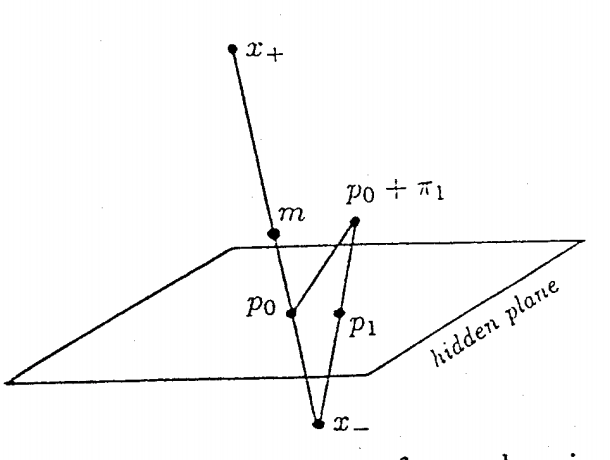
\includegraphics[width=.4\textwidth]{figures/lang_baum_geometry_query_learning.png}
  \caption{A geometria do Aprendizado por Consulta [\cite{baum1992query}]}
  \label{fig:LangBaum_GeometryQueryLearning}
\end{figure}

É importante ressaltar que há desafios nesse sentido quando temos um domínio de alta complexidade, como o caso de imagens de raio-x, por exemplo [\cite{angluin1988queries}]. Mesmo em casos que poderiam ser mais simples encontramos dificuldades. Uma das principais limitações, acontecem quando o oráculo é um humano. Na imagem ~\ref{fig:LangBaum_5vs9Example}, os autores, [\cite{baum1992query}], utilizaram da ideia acima para gerar exemplos sintéticos de imagens de números. O interessante é que, dependendo, de onde os pontos estavam dispostos, algumas imagens não possuíam nenhum significado. Inclusive, o oráculo poderia dar como resposta que determinada amostra era "não reconhecida".

\begin{figure}
  \centering
  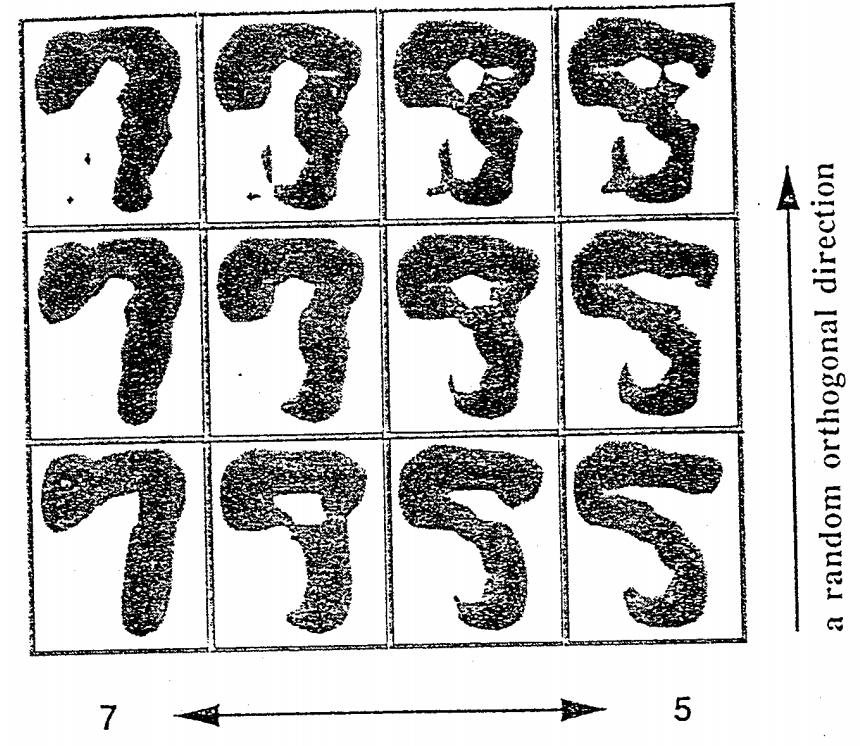
\includegraphics[width=.4\textwidth]{figures/lang_baum_5_vs_9_example.png}
  \caption{Exemplos Sintéticos sem Significado [\cite{baum1992query}]}
  \label{fig:LangBaum_5vs9Example}
\end{figure}

Apesar dessa limitação para oráculos humanos, o trabalho [\cite{king2004functional, king2009automation}] conseguiu utilizar eficientemente essa ideia para quando o oráculo é um robô. Além desse, há um trabalho que utilizou de Genrative Adversarial Networks (GAN) em conjunto com Aprendizado Ativo para criar exemplos [\cite{zhu2017generative}]. O interessante é que eles revisitaram o trabalho de Lang e Baum e conseguiram criar exemplos significativos no caso de dígitos, conforme ilustrado na figura ~\ref{fig:GAN_5_vs_9}. Entretanto, geraram amostras sem significado para fotos de cães e gatos. 

\begin{figure}
  \centering
  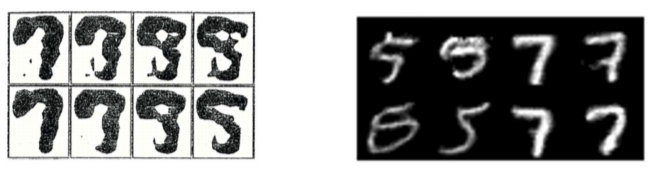
\includegraphics[width=.9\textwidth]{figures/generative_GAN_AL_5_vs_9.png}
  \caption{Esquerda: exemplo de \cite{baum1992query} revisitado e na foto à direita o exemplo gerado pela GAN. [\cite{zhu2017generative}]}
  \label{fig:GAN_5_vs_9}
\end{figure}


Há, ainda, outras iniciativas com esse cenário. No trabalho de [\cite{wang2015active}], por exemplo, utiliza-se o paradigma de criar exemplos sintéticos mas, ao final, utiliza-se exemplos da própria base de dados para serem enviados ao oráculo. Para isso seleciona-se um par de amostras {$x_+$, $x_-$} que estão separadas por um hiperplano e, então, sintetiza-se uma amostra que estará posicionada no meio, adicionada por um pequeno vetor ortogonal. A partir desta amostra sintética, seleciona-se o vizinho mais próximo que será apresentado para o oráculo. O fato de se adicionar um vetor no ponto do meio é para que as amostras sintéticas não fiquem tão concentradas na borda do hiperplano, mas estejam dispersas em torno dele. Além disso, os autores escolheram, a partir da amostra sintética, selecionar o vizinho mais próximo pois ele poderia ser reconhecido por um humano. A figura ~\ref{fig:wang_2015_membership}  mostra essa ideia. O ponto 1, por exemplo, foi criado a partir das amostras $x_+$ e $x_-$. A próxima etapa seria encontrar o vizinho mais próximo de outro par de pontos.

\begin{figure}
  \centering
  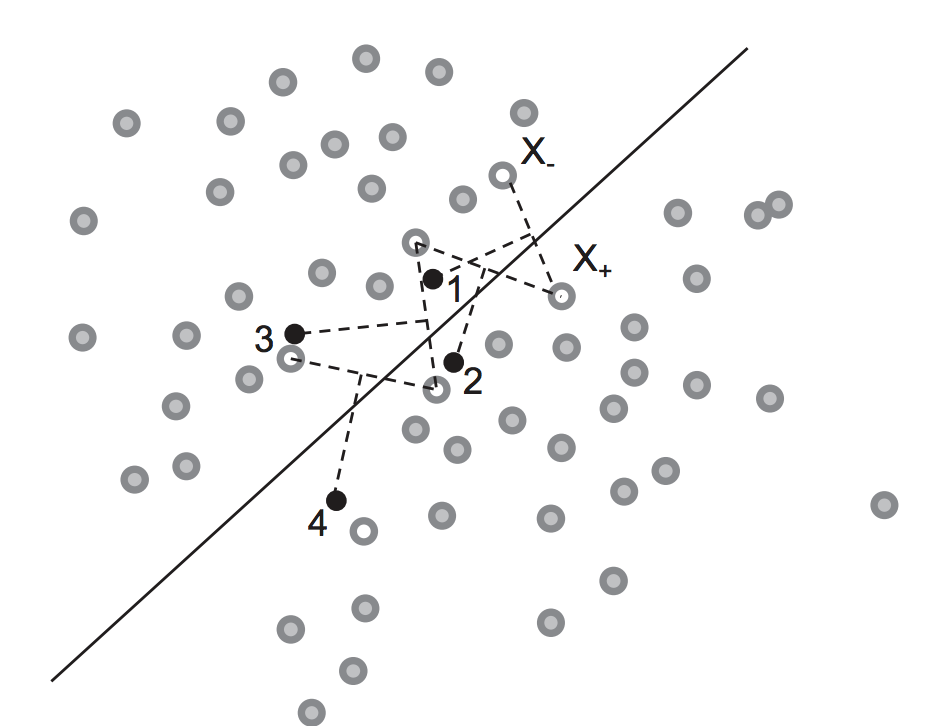
\includegraphics[width=.5\textwidth]{figures/wang_2015_membership.png}
  \caption{Exemplos representativos a partir da posição de amostras sintéticas [\cite{wang2015active}].}
  \label{fig:wang_2015_membership}
\end{figure}


\subsection{Stream-based Selective Sampling}
\label{sec:cenarios_selective_sampling}

Neste cenário permanece a premissa de que obter amostras possui um baixo custo. No entanto, as amostras são sequencialmente disponibilizadas e, através de alguma medida quantitativa, seleciona-se determinada amostra para ser levada ao oráculo ou, então, ser descartada [\cite{settles2014active}]. A figura ~\ref{fig:settles_2014_selective_sampling} mostra o fluxo. 

\begin{figure}
  \centering
  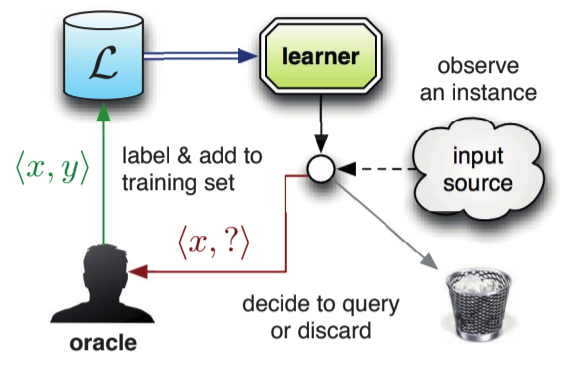
\includegraphics[width=.5\textwidth]{figures/settles_2014_selective_sampling.png}
  \caption{Fluxo do cenário de Selective Sampling [\cite{settles2014active}].}
  \label{fig:settles_2014_selective_sampling}
\end{figure}


Há algumas situações específicas pelas quais é interessante utilizar o cenário sequencial de amostras. A mais comum é quando temos, por exemplo, uma limitação no poder computacional ou de memória. Nesses casos torna-se inviável processar o conjunto de dados sem rotulação de uma única vez. Outro exemplo interessante é quando temos aplicações na web. Nesses casos, também chamado de Online Learning, é interessante que as amostras sejam escolhidas de maneira sequencial. O trabalho de [\cite{chu2011unbiased}], motivado pelos milhões de dados diários do Yahoo, mostra como esse cenário pode ser benéfico. 




\subsection{Pool-based Sampling}
\label{sec:cenarios_pool}

Dos três cenários conhecidos na literatura, o pool-based é o mais utilizado em casos reais, enquantos os anteriores são mais comuns em trabalhos teóricos. Diferentemente do cenário de selective sampling, onde uma das motivações era a falta de recursos, como poder computacional ou memória, aqui escolhemos, de inicio, todo o conjunto de dados. Assume-se, neste caso, que tenhamos um conjunto muito grande de dados sem rótulos e um pequeno conjunto de amostras rotuladas. Também temos que esse conjunto seja estático, embora isso não seja estritamente necessário. A maior diferença entre os dois é que enquanto o primeiro escolhe as amostras sequencialmente e, então, decide, o pool-based analisa todas as amostras e, baseado em uma medida de relevância, seleciona as amostras [\cite{settles2014active}]. A imagem ~\ref{fig:settles_2014_pool}  demostra o fluxo.

\begin{figure}
  \centering
  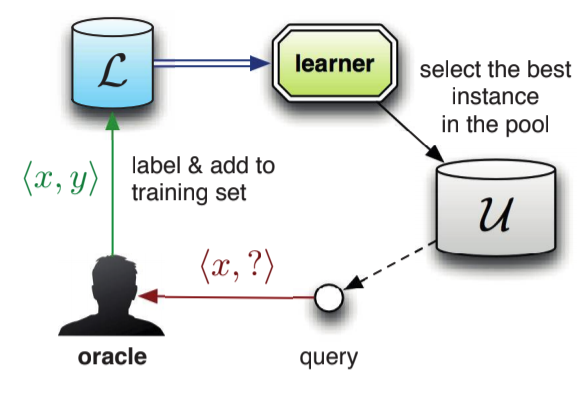
\includegraphics[width=.5\textwidth]{figures/settles_2014_pool.png}
  \caption{Fluxo do cenário de Pool-Based Sampling [\cite{settles2014active}].}
  \label{fig:settles_2014_pool}
\end{figure}

%Existem muitos trabalhos recentes que utilizam esse cenário. Por exemplo: \todo{citar trabalhos}



\section{Estratégia de Seleção e Organização das Amostras}
\label{sec:query_strategy}

Todos os cenários de Aprendizado Ativo discutidos anteriormente envolvem avaliar a relevância das amostras a serem selecionadas. Na literatura, há muitas estratégias formuladas para se fazer isso e, a seguir, temos as principais delas [\cite{settles2012active}]. É importante notar que em todas as estratégias teremos alguma medida quantificável para selecionar as amostras. Por vezes podemos ter estratégias diferentes que utilizam medidas iguais ou similares.




\subsection{Amostras Incertas} %uncertainty sampling 
\label{sec:amostras_incertas}

Amostras Incertas é uma das estratégias mais utilizadas em Aprendizado Ativo. Isso acontece provavelmente por ser muito intuitiva e de fácil implementação [\cite{settles2014active}]. A ideia básica é que precisamos encontrar exemplos que, por terem um alto grau de incerteza, serão os mais relevantes. Ou seja, queremos descartar exemplos nos quais o classificador já possui uma alta confiança de acerto e focar nos exemplos mais incertos.  


\begin{figure}
  \centering
  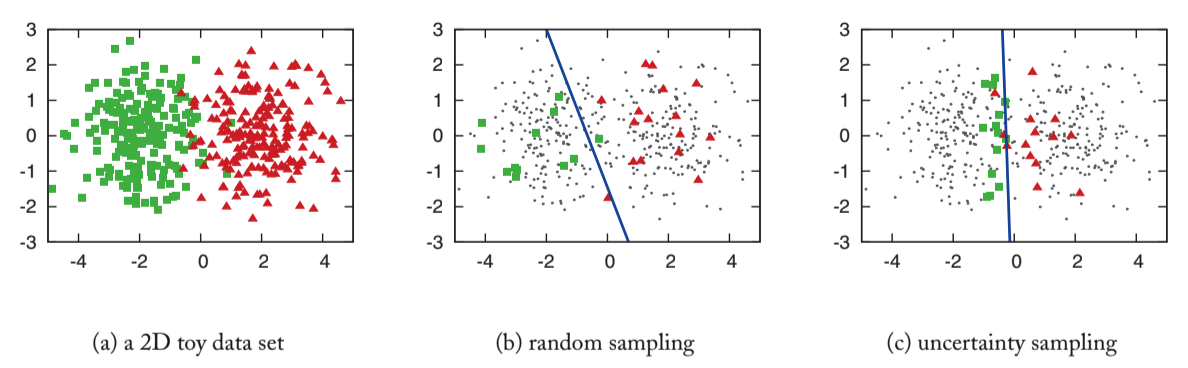
\includegraphics[width=1.0\textwidth]{figures/settles_2014_uncertainty_sampling_example.png}
  \caption{Exemplo de Amostras Incertas [\cite{settles2014active}].}
  \label{fig:settles_2014_uncertainty_example}
\end{figure}

A figura ~\ref{fig:settles_2014_uncertainty_example} exemplifica bem a ideia exposta. Nela temos como classificador uma regressão logística treinada em (b) por 30 amostras aleatórias e em (c) por 30 amostras mais relevantes. É perceptível que, comparando as duas imagens (a) e (b), o classificador obtido através das amostras incertas é o melhor. Isso ocorre porque as amostras mais relevantes estarão, nesse caso, próximas da linha vertical que separa os dois grupos de dados.

Apesar da ideia ser intuitiva precisamos encontrar uma forma de medir a incerteza das amostras. É importante notar que uma interpretação probabilística pode ajudar. Isso porque, quando colocamos nesse escopo, conseguimos generalizar e modelar essa ideia para uma enorme quantidade de casos. Sendo o $x^*_{A}$ a melhor consulta possível utilizando a medida $A$, podemos pontuar as três principais formas de medir a incerteza de uma amostra, que serão expostas abaixo [\cite{settles2014active}].


\textbf{Menos Confiante:} nessa forma estamos interessados nos exemplos nos quais temos menos certeza sobre seu rótulo.
\begin{align*}
\textbf{X}^*_{LC} = &\arg\min_{x} P_{\theta}  (\hat{y}\lvert x)\\
& = \arg\max_{x} 1 - P_{\theta}  (\hat{y}\lvert x),\\
\end{align*}

onde, $\hat{y} = \arg\max_{y} P_{\theta} (y\lvert x)$ e x representa as amostras do dataset, com x $\in$ $\mathbb{R}^n$, e que podem ser classificadas com diferentes classes, y $\in$ \{0, 1, ..., c\}. Assim, para cada x, o $\hat{y}$ é a maior probabilidade que determinada amostra tem de ser rotulada. O que a formula acima faz é olhar a probabilidade condicional na qual, em todos as possíveis amostras, possuirá o menor $\hat{y}$. Desta forma estamos selecionando as amostras mais relevantes para o framework.


Para ilustrar melhor essa ideia, suponha um exemplo onde para cada x $\in$ $\mathbb{R}^n$, temos um $\hat{y}$ de maior probabilidade. Considere um exemplo onde temos duas classes possíveis, y = [0,1]. Uma amostra qualquer $x_q$ terá, portanto, duas probabilidades condicionais para seu $\hat{y}$: P($y_0 \lvert x_q$) e P($y_1 \lvert x_q$). Como o interesse é maximizar a função, escolheremos o $\hat{y}$ de maior probabilidade. A partir disso teremos um conjunto de amostras de X com seus respectivos $\hat{y}$ e escolhemos, entre eles, a amostra mais relevante, isto é, que possui a menor probabilidade. A desvantagem dessa abordagem é que ela considera apenas a informação da melhor predição.  


\textbf{Margem:} similar a medida anterior, a margem tenta resolver a limitação de olhar apenas a melhor predição e utiliza da primeira e segunda maiores probabilidades. 


\begin{align*}
\textbf{X}^*_{M} = &\arg\min_{x}[ P_{\theta} (\hat{y_{1}}\lvert x) - P_{\theta} (\hat{y_{2}}\lvert x)]\\
&\arg\max_{x}[ P_{\theta} (\hat{y_{2}}\lvert x) - P_{\theta} (\hat{y_{1}}\lvert x)]\\
\end{align*}

Intuitivamente, para determinada amostra, caso a margem fique muito alta, significa que o classificador possui uma alta probabilidade em relação à primeira das duas maiores predições possíveis. Ao contrário, caso a margem fique estreita, o classificador não sabe ao certo qual das duas possibilidades determinada classe pertence. Suponha por exemplo que as maiores probabilidades são 0.55 e 0.40, resultando em 0.15. É difícil ter certeza qual das duas são mais relevantes para o framework. Ao contrário, suponha o exemplo onde sejam 0.90 e 0.02, resultando em 0.88. Nesse caso a probabilidade que seja a primeira amostra é muito alta em relação a segunda. Essa abordagem é interessante pois considera informações adicionais para selecionar as amostras. Entretanto, caso tenhamos um número alto de possibilidades, essa abordagem ainda não olha para toda a distribuição possível dos dados.

\textbf{Entropia:} a medida mais geral e comum leva em consideração todas as probabilidades condicionais que uma amostra pode ser classificada. Isto é, tem-se uma probabilidade condicional para cada x, $P(y\lvert x)$, e uma respectiva classe, y$\in$Y. A partir disso calcula-se a entropia H.

\begin{align*}
\textbf{X}^*_{H} = &\arg\max_{x} H_{\theta}  (Y\lvert x)\\
&\arg\max_{x} \sum_{y} P_{\theta}  (y\lvert x) \log_{} P_{\theta}  (y\lvert x),\\
\end{align*}

onde y engloba todas as possíveis classes para cada x. A entropia é máxima quando $P(y\lvert x)$ é uniforme. Dessa forma estamos olhando para todo o conjunto de possibilidades e selecionando as amostras mais incertas.


\begin{figure}
  \centering
  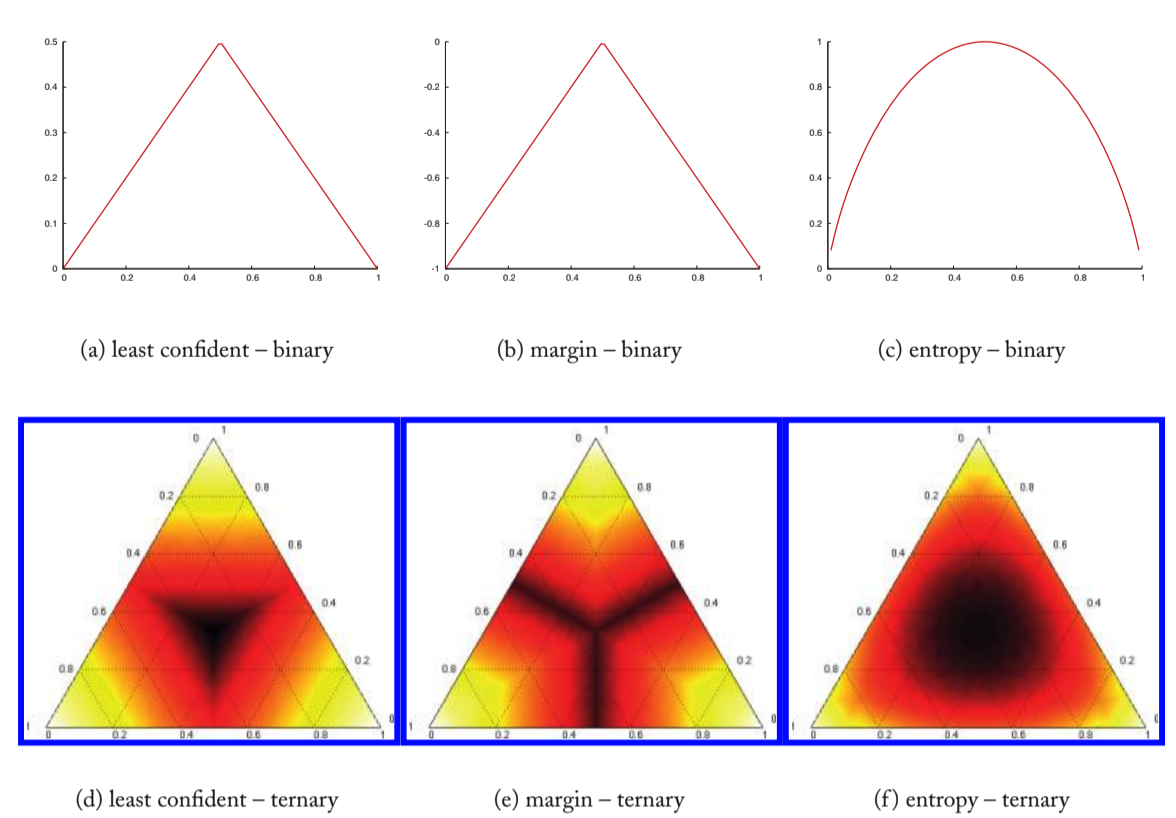
\includegraphics[width=0.8\textwidth]{figures/settles_2014_uncertainty_medidas.png}
  \caption{Comparação entre as três medidas [\cite{settles2014active}].}
  \label{fig:settles_2014_uncertainty_medidas}
\end{figure}



Uma forma de comparar as três medidas pode ser vista na figura ~\ref{fig:settles_2014_uncertainty_medidas}. Nela é possível ver o resultado das funções de relevância em termos da função da probabilidade condicional de determinada classificação, $P(y\lvert x)$. Assim, a parte superior da figura mostra, em um exemplo de classificação binária, que quando a probabilidade da classificação for 0.5, teremos o resultado de maior relevância, pois essa seria a amostra mais incerta. Da mesma forma, na parte inferior, em um exemplo com três possíveis classificações, percebemos a mesma coisa. 


\subsection{Espaço de Hipóteses} 
\label{sec:hypothesis_space}

Uma outra estratégia que pode ser utilizada é procurar amostras dentro do espaço de hipóteses [\cite{mitchell1978version, mitchell1982generalization}]. Nessa estratégia trabalharemos, por exemplo, com mais de um classificador ou com configurações diferentes de um mesmo classificador. Essa ideia foi implementada no trabalho de [\cite{atlas1990training,cohn1994improving}] e pode ser vista na figura ~\ref{fig:cohn_1994_hypothesis_space_example}. Nela temos dois tipos de classificações (0 ou 1) e quatro hipóteses diferentes. As áreas mais escuras, onde há a interseção das diferentes hipóteses, representam a região onde podem haver as amostras mais incertas. 

\begin{figure}
  \centering
  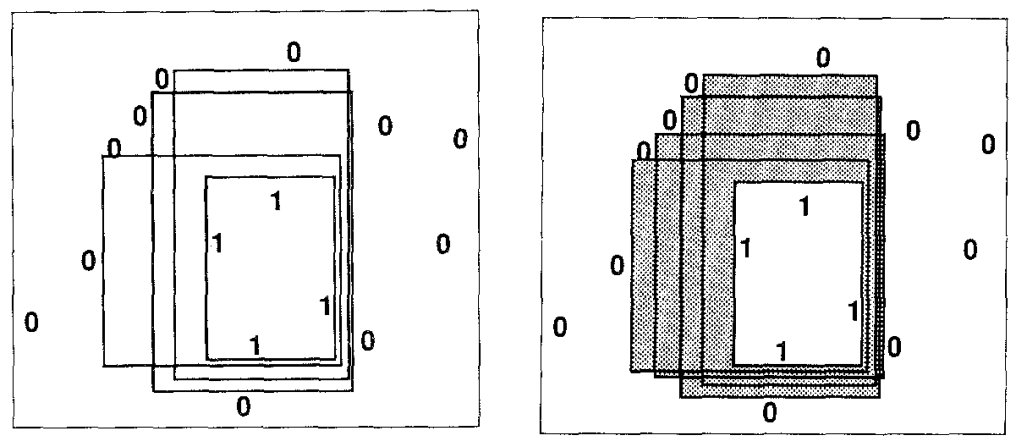
\includegraphics[width=0.7\textwidth]{figures/cohn_1994_hypothesis_space_example.png}
  \caption{Exemplo Espaço de Hipóteses [\cite{cohn1994improving}].}
  \label{fig:cohn_1994_hypothesis_space_example}
\end{figure}

Um outro exemplo mais canônico pode ser visto no trabalho de [\cite{dasgupta2011two}], no qual temos quatro classificadores lineares e a região em rosa representa a área de incerteza. Nessa estratégia uma amostra só iria ser selecionada se estivesse nessa região.

\begin{figure}
  \centering
  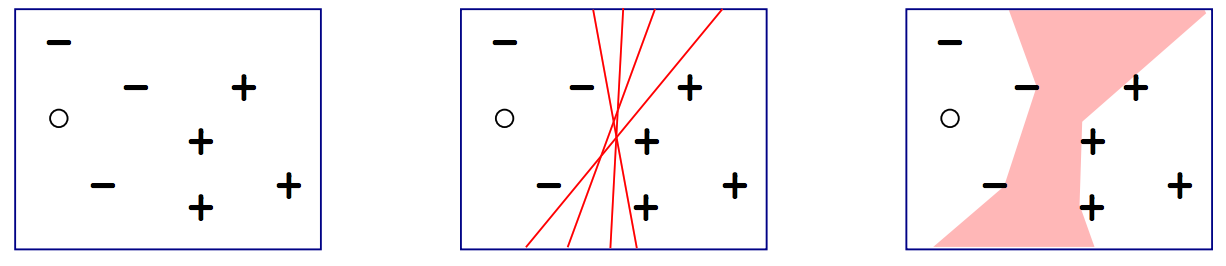
\includegraphics[width=0.9\textwidth]{figures/dasgupta_two_faces_hypothesis_example.png}
  \caption{Exemplo Espaço de Hipóteses [\cite{dasgupta2011two}].}
  \label{fig:dasgupta_two_faces_hypothesis_example}
\end{figure}


A principal forma de procurar amostras dentro do espaço de hipóteses se dá através de consultas por comitês [\cite{seung1992query}]. De uma forma geral, a ideia é que tenhamos um comitê de duas ou mais hipóteses iniciais e, em cada interação onde uma amostra é selecionada, tem-se alguma heurística para mensurar o desacordo entre elas. É importante notar que se o espaço de hipóteses for bem definido e os dados livres de ruído é possível escolher randomicamente um número de hipóteses e usar algum método para estimar o desacordo. Para os casos em que isso não é possível, a literatura apresenta muitas formas de resolver a questão, como uma abordagem bayesiana ou um ensemble de modelos. Não existe uma regra para o número de hipóteses a serem escolhidos. A literatura mostra como comum algo entre cinco a quinze hipóteses, mas pode funcionar bem com duas ou três também [\cite{settles2014active}]. 


Assim como ocorre na estratégia anterior, é necessário que tenhamos como medir a incerteza entre as diversas hipóteses. Existe uma variedade de formas de se fazer isso, mas uma das mais comuns é uma generalização da formula anterior de amostras incertas utilizando a entropia.

\textbf{Entropia por Voto:} a abordagem sugerida por [\cite{dagan1995committee}] considera todas os possíveis rótulos e o número de votos recebidos no comitê. 

\begin{align*}
\textbf{X}^*_{SVE} = - &\arg\max_{x} \sum_{y} P_{C}  (y\lvert x) \log_{} P_{C}  (y\lvert x),\\
\end{align*}

onde y contempla todos as possíveis classes, C é o número de hipóteses e $P_{C}  (y\lvert x) = \frac{1}{|C|}  \sum_{\theta \in C} P_{\theta}  (y\lvert x)$ é a média ou o consenso com maior probabilidade que y está correto, de acordo com o comitê. Novamente a vantagem de utilizar a entropia é que considera-se todas as possíveis classes em todas as possíveis hipóteses, selecionando a amostra de maior relevância.


\subsection{Amostras Incertas vs. Espaço de Hipóteses} 
\label{sec:minimizing_expected}

Uma das limitações das Amostras Incertas está no fato de que, como trabalha-se com uma região específica de dados, é possível que ocorra um processo de aprendizado míope, uma vez que foca-se em uma região particular de dados.  [\cite{settles2014active}]. A parte superior da figura ~\ref{fig:limitations_incertas} ajuda a exemplificar esse problema e a comparação com o espaço de hipóteses. Nela temos (a) o output desejado, (b) alguns dados selecionados de forma randômica, (c) uma rede neural que fez 100 interações de forma randômica, (d) 100 interações utilizando a técnica de amostras incertas e, por último, (e)100 interações utilizando o espaço de hipóteses. É perceptível que o classificador treinado com dados randômicos (c) gerou uma imagem muito distante do output verdadeiro, enquanto o espaço de hipóteses (e) é muito mais próximo dos dois triângulos (a). Além disso, apesar das amostras incertezas (d) lembrarem algo próximo a dois triângulos, continua sendo inferior ao espaço de hipóteses. É interessante notar também a evolução dos classificadores, respectivamente para 20, 40, 60, 80 e 100 interações através da técnica de espaço de hipóteses (fileira do meio da figura) e pelas amostras incertezas (parte inferior da figura).

\begin{figure}
  \centering
  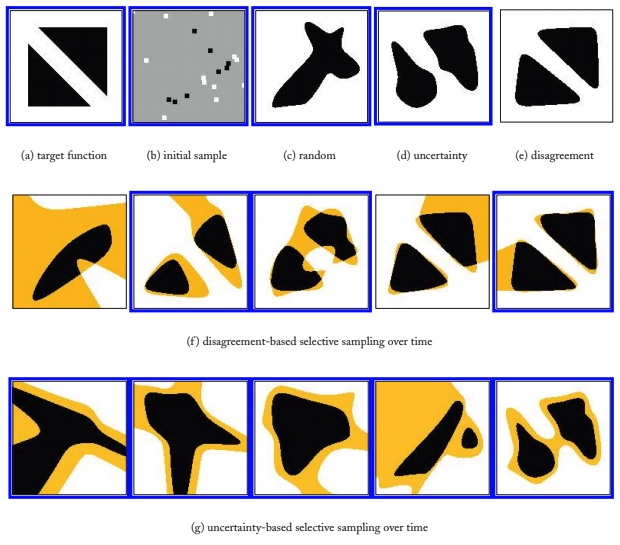
\includegraphics[width=0.7\textwidth]{figures/limitations_incertas.png}
  \caption{Limitações Amostras Incertas [\cite{settles2014active}].}
  \label{fig:limitations_incertas}
\end{figure}

Uma outra limitação, tanto das Amostras Incertas quanto do Espaço de Hipóteses, está no fato de que elas são muito sensíveis a outliers. Isso ocorre porque, nas duas estratégias, as amostras são medidas individualmente [\cite{settles2014active}]. Ou seja, não é levado em consideração a distribuição delas. A figura ~\ref{fig:limitations_outliers} ajuda a sintetizar esse caso. Nela o exemplo A seria o escolhido pois está exatamente na linha de divisão entre as duas classes. Entretanto, por ser um outlier, não é um exemplo realmente relevante. 


\begin{figure}
  \centering
  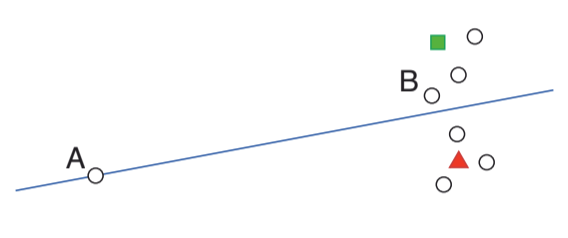
\includegraphics[width=0.5\textwidth]{figures/limitations_outliers.png}
  \caption{Limitações napresença de Outliers [\cite{settles2014active}].}
  \label{fig:limitations_outliers}
\end{figure}

 \subsection{Explorando a Estrutura dos Dados} 
\label{sec:explorando_estrutura_dados }

Uma das maneiras encontradas para resolver a limitação dos outliers é explorar a estrutura dos dados. Uma das formas interessantes de se fazer isso é utilizando a intersecção do Aprendizado Ativo com o Aprendizado Semi-Supervisionado. Podemos, por exemplo, encontrar clusters através de alguma medida de similaridade e utilizar essa informação estrutural. [\cite{saito2014active, dasgupta2011two}]. Selecionamos os centroides e pedimos para o oráculo categorizar corretamente, iniciando, assim, o ciclo do aprendizado ativo. 

Há, porém, alguns problemas na estratégia pois não temos um número óbvio de clusters. Também podemos ter vários níveis de granularidade e, o pior dos casos, os clusters podem não representar as categorias corretas do dataset [\cite{dasgupta2011two, settles2014active}].  A figura ~\ref{fig:toy_example_clustering} exemplifica essa ideia. A imagem (a) mostra uma distribuição de dados de um espaço de features. Como não temos a informação a respeito das verdadeiras classes desses dados, se aplicarmos um algoritmo não supervisionado para encontrar possíveis padrões e clusters, pode ser difícil saber quantos clusters realmente existem. Algumas possibilidades estão nas figuras b-e, mas isso não significa que representam as classes corretas desse conjunto de dados. 


\begin{figure}
  \centering
  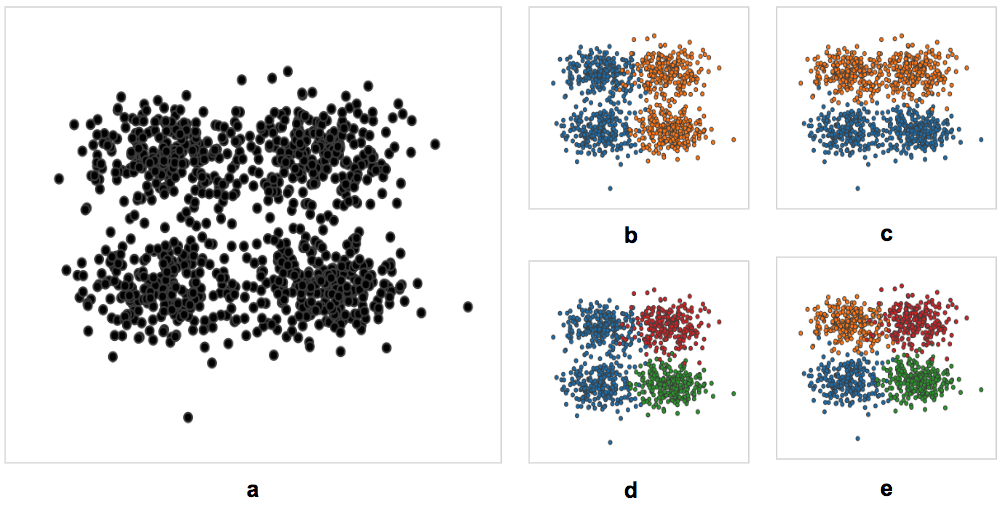
\includegraphics[width=0.9\textwidth]{figures/toy_example_clustering.png}
  \caption{Exemplo de Clustering.}
  \label{fig:toy_example_clustering}
\end{figure}


\section{Aprendizado Ativo com Participação Ativa do Usuário}
\label{sec:aprendizado_ativo_variacoes}

O aprendizado ativo tem como principal objetivo diminuir o esforço gasto na rotulação de amostras e ao mesmo tempo obter um bom classificador. Há outras técnicas que são correlatas a essa ideia, como o aprendizado semi-supervisionado [\cite{zhu2006semi}], que utiliza da própria estrutura dos dados para re-treinar o classificador. Outra técnica interessante é o transfer learning [\cite{rodrigues2018evaluation}], que tem como objetivo passar um conhecimento prévio de um problema já resolvido para algum outro similar. Além desses que foram citados podem existir diversas variações. A diferença básica é que no aprendizado ativo temos a interação de um oráculo, sendo na maioria das vezes um humano. 


Apesar dessa ideia ser muito interessante, principalmente quando temos um domínio que requer profissionais extremamente especializados para categorizar as amostras, o oráculo no framework clássico ainda é utilizado de forma muito limitada [\cite{seifert2010user}]. Nele o papel do oráculo se restringe em aceitar/corrigir as classes dadas pelo classificador. Trabalhos mais recentes vem buscando dar ao oráculo outros papéis. Na realidade, existe um grande interesse em como incorporar mais conhecimento humano dentro dessa estrutura [\cite{settles2014active}]. 

O trabalho de [\cite{castro2009human}] foi um dos primeiros a tentar relacionar, de forma quantitativa, o aprendizado ativo com a ciência cognitiva. Nesse caso o problema era conseguir identificar duas classes de ovos alienígenas que se diferenciavam pela forma. O estudo foi feito com 33 participantes através de três testes: i) aprendizado humano-ativo, ii) aprendizado computador-ativo e iii) randômico. Para cada um dos testes também foi adicionado ruído nos dados. O estudo demonstrou que o aprendizado ativo, tanto com os humanos participando da seleção e correção das classes quanto do aprendizado ativo clássico, é melhor que a forma randômica. Além disso, o aprendizado ativo, com pouco ruído nos dados, é apenas um pouco inferior ao clássico mas, a medida que dados ruidosos foram adicionados, a acurácia diminuiu, conforme mostra a figura ~\ref{fig:human_active_learning_graph}. Um outro estudo parecido feito por [\cite{markant2014better}] mostrou que, para determinados casos, o resultado é semelhante.

\begin{figure}
  \centering
  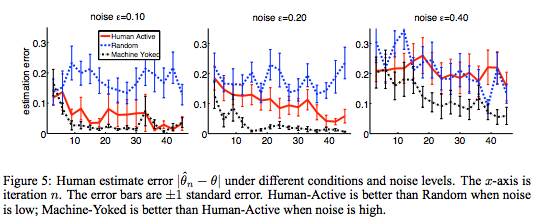
\includegraphics[width=0.9\textwidth]{figures/human_active_learning_graph.png}
  \caption{Exemplo do Estudo feito por Castro et all.}
  \label{fig:human_active_learning_graph}
\end{figure}


%% falar do Castro que eeles querem implementar em casos reais!!!

Um segundo trabalho importante de 2010 foi o de [\cite{seifert2010user}] que também buscou dar ao usuário um papel mais ativo em relação a escolha de amostras. Na pesquisa foi sugerido uma forma de visualizar o espaço de característica dos dados, conforme a o quadro esquerdo da figura ~\ref{fig:seifert_example}. As classes foram dispostas de forma igual em torno do perímetro do circulo. As regiões mais distantes do centro eram consideradas mais certas de serem classificadas com determinado rótulo. Como não foi possível fazer testes com humanos no dataset final, foi feito um experimento anterior com usuários para identificar padrões nos quais os usuários selecionavam amostras. A partir disso foi proposto dois modelos de simulação: i) modelo gaussiano e ii) modelo por convex-hull, conforme o quadro do meio e da direita da figura ~\ref{fig:seifert_example}. Ambos modelos tem como premissa que o usuário seleciona as amostras mais incertas. O primeiro estima que elas estejam no meio, pois é a região de mais incerteza. A diferença para o segundo é que ele também leva em consideração a distribuição dos dados. Os resultados mostraram que um papel ativo do usuário foi superior que o aprendizado ativo clássico para todos os casos e que nunca foi inferior às amostras randômicas, apesar de ter apresentado resultados bem próximos. Um outro ponto interessante da conclusão do estudo é que isso pode variar dependendo da base de dados e do classificador utilizado.

\begin{figure}
  \centering
  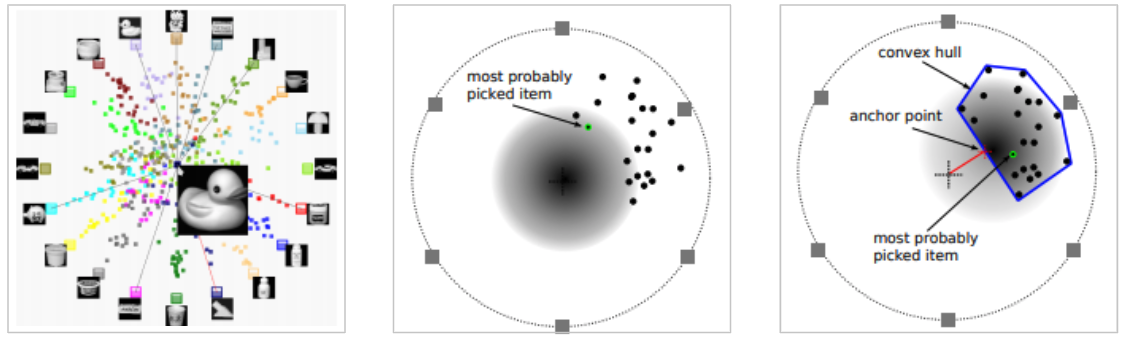
\includegraphics[width=1.0\textwidth]{figures/seifert_example.png}
  \caption{Exemplo do Estudo feito por Seifert e Granitzer.}
  \label{fig:seifert_example}
\end{figure}

O interesse em unir o conhecimento humano, incorporando-o no loop de aprendizado, continua em aberto [\cite{calma2016active}], sendo apoiado por pesquisas da área da psicologia [\cite{sim2015children}]. Um estudo recente [\cite{kottke2018other}] teve como objetivo fazer um experimento com 77 estudantes divididos em 14 grupos, dos quais nenhum deles tinha conhecimentos sobre respeito Aprendizado Computacional. O estudo comparou a acurácia dos grupos em relação à abordagem clássica do aprendizado ativo, assim como a seleção aleatória das amostras. Os resultados mostraram que, no geral, os grupos não tiveram resultados superiores em relação ao framework clássico ou em relação ao framework com amostras randômicas. Apesar disso, quando olhamos para os 5 melhores grupos, tivemos uma acurácia superior. Isso não foi determinado pelo estudo mas talvez os melhores grupos possam ser comparados com usuários experts. 

Além dos estudos abordados acima há outros dois que merecem ser mencionados, os quais analisam a interação de ferramentas visuais no processo de aprendizado ativo. Inclusive há indícios que ambas áreas estão se aproximando [\cite{sacha2016human}]. O primeiro é o trabalho do MapView [\cite{weigl2016mapview}] que propôs uma ferramenta gráfica através da redução de dimensionalidade do espaço de características para um espaço 2D. O estudo não fez comparações com a abordagem clássica de aprendizado ativo ou de amostras randômicas. Na realidade o trabalho propôs essa ferramenta e demonstrou duas principais contribuições para os usuários: i) encontrar possíveis insights em um espaço de features 2D, projetado a partir de um espaço de alta dimensionalidade e ii) através de uma abordagem visual, os usuários puderam ter um melhor entendimento do classificador. 

Um outro trabalho interessante foi o [\cite{bernard2018comparing}] no qual foi feito um estudo experimental comparando o aprendizado ativo e interações visuais. O objetivo foi descobrir se o aprendizado ativo, com uma participação ativa do usuário através de ferramentas visuais, possuía uma melhor acurácia. Além disso, buscou entender se o aprendizado ativo poderia aproveitar dessas técnicas, onde foi proposto um framework de Aprendizado Interativo Visual para rotular amostras. 

\begin{figure}
  \centering
  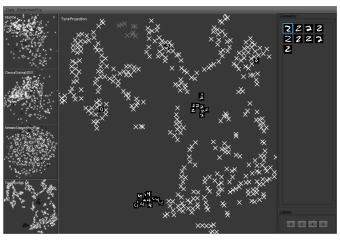
\includegraphics[width=0.8\textwidth]{figures/visual_comparing.png}
  \caption{Exemplo Ferramenta de Aprendizado Visual Interativo.}
  \label{fig:visual_comparing}
\end{figure}


O experimento foi composto por 16 pessoas, que possuíam conhecimentos prévio de análise de dados. Nele foi criado uma ferramenta visual que testou tanto a abordagem com o usuário ativo, quanto com o framework clássico. Para isso, utilizaram de algoritmos de redução de dimensionalidade e o usuário poderia escolher quais amostras ele gostaria de rotular. No framework clássico foi utilizado medidas para estimar as amostras relevantes, como foi comentado no inicio deste capítulo. A figura ~\ref{fig:visual_comparing} mostra a imagem da ferramenta visual. Os quatro pequenos quadros à esquerda representam diferentes algoritmos de redução de dimensionalidade. O usuário escolhe o de sua preferência e inicia o ciclo de escolha das amostras e rotulação. Os resultados mostraram que colocar o humano como centro do framework, com o apoio de ferramentas visuais, conseguiu competir com os modelos clássicos de aprendizado ativo. 








%  O interesse em unir o conhecimento humano, incorporando-o no loop de aprendizado, continua em aberto [\cite{calma2016active}]. Inclusive, há uma linha de pesquisa interessante que pretende fazer isso com o apoio de análises visuais, como a utilização de grafos e projeções em 2D [\cite{yang2018visually, bernard2018comparing, weigl2016mapview}]. Por exenplo, um estudo recente [\cite{kottke2018other}] teve como objetivo mudar a posição do humano de ser um especialista em categorizar amostras para ser também um especialista em selecionar. No estudo foi possível demonstrar resultados positivos, onde o aprendizado computacional pôde se beneficiar com a interação humana. 

%% comentar aqui o rtablaho do settles com NLP

%% falar quer e exclusivamente nos casos onde termos a necessidade de um especialista. Lembrar do trabalho do Baum que nao deu certo (exemplos sinteticos que nao faizam nenhum sentudo!)
\par

%% ------------------------------------------------------------------------- %%n
\chapter{Descrição da proposta}
\label{cap:Proposta}

O problema que estamos tratando, classificação de imagens de plâncton, enquadra-se na situação de dados não rotulados abundantes e com elevado custo de rotulação. Conforme mencionado na introdução, o objetivo deste trabalho é o desenvolvimento de métodos para a rotulação e classificação rápida e correta dessas imagens, a fim de que estudos posteriores, dependentes da classificação, tornem-se viáveis. 

Como foi visto no capítulo anterior, o aprendizado ativo é uma possível abordagem para rotular um grande conjunto de amostras, sem requerer a preparação prévia de um conjunto de treinamento grande. Neste processo, o usuário rotula apenas as amostras para as quais o algoritmo solicita um rótulo. De forma geral, o objetivo da abordagem é a minimização do esforço de interação do usuário. O processo continua até que uma boa taxa de classificação seja atingida. Esse classificador pode então ser utilizado para classificar novas amostras. 

Também conforme comentado no capítulo anterior, pesquisas recentes relacionadas à interação de usuários na tarefa de rotulação indicam as limitações do aprendizado ativo clássico. Nesse, o especialista tem uma atuação limitada de apenas confirmar ou corrigir o rótulo atribuído pelo algoritmo a algumas das amostras. Uma forma para contornar essas limitações são abordagens que colocam o especialista em um papel mais central, no qual sua atuação passa a incluir a possibilidade de não só corrigir ou rotular amostras selecionadas pelo algoritmo, mas também participar no processo de seleção das amostras a serem rotuladas \citep{castro2009human, kottke2018other}. Sendo que, no caso dos plânctons, estudos mostram que a incorporação de conhecimentos de especialistas aumenta a acurácia dos modelos \citep{benfield2007rapid}. A figura ~\ref{fig:frameworks_AL} demonstra essa ideia. Do lado esquerdo temos o framework já explicado nos capítulos anteriores, onde o expert participa do processo apenas para aprovar ou desaprovar a classificação feita pelo algoritmo. Do lado direito da figura, temos a mudança na etapa 2, do usuário fazendo parte das escolhas das amostras.

\begin{figure}
  \centering
  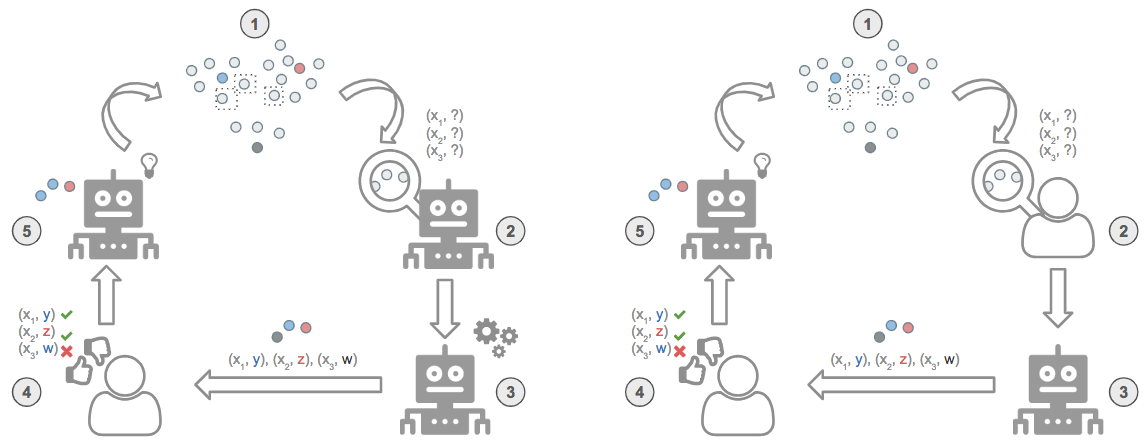
\includegraphics[width=0.9\textwidth]{figures/Frameworks_Active_Learning.png}
  \caption{esq: Framework Aprendizado Ativo Clássico, dir: Framework Aprendizado Ativo com Interação Humana na Seleção de Amostras}
  \label{fig:frameworks_AL}
\end{figure}



A proposta consiste em definirmos formas de interação do usuário, definir formas de usar a informação proveniente dessas interações, e avaliar a efetividade desse uso. Essas etapas estão descritas a seguir. Ao final descrevemos também o conjunto de dados e os procedimentos práticos que serão utilizados na parte experimental do trabalho. 



\section{Estratégia de Interação}
\label{sec:estategia_interacao}

Duas ideias de interação ativa por parte de usuários estão  sendo consideradas nesta proposta. Como elas ainda não estão suficientemente amadurecidas, é possível que a estratégia final seja uma combinação delas.

\subsection{Interação Sobre o Espaço de Projeções}
\label{sec:espaco_projecoes}

Na classificação de imagens, tipicamente são extraídas um conjunto de características das imagens e elas são utilizadas pelos classificadores. No caso de plâncton, características explicitamente extraídas em geral estão relacionados à forma e textura dos organismos. Mais recentemente, com a popularização de redes neurais profundas e, especificamente, das redes convolucionais no caso de imagens, redes pré-treinadas em outros domínios de aplicação podem ser utilizadas como extratores de características. Isto é, dada uma rede pré-treinada, passa-se uma imagem para a rede e extrai-se os valores dessa rede em alguma camada de ativação. O conjunto de valores dessa camada é utilizada como uma representação da imagem de entrada.

Sejam características extraídas explicitamente ou implicitamente, elas podem ser representadas por um vetor em $\mathbb{R}^n$. A visualização de pontos em espaços de dimensão alta não é possível. Portanto, uma técnica comumente utilizada são as projeções desses pontos sobre o espaço 2D.  

Assim como o trabalho de \citep{bernard2018comparing}, as interações dos usuários consistiriam de diferentes formas do usuário interagir com os pontos no espaço 2D.  Deve-se lembrar que cada ponto corresponde a uma imagem. Assim, durante a interação o usuário teria a possibilidade de explorar a estrutura de organização do conjunto de pontos e as imagens associadas a subconjuntos de pontos. Por exemplo, supondo que existam agrupamentos bem definidos na projeção, o usuário poderia inspecionar imagens de um desses agrupamentos e rapidamente determinar a classe predominante no grupo, excluindo apenas as que são de classes distintas. À medida que mais e mais imagens são rotuladas, esses mapas de projeção viriam também acompanhados de cores associados aos pontos já rotulados. Isto poderia ser explorado pelo usuário para rotular amostras em regiões mais críticas (presença de amostras de classes distintas).




\subsection{Interação Sobre Galeria de Imagens} 
\label{sec:galeria_imagens}

Para rotular uma imagem, o especialista precisa ver o organismo presente na imagem. Dado que estamos pressupondo uma representação  das imagens como pontos no $\mathbb{R}^n$, podemos usar métricas de similaridade para selecionar grupos de imagens similares segundo essa métrica e exibir múltiplas imagens de um grupo simultaneamente.
 
Nesta situação, supondo-se que a maior parte dos organismos são de uma mesma classe, em poucas interações o especialista pode corrigir os rótulos errados e confirmar os demais como rótulos corretos. 


\section{Uso das Informações Provenientes da Interação}
\label{sec:uso_das_informacoes_interacao}

A ideia básica do aprendizado ativo de iterar ciclos continua presente. A diferença básica é que o especialista poderá participar de forma mais ativa e selecionar as amostras a serem rotuladas.

A partir da definição de como ocorrerá essa interação, será possível também definir quais tipos de informação estarão disponíveis para o algoritmo gerar um novo classificador melhorado.



\section{Avaliação do método}
\label{sec:avaliação do método}

Propomos neste trabalho avaliar três variações do framework:
\begin{itemize}
    \item {\bf Seleção aleatória de amostras para rotulação}: esta variante é comumente utilizada como baseline quando uma nova estratégia em aprendizado ativo é desenvolvida.
    
    \item {\bf aprendizado ativo clássico}: esta é a variante na qual o oráculo tem um papel passivo de apenas confirmar ou corrigir o rótulo atribuído pelo classificador corrente. Como visto acima, diversas variações são possíveis quanto às estratégias de seleção de amostras para as consultas a serem feitas com o oráculo.
    
\item {\bf Aprendizado ativo com interação ativa de usuário:} este corresponde à variante a ser desenvolvida (oráculo ativo) neste trabalho.
\end{itemize}

O desempenho dos algoritmos é tipicamente ilustrado por meio de um gráfico "número de iterações $\times$  acurácia", que mostra como a acurácia do classificador gerado ao longo das iterações melhora com o número de iterações (exemplos podem ser vistos no capítulo~\ref{cap:Experimentos_Resultados}). O ideal é termos uma curva que atinge alta acurácia logo nas primeiras iterações. Em geral a comparação com a curva referente ao aprendizado baseado em seleção aleatória de dados é empregada para mostrar a efetividade de um algoritmo de aprendizado ativo. Esperamos portanto traçar as três curvas e a expectativa é a de que a curva referente ao aprendizado ativo com interação ativa do usuário atinja alta acurácia com um número menor de iterações.

Em um primeiro momento, as interações serão simuladas, uma vez que dispomos de datasets rotulados. Usaremos os rótulos conhecidos como sendo a resposta do oráculo. No entanto, também pretendemos fazer experimentos com usuários especialistas, como detalhado no capítulo~\ref{cap:Cronogramanotes}.

\section{Considerações sobre a parte experimental}
\label{sec:consideracoes_parte_experimental}


\subsection{Base de dados que poderão ser usados} 
\label{sec:base_usadas}

Neste trabalho teremos três bases de dados disponíveis. As especificações de cada uma estão a seguir.

\textbf{LAPS}

Este dataset foi desenvolvido pelo LAPS\footnote{LAPS: Laboratório de Sistemas Planctônicos (LAPS) do Departamento de Oceanografia Biológica, pertencente ao Instituto Oceanográfico da Universidade de São Paulo (IOUSP)} e contém 5.198 imagens de zooplanctons, divididas em 20 classes.

\textbf{NDSB}

Temos cerca de 30.000 imagens de zooplanctons, divididas em 121 classes, coletadas pelo Centro de Ciências Marinhas Hatfield da Universidade Estadual do Oregon. A fitura ~\ref{fig:ndsb} mostra alguns exemplos das imagens.

\begin{figure}
  \centering
  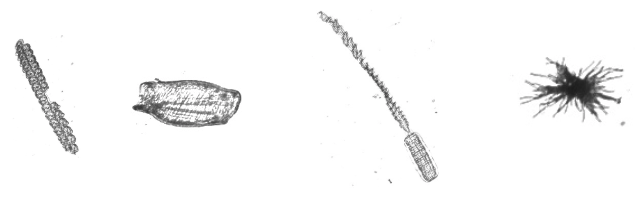
\includegraphics[width=0.9\textwidth]{figures/ndsb_exemplos.png}
  \caption{Exemplos de amostras do dataset NDSB}
  \label{fig:ndsb}
\end{figure}

\textbf{Japan}
Neste dataset temos 32.835 imagens divididas em 23 classes. A figura ~\ref{fig:japan} mostra alguns exemplos das imagens.


\begin{figure}
  \centering
  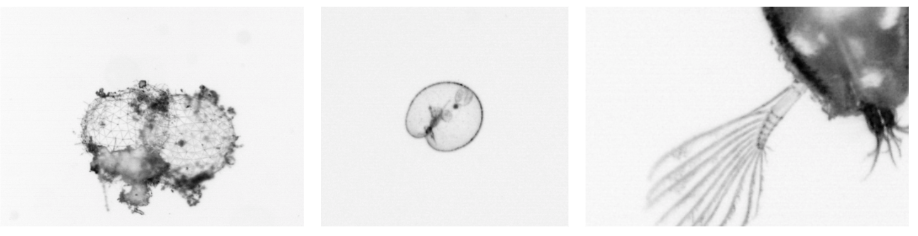
\includegraphics[width=0.9\textwidth]{figures/japan_exemplos.png}
  \caption{Exemplos de amostras do dataset Japan}
  \label{fig:japan}
\end{figure}




%\section{Extração de Features}
%\label{sec:extracao_features}

%A extração de features será feita através de uma arquitetura de Deep Learning. 


%\section{Projeção do Espaço de Features}
%\label{sec:projecao_espaco_features}

\par


%% ------------------------------------------------------------------------- %%n
\chapter{Experimentos e Resultados Preliminares}
\label{cap:Experimentos_Resultados}


Nesse capítulo serão apresentados alguns experimentos preliminares que foram feitos com dados sintéticos e com reais de Plâncton. 

\section{Framework de Aprendizado Ativo Utilizado}
\label{sec:framework_al}

O framework utilizado nesses experimentos foram baseados no trabalho de [\cite{saito2014active}]. A figura ~\ref{fig:priscila_algoritmo} e os seguintes passos explicam as etapas:

\begin{figure}
  \centering
  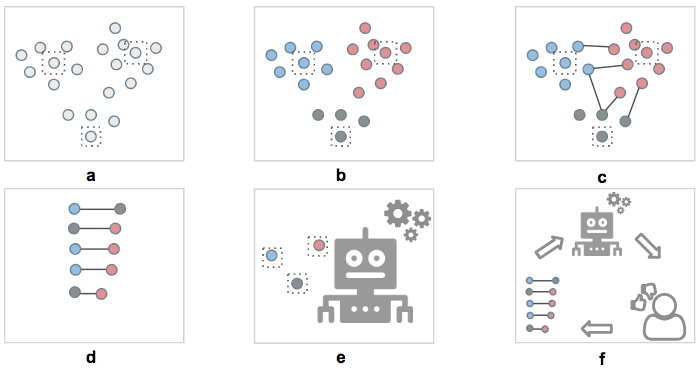
\includegraphics[width=0.8\textwidth]{figures/priscila_algoritmo.png}
  \caption{Framework Utilizado nos Experimentos}
  \label{fig:priscila_algoritmo}
\end{figure}




\begin{enumerate}
  \item No primeiro quadro (a), temos um conjunto de dados que representam um espaço de features. Inicialmente esses dados não estão rotulados, então não sabemos quais suas verdadeiras classes. Temos a informação de quantas classes podem existir para esses dados;
  \item Em (b), aplicamos um algoritmo não-supervisionado de clusterização. No nosso caso utilizamos o K-means e utilizamos como k duas vezes o número de classes possíveis;
  \item No (c), a partir do momento que temos os K-clusters, aplicamos o algoritmo de vizinhos próximos KNN para gerarmos um grafo. O número de vizinhos foi escolhido de forma prática;
  \item Em (d), reduzimos o dataset original para os dados que possuem alguma relação KNN com vizinhos que sejam diferentes da classe do seu respectivo cluster. A ideia é que tenhamos apenas os dados que estejam na borda dos cluters pois eles são mais representativos;
  \item Ainda em (d), ordenamos as amostras do dataset reduzido, de maneira decrescente, através da distância euclidiana das arestas. Iniciamos por elas pois temos como premisa que uma maior distância pode representar amostras mais relevantes;
  \item Nos quadros (e) e (f), como sabemos os rótulos verdadeiros dos dados, geramos um classificador através dos centroides dos clusters. Esses dados compõe um novo dataset que será utilizado como base de treinamento. A partir disso entramos no ciclo do Aprendizado Ativo. A cada inicio do ciclo, selecionamos n amostras do dataset reduzido e o classificador gera as previsões dos dados. Comparamos o resultado com os rótulos verdadeiros e, caso esteja incorreto, corrigimos e incorporamos esse dados para a base de treinamento. Esse ciclo continua até que os dados disponíveis no dataset reduzido acabem. 
\end{enumerate}

No caso dos dados rândomicos seguimos a mesma lógica até o passo 2. A partir disso geramos um classificador também pelos centróids a iniciamos um ciclo de aprendizado onde, a cada ciclo, selecionamos n dados, com a diferença de ser de forma rândomica.

\section{Experimentos com Dados Sintéticos}
\label{sec:experimentos_sinteticos}

Para os experimentos com dados sintéticos, geramos um dataset com 1000 amostras que representam um espaço de features 2D. A figura ~\ref{fig:exemplo_sintetico_1} mostra do lado esquerdo os dados gerados sem nenhuma classe, enquanto o lado direito mostra os rótulos verdadeiros. 


\begin{figure}
  \centering
  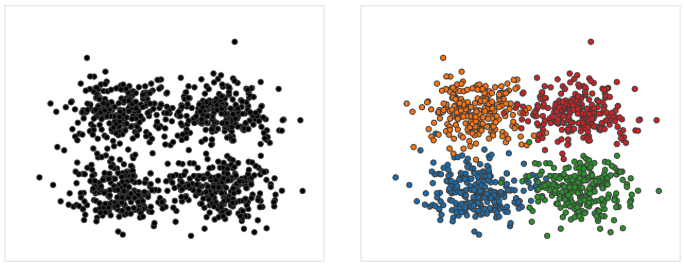
\includegraphics[width=0.9\textwidth]{figures/toy_example_1.png}
  \caption{Exemplo Sintético}
  \label{fig:exemplo_sintetico_1}
\end{figure}

Aplicamos o framework anterior neste dataset. Como temos como premissa que são quatro classes possíveis, utilizamos no K-means oito clusters. A partir disso aplicamos o algoritmo de KNN e obtemos a relações de interesse, conforme a figura ~\ref{fig:exemplo_sintetico_2}. 

\begin{figure}
  \centering
  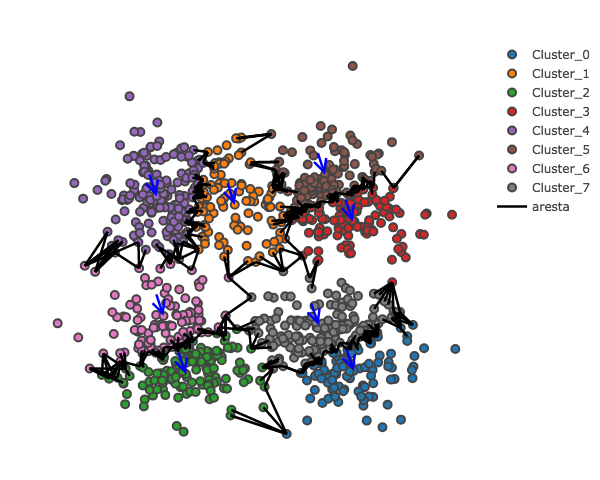
\includegraphics[width=0.8\textwidth]{figures/toy_example_2.png}
  \caption{Exemplo Sintético}
  \label{fig:exemplo_sintetico_2}
\end{figure}

É interessante notar que algumas amostras podem não ser tão relevantes pois pertencem ao mesmo grupo. Por exemplo os clusters laranja (1) e roxo (4), na imagem ~\ref{fig:exemplo_sintetico_2}, que pertencem à mesma classe. Apesar disso, como o classificador será treinado inicialmente com o centroide de cada classe, é provável que a predição convirja rapidamente. De qualquer forma, os dados mais relevantes estão entre as amostras que não são da mesma classe. 


\begin{figure}
  \centering
  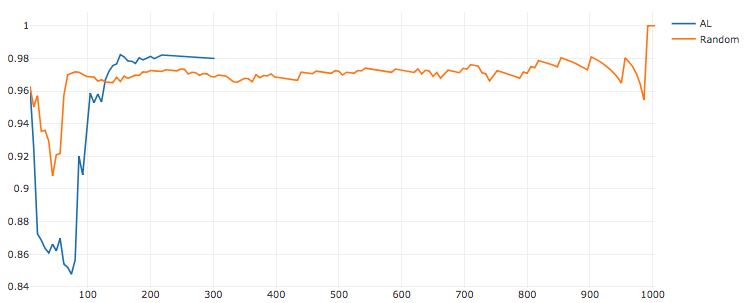
\includegraphics[width=0.9\textwidth]{figures/grafico_exemplo_sintetico.png}
  \caption{Gráfico com Resultados dos Dados Sintéticos}
  \label{fig:grafico_exemplo_sintetico}
\end{figure}

Fizemos os testes com a abordagem do Aprendizado Ativo e através de forma randômica. Escolhemos dez vizinhos próximos para encontrar as arestas e isso nos gerou um total de 300 dados, o que representa um redução de 70\% do dataset original. O gráfico ~\ref{fig:grafico_exemplo_sintetico} mostra a performance de ambos frameworks. É interessante notar que inicialmente o framework de Aprendizado Ativo não possui uma boa acurácia mas, após algumas amostras, entra numa sequência crescente, chegando em 98\% com 302 amostras, enquanto, se selecionamos os dados de forma randômica chegamos em 96.88\%. Além disso, com os dados aleatórios, atingimos um valor de 98\% apenas a partir das 900 amostras. Apesar de ambos os resultados terem uma boa taxa de acerto (provavelmente por ser um exemplo simples), o framework de Aprendizado Ativo mostrou a mesma taxa de acerto que a forma randômica com 1/3 de amostras necessárias. 


\section{Experimentos com Dados de Plâncton}
\label{sec:experimentos_plancton}

Para os experimentos com dados de Plâncton utilizamos a base de dados da FURG e escolhemos apenas 6 classes possíveis de Plâncton. A figura ~\ref{fig:Plancton_Exemplos} mostra alguns exemplos de imagens.Quando aplicado o K-means foi utilizado doze clusters, seguindo a mesma lógica de termos o dobro de clusters para o máximo esperado de classes. Para os vizinhos próximos foi utilizado o valor de 8 vizinhos. 

\begin{figure}
  \centering
  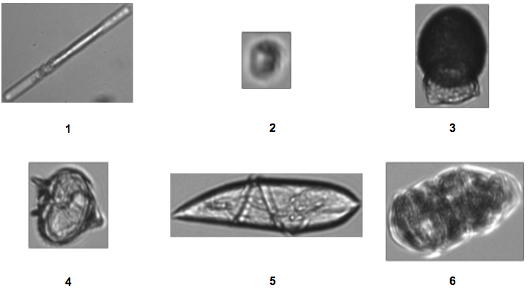
\includegraphics[width=0.6\textwidth]{figures/Plancton_Exemplos.png}
  \caption{Exemplos de Imagens de Plâncton Utilizadas. As classes são 1:Bacillariophycidae-1, 2:Prorocentrales, 3:Spirotrichea, 4:Peridiniales, 5:Gymnodiniales, 6:Cochlodinium}
  \label{fig:Plancton_Exemplos}
\end{figure}


\begin{figure}
  \centering
  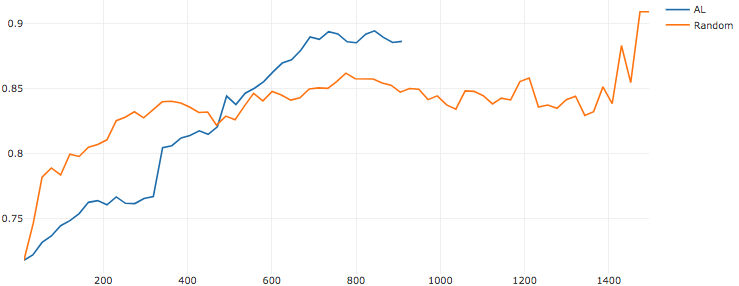
\includegraphics[width=0.9\textwidth]{figures/grafico_exemplo_plancton.png}
  \caption{Gráfico com Resultados dos Dados de Plâncton}
  \label{fig:grafico_exemplo_plancton}
\end{figure}

Assim como ocorreu com os exemplo sintético, os resultados mostraram que, nas primeiras interações, o framework de Aprendizado Ativo é inferior ao randômico mas, a partir da interação 22, com 471 dados, os dois frameworks possuem a mesma acurácia de 82\%. Desta interação em diante o Aprendizado Ativo apenas melhora sua performance, enquando os dados aleatórios permanecem em uma tendência constante. No final, com cerca de 900 amostras, o framework de Aprendizado Ativo chega em uma acurácia de 88.62\%. Os dados aleatórios só chegam nessa acurácia com cderca de 1400 amostras. Isto é, com 2/3 do esforço atingimos a mesma acurácia.
\par


%% ------------------------------------------------------------------------- %%n
\chapter{Plano de Trabalho e Cronograma}
\label{cap:Cronogramanotes}

Os créditos em disciplinas necessários para o programa de mestrado em Ciência da Computação
no IME-USP foram cumpridos de fevereiro de 2016 até junho de 2018, conforme a tabela: 

\begin{center}
\begin{tabular}{ |l|l|l| } 
\hline
\textbf{Código} & \textbf{Disciplina}                                   & \textbf{Término} \\ 
\hline
MAC5710     & Estrutura de Dados e sua Manipulação (Aluno Especial)     & 10/06/2016       \\
MAC4722     & Linguagens, Autômatos e Computabilidade                   & 30/06/2017       \\
MAC6910     & Metodologia de Pesquisa para Ciência da Computação        & 30/06/2017       \\
MAC5749     & Análise e Reconhecimento de Formas: Teoria e Prática      & 24/11/2017       \\
MAC5861     & Modelagem de Banco de Dados                               & 24/11/2017       \\
MAC5832     & Aprendizagem de Máquina: Modelos, Algoritmos e Aplicações & 22/06/2018       \\
\hline
\end{tabular}
% \label{tab:disciplinas}
\end{center}

\section{Plano de Trabalho}
\label{sec:Plano_de_Trabalho}

O plano de trabalho será composto nas seguintes tarefas:

\begin{enumerate}
  \item Estudo de trabalhos existentes com framework entre participação ativa do usuário e Aprendizado Ativo;
  \item Estudo e Implementação de diferentes frameworks de Aprendizado Ativo;
  \item Ciar ferramenta de Aprendizado Ativo com participação ativa do usuário;
  \item Fazer testes no laboratório com especialistas do Instituto de Oceanográfico da USP (IO-USO);
  \item Escrever dissertação e Defesa do Mestrado.
\end{enumerate}


\section{Cronograma}
\label{sec:cronograma}


\begin{figure}
  \centering
  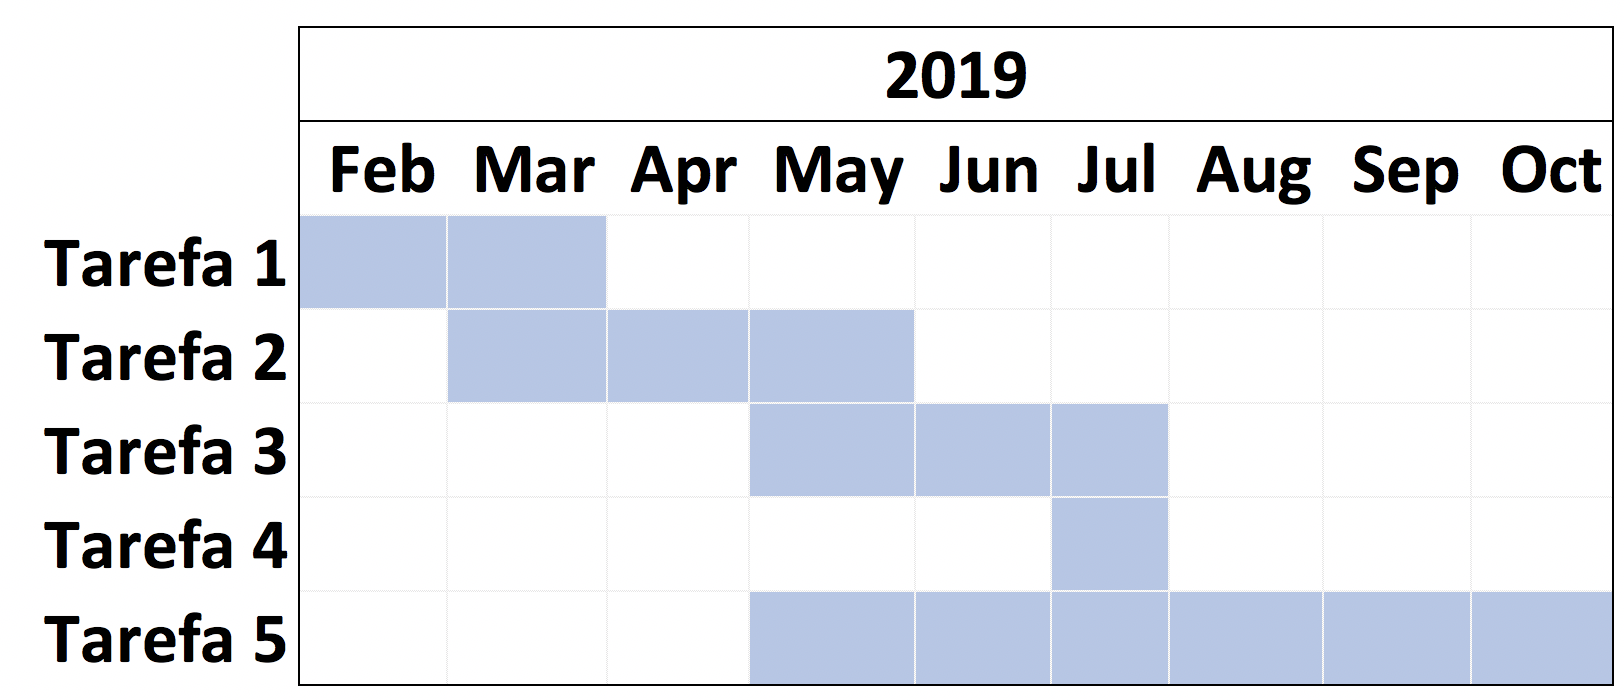
\includegraphics[width=0.4\textwidth]{figures/cronograma.png}
  \caption{Cronograma Mestrado.}
  \label{fig:cronograma}
\end{figure}

\par


%\chapter{Usando o \LaTeX{} e este modelo}

Não é necessário que o texto seja redigido usando \LaTeX{}, mas é fortemente
recomendado o uso dessa ferramenta, pois ela facilita diversas etapas do
trabalho e o resultado final é muito bom\footnote{O uso de um sistema de
controle de versões, como mercurial (\url{mercurial-scm.org}) ou git
(\url{git-scm.com}), também é altamente recomendado.}. Este modelo inclui
vários comentários explicativos e pacotes interessantes para auxiliá-lo com
ele.

O modelo é composto por estes arquivos:

\begin{itemize}
  \item Arquivo principal:
  \begin{itemize}
    \item \texttt{tese-exemplo.tex} (leia os comentários neste arquivo!)
  \end{itemize}

  \item Arquivo com as \textit{packages} usadas e suas configurações:
  \begin{itemize}
    \item \texttt{miolo-preambulo.tex} (leia os comentários neste arquivo!)
  \end{itemize}

  \item Arquivos com formato sugerido de capa, resumo e outros elementos:
  \begin{itemize}
    \item \texttt{imeusp.sty} (configurações de formatação -- não é preciso editar)
    \item \texttt{metadados-tese.tex} (é preciso inserir os metadados aqui)
    \item \texttt{folhas-de-rosto.tex} (resumo, dedicatória etc.)
  \end{itemize}

  \item Arquivos dos capítulos e apêndice:
  \begin{itemize}
    \item \texttt{cap-introducao.tex}
    \item \texttt{cap-latex.tex}
    \item \texttt{cap-tutorial.tex}
    \item \texttt{cap-exemplos.tex}
    \item \texttt{cap-conclusoes.tex}
    \item \texttt{ape-conjuntos.tex}
  \end{itemize}

  \item Diretório de figuras:
  \begin{itemize}
    \item \texttt{./figuras/}
  \end{itemize}

  \item Outros arquivos auxiliares:
  \begin{itemize}
    \item \texttt{bibliografia.bib} (arquivo de dados bibliográficos)
    \item \texttt{plainnat-ime.bbx} (estilo plainnat para bibliografias com biblatex)\index{biblatex}
    \item \texttt{plainnat-ime.cbx} (estilo plainnat para citações com biblatex)
    \item \texttt{plainnat-ime.bst} (estilo plainnat para bibliografias com bibtex)\index{bibtex}
    \item \texttt{alpha-ime.bst} (estilo alpha para bibliografias com bibtex)\index{bibtex}
    \item \texttt{natbib-ime.sty} (tradução da \textit{package} padrão natbib -- citações com bibtex)\index{natbib}
    \item \texttt{hyperxindy.xdy} (arquivo de configuração para hiperlinks no índice remissivo)
    \item \texttt{Makefile} (arquivo que automatiza a geração do documento com o comando \textsf{make})
    \item \texttt{latexmkrc} (arquivo que automatiza a geração do documento com o comando \textsf{latexmk})
  \end{itemize}
\end{itemize}

Para compilar o documento, basta executar o comando \textsf{latexmk} (ou
\textsf{make}). Talvez seu editor ofereça uma opção de menu para compilar o
documento, mas ele provavelmente depende do \textsf{latexmk} para isso.
\LaTeX{} gera diversos arquivos auxiliares durante a compilação que, em
algumas raras situações, podem ficar inconsistentes (causando erros de
compilação ou erros no PDF gerado, como referências faltando ou numeração de
páginas incorreta no sumário). Nesse caso, é só usar o comando
\textsf{latexmk -C} (ou \textsf{make clean}), que apaga todos os arquivos
auxiliares gerados, e em seguida rodar \textsf{latexmk} (ou \textsf{make})
novamente.

\section{Instalação do \LaTeX{}}

\LaTeX{} é, na verdade, um conjunto de programas. Ao invés de procurar e
baixar cada um deles, o mais comum é baixar um pacote com todos eles juntos.
Há dois pacotes desse tipo disponíveis: MiK\TeX{} (\url{miktex.org}) e
\TeX{}Live (\url{www.tug.org/texlive}). Ambos funcionam em Linux, Windows e
MacOS X. Em Linux, \TeX{}Live costuma estar disponível para instalação junto
com os demais opcionais do sistema. Em MacOS X, o mais popular é o Mac\TeX{}
(\url{www.tug.org/mactex/}), a versão do \TeX{}Live para MacOS X.  Em Windows,
o mais comumente usado é o MiK\TeX{}.

Por padrão, eles não instalam tudo que está disponível, mas sim apenas os
componentes mais usados, e oferecem um gestor de pacotes que permite adicionar
outros. Embora uma instalação completa do \LaTeX{} seja relativamente grande
(perto de 5GB), em geral vale a pena instalar a maior parte dos pacotes. Se
você preferir uma instalação mais ``enxuta'', não deixe de incluir todos os
pacotes necessários para este modelo. Por exemplo, no debian:

\begin{description}
  \item [inconsolata] -- está incluído em ``texlive-fonts-extra''
  \item [siunitx] -- está incluído em ``texlive-science''
  \item [biblatex] -- está incluído em ``texlive-bibtex-extra''
  \item [biber] -- é um pacote separado
  \item [xindy] -- é um pacote separado
\end{description}

Também é muito importante ter o \textsf{latexmk} (ou o \textsf{make}). No Linux,
a instalação é similar à de outros programas. No MacOS X e no Windows,
\textsf{latexmk} pode ser instalado pelo gestor de pacotes do MiK\TeX{} ou
\TeX{}Live. Observe que ele depende da linguagem \textsf{perl}, que precisa ser
instalada à parte no Windows (\url{www.perl.org/get.html}).

\section{Bibliografia}

Você pode usar referências bibliográficas nos formatos ``alpha'' ou ``plainnat''.
Se estiver usando natbib+bibtex\index{natbib}\index{bibtex}, use os arquivos .bst
``alpha-ime.bst'' ou ``plainnat-ime.bst'', que são versões desses dois formatos
traduzidas para o português. Se estiver usando biblatex\index{biblatex}
(recomendado), escolha o estilo ``alphabetic'' (que é um dos estilos padrão do
biblatex) ou ``plainnat-ime''. O arquivo de exemplo inclui todas essas opções;
basta des-comentar as linhas correspondentes e, se necessário, modificar o
arquivo Makefile para chamar o bibtex\index{bibtex} ao invés do
biber\index{biber} (este último é usado em conjunto com o biblatex).

\section{Perguntas Frequentes sobre o Modelo}

\begin{itemize}

\item \textbf{Posso usar pacotes \LaTeX{} adicionais aos sugeridos, como por exemplo: pstricks, pst-all, etc?}\\
Com certeza! Você pode modificar o arquivo o quanto desejar. O modelo \LaTeX{} serve só como uma ajuda inicial para o seu trabalho.

\item \textbf{As figuras podem ser colocadas no meio do texto ou devem ficar no final dos capítulos?}\\
Em geral as figuras devem ser apresentadas assim que forem referenciadas. Colocá-las no final dos capítulos dificultaria um pouco a leitura, mas isso depende do estilo do autor, orientador, ou lugar de publicação. Converse com seu orientador!

\item \textbf{Existe algo específico para citações de páginas web?}\\
Biblatex define o tipo ``online''; bibtex\index{bibtex}, por padrão, não tem um tipo específico. Se o que você está citando não é um texto específico mas sim um sítio, como por exemplo o sítio de uma empresa ou de um produto, pode ser mais adequado colocar a referência como nota de rodapé e não na lista de referências; nesses casos, algumas pessoas acrescentam uma segunda lista de referências especificamente para recursos \emph{online} (biblatex \index{biblatex} permite criar múltiplas bibliografias). Se, no entanto, trata-se de um texto específico, como uma postagem em um blog, uma matéria jornalística ou mesmo uma mensagem de email para uma lista de discussão, a citação deve seguir o formato de outros tipos de documento e informar título, autor etc. Normalmente usa-se o campo ``howpublished'' para especificar que se trata de um recurso \emph{online}. Observe também que artigos que fazem parte de uma publicação, como os anais de um congresso, e que estão disponíveis \emph{online} devem ser citados por seu tipo verdadeiro e apenas incluir o campo ``url'' (não é nem necessário usar o comando \textsf{\textbackslash{}url\{\}}), aceito por todos os tipos de documento do bibtex/biblatex.

\item \textbf{A bibliografia está sendo impressa em inglês (usa ``and'' ao invés de ``e'' para separar os nomes dos autores)}\\
Você deve estar usando um estilo de bibliografia bibtex diferente dos sugeridos. Uma simples solução é copiar o arquivo de estilo correspondente da sua instalação \LaTeX{} para o diretório onde seus arquivos estão e mudar ``and'' por ``e'' (ou ``\&'' se preferir) na função format.names. Biblatex tem pleno suporte a diferentes línguas e é possível personalizar as traduções (há um exemplo no modelo).

\item \textbf{Aparece uma folha em branco entre os capítulos}\\
Essa característica foi colocada propositalmente, dado que todo capítulo deve (ou deveria) começar em uma página de numeração ímpar (lado direito do documento). Acrescente ``openany'' como opção da classe, i.e., \textsf{\textbackslash{}documentclass[openany,11pt,twoside,a4paper]\{book\}}.

\item \textbf{É possível resumir o nome das seções/capítulos que aparece no topo das páginas?}\\
Sim, usando a sintaxe \textsf{\textbackslash{}section[mini-titulo]\{titulo enorme\}}. Isso é especialmente útil nos \textit{captions}\index{Legendas} das figuras e tabelas, que muitas vezes são demasiadamente longos para a lista de figuras/tabelas.

\item \textbf{Existe algum programa para gerenciar referências em formato bibtex?}\\
Sim, há vários. Uma opção bem comum é o JabRef; outra é usar Zotero\index{Zotero} ou Mendeley\index{Mendeley} e exportar os dados deles no formato .bib.

\item \textbf{Como faço para usar o Makefile (comando make) no Windows?}\\
Se você instalou o \LaTeX{} usando o Cygwin, você já deve ter o comando make instalado; se não, tente o MSYS2. Se você pretende usar algum dos editores sugeridos, é possível deixar a compilação a cargo deles, dispensando o uso do make.
\end{itemize}

%\par

%% Vamos definir alguns comandos auxiliares para facilitar.

% "textbackslash" é muito comprido.
\newcommand{\sla}{\textbackslash}

% Vamos escrever comandos (como "make" ou "itemize") com formatação especial.
\newcommand{\cmd}[1]{\textsf{#1}}

% Idem para packages; aqui estamos usando a mesma formatação de \cmd,
% mas poderíamos escolher outra.
\newcommand{\pkg}[1]{\textsf{#1}}

% A maioria dos comandos LaTeX começa com "\"; vamos criar um
% comando que já coloca essa barra e formata com "\cmd".
\newcommand{\ltxcmd}[1]{\cmd{\sla{}#1}}

\chapter{Do zero ao mínimo com \LaTeX{}}

Preparar um texto para impressão envolve duas coisas:

\begin{description}
\item[Escrever:] digitar, recortar/colar trechos, revisar etc.
\item[Formatar:] definir o tamanho da fonte, o
espaçamento entre parágrafos etc.
\end{description}

Hoje é comum fazer essas duas coisas ao mesmo tempo, graças à visualização
imediata que o computador oferece. No entanto, imagine como era o processo de
produção de um livro nos anos 1970: o autor escrevia seu texto em uma máquina
de escrever e enviava esse material para o editor, que era responsável pela
tarefa de formatá-lo para impressão. O autor muitas vezes inseria anotações
para o editor explicando coisas como ``este parágrafo é uma citação'', e o
editor criava algum mecanismo visual para representar isso.

Não é de se surpreender que, com o surgimento do microcomputador, os primeiros
programas para criação de textos seguissem um funcionamento similar: o autor
digitava e editava seu texto sem formatá-lo visualmente, apenas inserindo
alguns comandos correspondentes a aspectos da formatação que ele depois
revisava na versão impressa. \LaTeX{} é uma ferramenta baseada nesse processo:
você prepara seu texto no editor de sua preferência, insere comandos no texto
que indicam a estrutura do documento e o processa com o \LaTeX{}, que gera um
arquivo PDF formatado. Embora seja um estilo ``antigo'' de trabalhar, ele é
muito eficiente em vários casos. Ou seja, dependendo da situação, pode ser
mais adequado trabalhar fazendo tudo ao mesmo tempo ou dividindo o trabalho
nessas duas fases. De maneira geral:

\begin{itemize}
\item Se você precisa criar páginas diferentes entre si com \emph{layout}
definido manualmente, é melhor usar uma ferramenta que permita trabalhar
visualmente, como LibreOffice Writer, MS-Word, Google Docs etc.;

\item Se você precisa fazer um documento relativamente longo com estrutura
regular (capítulos, seções etc.), é melhor usar ferramentas que formalizam
essa estrutura (como \LaTeX{}) ao invés de usar ferramentas visuais;

\item Se você precisa fazer um documento envolvendo referências cruzadas,
bibliografia relativamente extensa ou fórmulas matemáticas, é difícil
encontrar outra ferramenta tão eficiente quanto \LaTeX{};

\item Se você precisa criar um documento simples, ambas as abordagens
funcionam bem; cada um escolhe esta ou aquela em função da familiaridade
com as ferramentas;

\item Se você quer que a qualidade tipográfica do resultado seja realmente
excelente, é necessário usar uma ferramenta profissional, como \LaTeX{},
Scribus, Adobe InDesign ou outras; processadores de texto convencionais não
oferecem o mesmo nível de qualidade dessas ferramentas.
\end{itemize}

\section{Visão Geral}

Com \LaTeX{}, você prepara o texto (incluindo as indicações de estrutura) em
um editor de textos qualquer, salva como arquivo de texto puro (``.txt'',
mas é comum usar a extensão ``.tex'' ao invés de ``.txt'') e processa esse
arquivo com o comando ``pdflatex'' (``compila'' o documento) para obter o
PDF correspondente. Qualquer editor capaz de salvar arquivos em formato
texto puro, como o bloco de notas do windows, vim, emacs etc. pode ser usado.
Programas como LibreOffice Writer, MS-Word etc. também funcionam, mas
possivelmente vão gerar dores de cabeça porque vão tentar formatar algumas
coisas automaticamente (e de maneira incompatível com \LaTeX{}).

Se você preferir, existem editores projetados especificamente para trabalhar
com \LaTeX{}; eles em geral utilizam cores para distinguir o texto dos
comandos de formatação, automatizam o processo de compilação do documento e
oferecem outras comodidades. Os mais comumente usados são \TeX{}maker,
\TeX{}studio e \TeX{}works; os três são software livre e funcionam em
Windows, MacOS e Linux. \TeX{}nicCenter é outra opção livre, mas funciona
apenas em Windows. O editor atom (\url{atom.io}) tem uma interface às vezes
peculiar para não programadores, mas em conjunto com as suas \emph{packages}
\pkg{atom-latex}, \pkg{latex-document-outline},
\pkg{grammar-token-limit} e \pkg{preview-inline}, ele é uma boa opção
(observe que essas são \emph{packages} do atom, não do \LaTeX{}). O mesmo
vale para o editor emacs (\url{www.gnu.org/software/emacs}) e sua package
\pkg{AUC\TeX{}}. Ainda outra possibilidade são os editores \emph{online},
como overleaf (\url{www.overleaf.com}) e sharelatex (\url{www.sharelatex.com}).

\LaTeX{} ignora quebras de linha e trata sequências de vários espaços como
se fossem apenas um. Isso significa que você pode usar quebras de linha e
espaços no texto que está digitando como ``dicas visuais'' da estrutura do
texto durante a edição. É muito comum fazer isso com listas de itens, por
exemplo. Uma ou mais linhas em branco sinalizam o fim de um parágrafo e o
início de outro. O caractere ``\%'' indica que o restante da linha é um
comentário, ou seja, um trecho de texto que não tem nenhum efeito sobre o
resultado final do documento. Comentários podem ser usados como lembrete sobre
alguma decisão, para indicar um parágrafo que ainda precisa de revisão etc.
Por conta desse significado especial, para inserir um caractere \% ``normal''
no texto é preciso digitar ``\ltxcmd{\%}''.

Um documento \LaTeX{} é dividido em duas partes: o \emph{preâmbulo}, onde
você coloca comandos de configuração para o documento, e o \emph{corpo} do
documento em si, que contém o texto propriamente dito. O preâmbulo é onde
você define as características do resultado tipográfico esperado: tipo e
tamanho da fonte a usar, posição dos títulos e subtítulos na página etc.
Como definir todas as configurações de impressão desejadas é bastante complexo,
\LaTeX{} fornece algumas pré-definições padrão (``\emph{classes}'') em
função do tipo de documento, que você escolhe com o comando
\ltxcmd{documentclass\{nome-da-classe\}} no preâmbulo. As principais classes
são \pkg{book}, \pkg{report} e \pkg{article}; você pode saber mais sobre elas
(e outras) em qualquer texto introdutório sobre \LaTeX{} na Internet.
\pkg{book} e \pkg{report} são as mais adequadas para a escrita de teses ou
dissertações acadêmicas.

\LaTeX{} também tem \emph{packages} (``\emph{plugins}'') que acrescentam
funcionalidades ou modificam as classes padrão e também são carregadas no
preâmbulo, com o comando \ltxcmd{usepackage\{nome-da-package\}}. Várias
delas podem receber opções adicionais no formato
\ltxcmd{usepackage[opção1,opção2...]\{nome-da-package\}}; a documentação
de cada package detalha as opções disponíveis.

Qualquer documento \LaTeX{} utiliza várias packages, portanto é preciso
conhecê-las. Isso às vezes é trabalhoso porque algumas delas podem se
tornar obsoletas e, com isso, sítios web com ``dicas'' podem estar
desatualizados. O sítio \url{www.ctan.org} é um índice com praticamente
todas as packages disponíveis, incluindo sua documentação. Além dessas,
é comum que revistas científicas ofereçam packages que pré-definem a
formatação esperada para os artigos. Finalmente, o sítio
\url{tex.stackexchange.com} é um fórum de perguntas e respostas sobre
\LaTeX{} que é muito útil.

Usar algum documento existente como base para criar seu texto em geral é
uma boa ideia; o IME/USP oferece um modelo adequado para teses e
dissertações (\url{github.com/LSS-USP/modelo-latex}) que pode ser
adaptado para outros usos e outras instituições. Há também um modelo
(\url{www.abntex.net.br}) que procura seguir as normas da ABNT para
documentos científicos.

\section{Comandos Básicos}
\label{sec:basico}

Como mencionado anteriormente, \LaTeX{} divide o trabalho de produção
de um texto entre a preparação do conteúdo e a definição da forma de
apresentação. Assim, os comandos usados durante a produção do conteúdo
procuram expressar o \emph{significado} de cada elemento, e não sua
aparência. Por exemplo, para realçar uma palavra é comum usar texto
\textit{em itálico}; embora exista um comando especificamente para gerar
textos em itálico em \LaTeX{}, o recomendado é que se utilize o comando
\ltxcmd{emph} (``enfatizado''), pois em alguns casos pode ser melhor
utilizar \textbf{negrito}, \textsc{Small Caps} ou outro mecanismo para
dar ênfase a uma palavra. Essa é uma orientação geral para a escrita de
textos com \LaTeX{}: procure definir a estrutura, não a aparência.

Um exemplo de documento \LaTeX{} simples:

\begin{verbatim}
        % O documento começa com o preâmbulo
        % Vamos usar a classe "book" com fonte no tamanho 11pt
        \documentclass[11pt]{book}
        % Vamos usar caracteres acentuados
        \usepackage[utf8]{inputenc}
        % Vamos escrever em português do Brasil
        \usepackage[brazil]{babel}
        % Estas linhas não imprimem nada, apenas definem
        % os valores que serão usados por "\maketitle"
        \author{Fulano de Tal}
        \title{Começando a usar o \LaTeX{}}
        % Finaliza o preâmbulo e inicia o conteúdo:
        \begin{document}
        % Cria uma página de título com os dados definidos acima
        \maketitle
        % Capítulos, seções etc. são numerados automaticamente
        \chapter{Cheguei!}
        Oi, Galera!
        % É preciso sinalizar o final do documento
        \end{document}
\end{verbatim}

Esse exemplo mostra como definir o nome de um capítulo. Existem também os
comandos \ltxcmd{section}, \ltxcmd{subsection}, \ltxcmd{subsubsection} e
\ltxcmd{paragraph} (a classe \pkg{book} inclui também \ltxcmd{part}, um nível
acima de \ltxcmd{chapter}). Usar o nome do comando seguido de um asterisco
(\ltxcmd{chapter*} etc.) faz o capítulo/seção não ser numerado nem incluído
no sumário (nem considerado na contagem de capítulos, seções etc.).

Para criar listas de itens, você pode fazer\footnote{Observe o uso de
espaços no início das linhas com \ltxcmd{item} para deixar a
estrutura visualmente mais clara durante a edição.}:

\begin{verbatim}
        \begin{itemize}
            \item Primeiro item
            \item Segundo item
            \item Terceiro item
        \end{itemize}
\end{verbatim}

Além de ``itemize'', há também ``enumerate'' (auto-explicativo) e ``description'':

\begin{verbatim}
        \begin{description}
            \item[O primeiro item] é o primeiro;
            \item[O segundo item] é o segundo;
            \item[O terceiro item] é o terceiro.
        \end{description}
\end{verbatim}

Citações curtas normalmente são incluídas no fluxo normal do texto e colocadas
entre aspas; para citações mais longas, use \ltxcmd{begin\{quote\}} ou
\ltxcmd{begin\{quotation\}} (este último é mais adequado para citações com
vários parágrafos). Para poesia, use \cmd{verse} (estrofes são separadas por
uma linha em branco e versos são separados por \cmd{\sla\sla{}*}. O asterisco
é opcional; ele instrui \LaTeX{} a manter as linhas na mesma página). A package
\pkg{csquotes} acrescenta recursos sofisticados para citações.

Para inserir uma nota de rodapé, use o comando
\ltxcmd{footnote\{texto da nota\}}\index{Notas de rodapé}. Um espaço
não-separável é indicado pelo caractere til (``\cmd{\textasciitilde{}}'')
e é possível forçar uma quebra de linha com ``\cmd{\sla\sla{}}''. Aspas
tipográficas (``'' e `') são inseridas com
% As fontes Linux Libertine e inconsolata não têm estes caracteres
\texttt{\textasciigrave\textasciigrave\textquotesingle\textquotesingle} e
\texttt{\textasciigrave\textquotesingle}. Você pode consultar a lista completa de
símbolos em \url{www.ctan.org/tex-archive/info/symbols/comprehensive/symbols-a4.pdf}.
Uma outra maneira de encontrar símbolos é usar este sítio: \url{detexify.kirelabs.org/classify.html}.

\section{Referências Cruzadas e \emph{Floats}}
\label{sec:refs}

É comum que um trecho do texto faça referência a outro trecho (``como
discutimos no capítulo~X\ldots''). Isso pode ser feito diretamente, mas
se você reorganizar o documento ou acrescentar seções, a numeração pode
mudar. Para evitar esse problema, você pode gerar essas referências
automaticamente com o par de comandos \ltxcmd{label\{nome-sugestivo\}} e
\ltxcmd{ref\{nome-sugestivo\}} (para o número da seção/capítulo) ou
\ltxcmd{pageref\{nome-sugestivo\}} (para o número da página).

Esse mecanismo também é muito útil para figuras e tabelas.
É claro que o ideal seria que tabelas e figuras sempre aparecessem junto ao
texto a que se referem. No entanto, isso é impossível por conta da divisão
do texto em páginas. Em \LaTeX{}, figuras e tabelas são incluídas como
\emph{floats} (localização flexível) usando \ltxcmd{begin\{figure\}}
e \ltxcmd{begin\{table\}} e o programa procura o ``melhor''
lugar para colocá-las. Dentro do \emph{float} é inserido um
\ltxcmd{label} para que se possa fazer referência à figura/tabela
no texto (com o comando \ltxcmd{ref}). A figura/tabela em
si é definida com \ltxcmd{includegraphics} ou \ltxcmd{begin\{tabular\}},
e em geral é uma boa ideia acrescentar uma descrição com
\ltxcmd{caption}\index{Legendas}.

\LaTeX{}\index{Floats!Ordem} garante que a sequência das figuras e a
sequência das tabelas sejam respeitadas (a Figura~6 nunca aparece depois da
Figura~7). No entanto, isso \emph{não} se aplica a \emph{floats} de tipos
diferentes, ou seja, se você definiu a Figura~5, a Tabela~3 e a Figura~6,
elas podem aparecer no documento na ordem ``Figura~5, Tabela~3, Figura~6'',
``Figura~5, Figura~6, Tabela~3'' ou ``Tabela~3, Figura~5, Figura~6''.

\section{Múltiplas Execuções e Comandos Auxiliares}

\LaTeX{} numera capítulos, seções, figuras etc. automaticamente
e pode fazer referências a seções ou figuras que aparecem tanto antes
quanto depois da própria referência. Para isso funcionar, o trabalho de
geração do arquivo final é dividido em duas partes: primeiro, a diagramação
das páginas e numeração dos capítulos, seções, figuras etc.; segundo, a
inserção o texto das referências (``página X'', ``Seção Y'' etc.).

A princípio, isso poderia ser feito automaticamente, sem intervenção do
usuário; \LaTeX{}, no entanto, não funciona assim. Ao invés disso, é
preciso executar o comando \cmd{pdflatex} duas vezes seguidas: na
primeira ele gera um PDF ``defeituoso'' (sem as referências corretas) e
um arquivo auxiliar com as informações sobre a localização de cada
referência e, na segunda, cria o PDF ``correto''.

Essas múltiplas execuções são necessárias também para a geração automática
da bibliografia e do índice remissivo e, na prática, costuma ser necessário
rodar o comando no mínimo três vezes. Como a geração da bibliografia e do
índice remissivo dependem também de programas auxiliares, a produção do
documento final acaba envolvendo vários passos e, por isso, é comum utilizar
alguma ferramenta para automatizar esse processo. As mais usadas são o
\cmd{make}, que executa os passos (às vezes bastante complexos) definidos
em um arquivo chamado \cmd{Makefile}, e o \cmd{latexmk}, que foi
desenvolvido especificamente para uso com \LaTeX{} e, portanto, funciona
com um arquivo de configuração simples (que é, inclusive, opcional).

\section{Fórmulas Matemáticas}

A diagramação de fórmulas matemáticas tem regras específicas; assim, para
criar fórmulas em \LaTeX{}, é preciso usar um comando para iniciar o modo
matemático. Isso pode ser feito de duas formas:

\begin{itemize}
  \item Pequenas fórmulas no meio do texto ($E=mc^2$) são inseridas com
  \cmd{\$\emph{fórmula}\$} (e, portanto, para inserir um caractere \$
  normal no texto, é preciso usar \cmd{\sla{}\$}).

  \item Fórmulas mais longas ou que devem aparecer em um parágrafo
  separado são inseridas com \cmd{\sla{}[\emph{fórmula}\sla{}]} (ou
  \ltxcmd{begin\{displaymath\}}).
\end{itemize}

No modo matemático, letras são interpretadas como variáveis e espaços
em branco são ignorados (\LaTeX{} usa o contexto da fórmula para
definir o espaçamento). Para inserir um espaço explicitamente, use
\ltxcmd{quad} ou \ltxcmd{enspace}. Para inserir texto ``normal'' em
uma fórmula matemática, use \ltxcmd{text\{texto\}} (para texto de fato)
ou \ltxcmd{mathit\{texto\}} (para nomes de variáveis ou funções com
mais de uma letra). Pode ser necessário deixar um espaço no início do
texto para evitar que ele fique colado com o caractere matemático que
o antecede.

Usando \ltxcmd{begin\{equation\}}, a fórmula recebe um número (que
aparece à direita) ao qual você pode se referir no texto usando os
comandos ``\ltxcmd{ref}'' e ``\ltxcmd{eqref}'' (``\textsf{conforme
vimos na equação \ltxcmd{ref\{eq:bhaskara\}\ldots}}'' ou
``\textsf{de acordo com \ltxcmd{eqref\{eq:bhaskara\}\ldots}}'').
\ltxcmd{begin\{equation*\}} (incluindo o *) elimina o número e é,
portanto, equivalente a \ltxcmd{begin\{displaymath\}}. Há outros
comandos similares, como \cmd{align}, \cmd{multline} e \cmd{gather},
definidos e documentados na package \pkg{amsmath}, e todos têm
a variante com ``*''.

\section{Referências Bibliográficas e Bibliografia}

A geração de bibliografias no \LaTeX{} é feita através da package
\pkg{biblatex}\index{biblatex} e do programa auxiliar
\cmd{biber}\index{biber}\footnote{Antigamente, usava-se a package
\pkg{natbib}\index{natbib} e o comando auxiliar \cmd{bibtex}\index{bibtex}.
O funcionamento geral dos dois mecanismos é similar e o formato do banco
de dados de ambos é o mesmo.} e envolve três passos:

\begin{enumerate}
\item A criação de um banco de dados, no formato ``.bib'', das obras de
interesse. Esse banco de dados pode incluir obras que não vão ser de fato
referenciadas no documento final. Isso significa que você pode criar um
único banco de dados e utilizá-lo em todos seus documentos\footnote{É
comum criar bancos de dados desse tipo separados por assunto, mas isso
não é necessário.}.

\item A inserção de referências às obras ao longo do texto, usando
diferentes comandos dependendo do caso: \ltxcmd{cite}, \ltxcmd{citet},
\ltxcmd{citep} etc. Esses comandos estão descritos tanto na documentação
da package \pkg{biblatex}\index{biblatex} quanto na da package
\pkg{natbib}\index{natbib}. Normalmente, apenas as obras efetivamente
citadas são incluídas na bibliografia, mas é possível forçar a inclusão
de uma obra não-citada com o comando \ltxcmd{nocite}.

\item A escolha do estilo bibliográfico (usando as opções da package
\pkg{biblatex}) que formata as citações ao longo do texto e gera a bibliografia
automaticamente através do comando \ltxcmd{printbibliography}.
\end{enumerate}

O banco de dados é um arquivo de texto contendo uma \emph{entrada} para cada
item da bibliografia e, em cada entrada, uma série de \emph{campos} com os
dados (título, autor etc.). A entrada inclui também uma \emph{chave}, que é
usada para inserir as citações no texto. Há vários tipos de entrada (para
artigos, livros, sítios web etc.) e, para cada tipo, uma lista de campos
possíveis (considere que periódicos normalmente incluem o número do volume,
mas teses não). O exemplo abaixo é um livro cuja chave é ``dissertjourney'';
ele pode ser citado com o comando \ltxcmd{cite\{dissertjourney\}}:

\begin{verbatim}
        @book{dissertjourney,
            author    = {Carol M. Roberts},
            title     = {The Dissertation Journey},
            publisher = {Corwin},
            year      = 2010,
            edition   = 2,
            location  = {Thousand Oaks, CA},
        }
\end{verbatim}

Observe que existem dois formatos comumente usados para escrever títulos
de artigos, livros etc:

\begin{description}
  \item[Title case:] Substantivos, adjetivos e verbos (além de nomes
  próprios e siglas) são escritos com a primeira letra maiúscula (``Um
  Exemplo de Título no Estilo Title Case''). Em geral, a regra não se
  aplica ao título de artigos ou capítulos de livro, apenas aos livros
  dos quais eles fazem parte;

  \item[Sentence case:] O título é escrito como qualquer outra frase
  (``Um título só tem maiúsculas em abreviaturas, como ABNT, ou nomes
  próprios'').
\end{description}

Cada estilo de bibliografia utiliza um desses formatos e, portanto, é
desejável que o banco de dados funcione corretamente com ambos. No
entanto, nem sempre é claro quais palavras devem ser iniciadas com letra
maiúscula ao usar \emph{title case} e, por conta disso, não há um sistema
automático em \LaTeX{} para adaptar títulos a ele. Sendo assim, como fazer
um banco de dados bibliográfico capaz de funcionar com os dois formatos?

A solução é sempre inserir os títulos dos itens no banco de dados seguindo
o formato \emph{title case}. Se o estilo utiliza esse formato, o título
é reproduzido na bibliografia como digitado no banco de dados. Se o estilo
usa \emph{sentence case}, o texto (exceto a primeira letra) é convertido
para letras minúsculas. Para evitar que isso afete siglas e nomes próprios,
basta colocá-los entre chaves (``Automated Application-Level Checkpointing
of \{MPI\} Programs'').

\enlargethispage{\baselineskip}

Finalmente, os campos \textsf{author} e \textsf{publisher} podem incluir uma
lista de nomes separados por \textsf{and}; biblatex reconhece que cada nome é
composto por nome e sobrenome, às vezes com partículas como ``de'', ``dos''
ou ``von'' e, dependendo do estilo bibliográfico, pode abreviar nomes, mudar
sobrenomes para caixa alta etc. Isso evidentemente não funciona quando o autor
é, na verdade, uma instituição; nesses casos, basta colocar o nome inteiro da
instituição entre chaves (``\{Universidade de São Paulo --- Sistema Integrado
de Bibliotecas\}'') para que biblatex não faça alterações desse tipo. Se o
nome é longo, pode ser interessante definir o campo \textsf{shortauthor}.

\enlargethispage{\baselineskip}

A fonte mais detalhada de informações sobre o banco de dados é a
documentação da package \pkg{biblatex}, mas o material ali é um tanto denso.
Há muito material introdutório ao formato ``.bib'' e ao bibtex disponível
\emph{online}, e você pode se inspirar em exemplos para criar seu banco de
dados bibliográfico. Além disso, ferramentas como Zotero\index{Zotero} ou
Mendeley\index{Mendeley} (o uso de uma delas é altamente recomendado!)
podem exportar para o formato .bib.

\section{Imagens, Ilustrações, Diagramas e Gráficos}

Podemos classificar imagens em quatro categorias:

\begin{enumerate}
    \item Imagens fotográficas ou escaneadas. Mesmo sendo possível criar
    imagens desse tipo manualmente em programas de edição de imagens como
    Gimp, Krita ou Adobe PhotoShop, elas sempre consistem em um conjunto
    de \emph{pixels} coloridos sem organização previsível.

    \item Ilustrações, que consistem em curvas e figuras geométricas
    que formam uma imagem completa, como um objeto ou uma paisagem.
    Elas são desenhadas de forma totalmente manual em programas como
    Inkscape ou CorelDraw!.

    \item Diagramas, que são ilustrações estruturadas, como fluxogramas,
    grafos ou diagramas UML, criadas com ferramentas como Draw.io,
    LibreOffice Draw ou Microsoft Visio. Graças à sua estrutura intrínseca,
    os programas podem automatizar, ao menos parcialmente, o trabalho de
    posicionar e alinhar cada elemento.

    \item Gráficos de dados, como gráficos de pizza ou de barras. A
    geração desses gráficos, em geral, é quase totalmente automatizada
    por ferramentas como Gnuplot, R, LibreOffice Calc ou Microsoft Excel.
\end{enumerate}

Em \LaTeX{}, é possível importar imagens fotográficas nos formatos
\textsc{png} e \textsc{jpg} e imagens dos demais tipos no formato
\textsc{pdf}. Além disso, \LaTeX{} tem recursos para criar ilustrações,
diagramas e gráficos diretamente, mas usá-los em geral não é trivial.
Ainda assim, para traçar linhas ou curvas simples, o comando
\textsf{picture} e a package \textsf{pict2e} podem ser úteis, e Gnuplot
é capaz de exportar gráficos na forma de comandos \textsf{picture}.
A package \textsf{tikz} oferece bons recursos para a criação de
ilustrações e diagramas, e o programa \textsf{Asymptote} tem excelente
integração com \LaTeX{}.

\section{Formatação Manual}

Às vezes é preciso inserir formatação de forma manual; os comandos mais
importantes são
\ltxcmd{emph} (texto \emph{enfatizado}, em geral itálico),
\ltxcmd{texttt} (texto \texttt{teletype}, imitando um
terminal de texto ou uma impressora),
\ltxcmd{textit} (\textit{itálico}),
\ltxcmd{textbf} (\textbf{negrito}),
\ltxcmd{textsf} (fonte \textsf{sem serifa}),
\ltxcmd{textsc} (texto \textsc{Small Caps} --- nem todas
as fontes oferecem essa possibilidade),
\ltxcmd{normalsize} (tamanho normal),
\ltxcmd{small} (tamanho reduzido),
\ltxcmd{footnotesize} (ainda menor),
\ltxcmd{scriptsize} (ainda menor),
\ltxcmd{tiny} (ainda menor),
\ltxcmd{large} (tamanho aumentado),
\ltxcmd{Large} (ainda maior),
\ltxcmd{LARGE} (ainda maior),
\ltxcmd{Huge} (ainda maior),
\ltxcmd{vspace\{\sla{}baselineskip\}} (deixa uma linha em branco),
\ltxcmd{begin\{center\}} (centraliza parágrafos),
\ltxcmd{begin\{flushleft\}} (alinha parágrafos à esquerda),
\ltxcmd{begin\{flushright\}} (alinha parágrafos à direita)\footnote{É altamente
recomendável carregar a package \pkg{ragged2e} e utilizar \cmd{Center},
\cmd{FlushLeft} e \cmd{FlushRight} ao invés de \cmd{center},
\cmd{flushleft} e \cmd{flushright}.},
\ltxcmd{leftskip=1cm} (aumenta a margem esquerda) e
\ltxcmd{rightskip=1cm} (aumenta a margem direita).

Mas, como discutido na Seção~\ref{sec:basico}, não é recomendável
usar esses comandos ao longo do texto: o ideal em \LaTeX{} é expressar
o significado de cada elemento, não a sua forma de apresentação,
pois isso permite que você faça alterações na formatação com mais
facilidade. Assim, quando os recursos pré-definidos do \LaTeX{}
(\ltxcmd{itemize}, \ltxcmd{chapter} etc.) não forem suficientes,
o mais adequado é definir comandos novos, em geral usando os comandos
de formatação mencionados acima. Esse é um tópico avançado, mas você
pode consultar o início do arquivo \LaTeX{} deste capítulo para alguns
exemplos.

\section{Detalhes da Linguagem}

Há quatro estilos típicos de comandos \LaTeX{}:

\begin{itemize}
\item Comandos que se referem a um parâmetro; por exemplo,
\ltxcmd{emph\{um texto\}} significa ``escreva a frase
`um texto' com ênfase'' (em geral, itálico). As chaves delimitam o início
e o final do escopo sobre o qual o comando tem efeito. Aqui entram também
comandos como \ltxcmd{title} e \ltxcmd{author},
que não escrevem nada diretamente mas definem o título e autoria do documento
(essa informação é usada, por exemplo, por \ltxcmd{maketitle}).

\item Comandos que se referem a um parâmetro que é um bloco grande de
texto, possivelmente vários parágrafos; por exemplo, \ltxcmd{begin\{center\}}
um texto \ltxcmd{end\{center\}} faz ``um texto'' (que podem ser vários
parágrafos) ser centralizado.

\item Comandos que ativam alguma opção; por exemplo, \ltxcmd{itshape}
significa ``ative o modo itálico''. Nesse caso, o texto vai ser impresso
em itálico até outro comando selecionar outro estilo de fonte. Se o comando
for inserido dentro de um bloco delimitado por chaves, ele ``perde o
efeito'' após o caractere de fecha-chaves (exemplo: ``\{\ltxcmd{itshape\{\}}
Fulano de Tal\} é meu nome'' será impresso como ``\textit{Fulano de Tal} é
meu nome''). Você normalmente não vai utilizar esse estilo de comando, mas
ele é útil em alguns casos.

\item Comandos que fazem o programa escrever algo específico; por exemplo,
em várias classes padrão o comando \ltxcmd{maketitle} gera
uma página de título com o nome do trabalho, autor etc.
\end{itemize}

Nos dois últimos, não é preciso usar chaves após o comando. Ainda assim, as
chaves podem ser colocadas e muitas vezes isso é bom: sem elas, \LaTeX{}
entende que o caractere espaço que se segue a esses comandos serve apenas
como separador em relação ao que vem a seguir. Por conta disso, ele ignora
esse espaço. Quando isso não é o que se deseja, a solução é usar as chaves:
\ltxcmd{itshape\{\}}.

Alguns comandos aceitam mais de um parâmetro, às vezes entre chaves, às
vezes entre colchetes. Você pode descobrir a sintaxe correta para cada caso
lendo a documentação de cada comando.

\section{Versões do \LaTeX{}}

Assim como há packages para o \LaTeX{}, o próprio \LaTeX{} é, na verdade, um
conjunto de extensões para o programa \TeX{}. Assim, se você encontrar
referências a ``\TeX{}'' ou a ``plain \TeX{}'', basta saber que esse é o
sistema que funciona ``por baixo'' do \LaTeX{}.

\LaTeX{} é um sistema em evolução (desde os anos 80!). Uma das consequências
disso é que há, na verdade, quatro versões diferentes dele:

\begin{enumerate}
\item \LaTeX{} ``tradicional'', que gera arquivos em formato DVI que, por
sua vez, precisam ser convertidos para o formato PDF. Essa versão não é
capaz de usar as fontes instaladas no sistema; ela só pode usar fontes
adaptadas para uso com o \LaTeX{}. Hoje em dia não há boas razões para
usar essa versão.

\item pdf\LaTeX{}, que gera arquivos PDF e dá suporte a alguns recursos
avançados de tipografia adicionais. É a versão mais usada hoje em dia,
embora também só possa usar as fontes adaptadas para uso com o \LaTeX{}.

\item \XeLaTeX{} que, além dos recursos do pdf\LaTeX{}, opera internamente
em UTF-8 (ou seja, funciona melhor com múltiplas línguas) e pode funcionar
não só com as fontes adaptadas para o \LaTeX{} como também com as fontes
instaladas no sistema. A desvantagem desta versão é que ela é um pouco
mais lenta que pdf\LaTeX{}.

\item \LuaLaTeX{}, que oferece os mesmos recursos que o \XeLaTeX{} e
também pode ser estendido internamente com mais facilidade (através da
linguagem de programação Lua). Como \XeLaTeX{}, esta versão é um pouco
mais lenta que pdf\LaTeX{}.
\end{enumerate}

Todas essas versões são instaladas quando você instala o \LaTeX{} no seu
sistema, então trocar de uma para outra é muito fácil (basta escolher o
comando a executar: pdflatex, xelatex ou lualatex). \XeLaTeX{} e
\LuaLaTeX{} são as duas propostas da comunidade para o futuro novo padrão
do sistema, mas você não tem nada a perder se escolher a ``errada'', pois
para todos os efeitos práticos elas são equivalentes.

Se você pretende escrever apenas com línguas no alfabeto latino e não
pretende usar fontes diferentes das disponíveis por padrão no \LaTeX{},
então qualquer uma das três versões modernas (pdf\LaTeX{}, \XeLaTeX{}
e \LuaLaTeX{}) é adequada. Se você pretende usar línguas com outros
alfabetos ou se gostaria de escolher fontes diferentes, use \XeLaTeX{}
ou \LuaLaTeX{}.

\section{Limitações do \LaTeX{}}

Como qualquer ferramenta, \LaTeX{} tem limitações e características
indesejáveis:

\begin{itemize}
    \item A linguagem é muito prolixa: é bastante tedioso escrever
    coisas como ``\ltxcmd{begin\{itemize\}}'' etc. Linguagens
    como asciidoc/asciidoctor (\url{asciidoctor.org}) funcionam de
    maneira similar a \LaTeX{}, mas sua sintaxe é bem mais enxuta.
    No entanto, asciidoc não tem alguns recursos avançados oferecidos
    por \LaTeX{}, em particular para a gestão de bibliografias.

    \item \LaTeX{} procura ser uma linguagem \emph{declarativa}, ou seja,
    os comandos buscam expressar o que se deseja e não como fazer algo
    (``este texto é um título'' e não ``pule duas linhas, selecione uma
    fonte maior, escreva este texto, pule mais duas linhas e selecione a
    fonte de tamanho padrão''). No entanto, ela é insuficiente em algumas
    situações, obrigando o usuário a utilizar vários comandos, às vezes
    obscuros, para obter resultados relativamente simples.

    \item Há diversas packages para personalizar os aspectos básicos
    da formatação final do documento, como o tipo de fonte, tamanho dos
    títulos das seções, espaçamento etc. No entanto, quando se quer
    fazer modificações maiores, é preciso lidar com partes complexas da
    linguagem e diversos comportamentos surpreendentes.

    \item Às vezes há incompatibilidades entre packages; em alguns casos,
    isso pode ser contornado mudando a ordem em que elas são carregadas,
    mas em outros pode simplesmente não ser possível combiná-las.

    \item Embora o algoritmo de colocação dos \emph{floats} funcione bem,
    às vezes ele pode gerar resultados não tão bons. Isso acontece porque
    \LaTeX{} decide o posicionamento de cada \emph{float} individualmente,
    sem levar em conta os próximos \emph{floats}, e nunca reavalia essa
    decisão. No exemplo da Seção~\ref{sec:refs}, se a ordem ``Figura~5,
    Tabela~3, Figura~6'' for aceitável, esse vai ser o resultado, mesmo
    que a ordem ``Tabela~3, Figura~5, Figura~6'' seja melhor. Apenas se
    não for possível encontrar um lugar aceitável para a Figura~5
    imediatamente (ou seja, na página atual) é que \LaTeX{} processa os
    \emph{floats} seguintes e, depois, procura novamente um lugar para ela.
    Por isso, depois que seu trabalho estiver finalizado, vale a pena
    avaliar se a colocação dos \emph{floats} pode ser melhorada; se sim,
    mudar a ordem em que eles são definidos no documento pode fazer \LaTeX{}
    gerar um resultado melhor (mas lembre-se que isso só faz sentido depois
    que o documento estiver pronto, pois qualquer mudança no texto pode
    mudar totalmente a colocação dos \emph{floats}).

    \item O algoritmo que \LaTeX{} usa para quebrar páginas é excelente,
    minimizando linhas órfãs ou viúvas e garantindo uma distribuição
    homogênea do texto na página. No entanto, ele não utiliza um recurso
    comumente usado por editores profissionais, que é mudar o tamanho de
    algumas páginas para melhorar a distribuição geral do texto. Esse é
    um último recurso, mas que muitas vezes pode ser bastante positivo.
    Ainda assim, se houver quebras de página ruins no seu texto final, você
    pode usar essa estratégia manualmente. Ao invés de comandos como
    \ltxcmd{pagebreak} ou \ltxcmd{newpage}, o mais adequado é usar
    \ltxcmd{enlargethispage\{\sla{}baselineskip\}}. Esse comando instrui
    \LaTeX{} a fazer a página ligeiramente maior, tornando possível
    acomodar mais uma linha (``\cmd{-1\sla{}baselineskip}'' faz a página
    ficar com uma linha a menos). Em documentos frente e verso, lembre-se
    de sempre garantir que a página adjacente também tenha seu tamanho
    modificado para que a alteração não seja tão perceptível.

    \item Como muitos outros sistemas de texto, \LaTeX{} pode usar mais de
    um padrão para a codificação de caracteres acentuados. Alguns anos atrás,
    o mais comum era o ISO-8859-1, também conhecido como latin1 (esse é o
    nome usado no \LaTeX{}) ou Windows-1252; atualmente, o mais comum é o
    UTF-8. No entanto, usuários que escrevem apenas em língua inglesa às
    vezes não configuram seus sistemas para usar qualquer tipo de caracter
    acentuado. De maneira geral, é simples reconhecer e resolver os problemas
    causados por inconsistências na codificação, mas arquivos ``.bib'' são um
    caso especial: é bastante comum que um arquivo desse tipo seja
    compartilhado por várias pessoas. Para evitar problemas com os acentos
    nesse caso, uma possibilidade é representar os caracteres acentuados
    usando comandos \LaTeX{}: \cmd{\sla\textquotesingle\{a\}} para á,
    \cmd{\sla{}c\{c\}} para cedilha etc., independentemente da
    codificação usada no texto\footnote{Você pode consultar os comandos
    desse tipo mais comuns em \url{en.wikibooks.org/wiki/LaTeX/Special_Characters}.
    Observe que a dica sobre os pingos do i e do j \emph{não} é mais
    válida atualmente, basta usar \cmd{\sla\textquotesingle\{i\}} para
    obter o acento correto.}.

    \item As classes padrão (\pkg{book}, \pkg{article} etc.) não foram criadas
    para serem facilmente modificadas, o que deu origem a inúmeras packages
    voltadas para possibilitar a personalização de diversos aspectos da
    apresentação final do documento. Esse mecanismo não é ideal, por diversas
    razões. Por conta disso, existe um conjunto de versões alternativas dessas
    classes (\pkg{scrbook} no lugar de \pkg{book}, \pkg{scrartcl} no lugar de
    \pkg{article} etc.) chamado \pkg{KOMA-Script}, com mais recursos e mais
    possibilidades de customização. A classe \pkg{memoir} tem o mesmo objetivo,
    mas procura dar suporte a livros e artigos com uma única classe. Ambas
    abordagens são muito boas, mas a maioria dos modelos usados por revistas e
    outras publicações são baseados nas classes padrão.
\end{itemize}

%\par

%\graphicspath{ {figures/} }
\chapter{Alguns exemplos de comandos \LaTeX{}}

\section{Bibliografia e Referências}

A documentação do pacote biblatex\index{biblatex} é bastante extensa e explica
os diversos tipos de documento suportados, bem como o significado
de cada campo. Na prática, às vezes é preciso fazer escolhas sobre
o que incluir na descrição de um item bibliográfico e muitas vezes
é mais fácil aprender copiando exemplos já existentes, como estes (consulte o
arquivo \texttt{bibliografia.bib} para ver como foi criado o banco de dados e a
bibliografia na página \pageref{bibliografia} para ver o resultado impresso):

\begin{multicols}{2}
  \begin{itemize}
    \item @Book: \cite{JW82}.

    \item @Article: \cite{MenaChalco08}.

    \item @InProceedings: \cite{alves03:simi}.

    \item @Conference (sinônimo de @InProceedings): \cite{bronevetsky02}.

    \item @InCollection: \cite{bobaoglu93:concepts}.

    \item @PhdThesis: \cite{garcia01:PhD}.

    \item @MastersThesis: \cite{schmidt03:MSc}.

    \item @Techreport: \cite{alvisi99:analysisCIC}.

    \item @Manual: \cite{CORBA:spec}.

    \item @Misc: \cite{gridftp}.

    \item @Online (para referência a artigo \emph{online}): \cite{fowler04:designDead}.

    \item @Online (para referência a página web): \cite{FSF:GNU-GPL}.
  \end{itemize}
\end{multicols}

\section{Modo Matemático}\index{Modo Matemático}

O modo matemático do \LaTeX{} tem sintaxe própria, mas ela não é complicada e
há bastante documentação \emph{online} a respeito. Por exemplo, ``massa e
energia são grandezas relacionadas pela Equação $E=mc^2$, definida inicialmente
por Einstein'', ou ainda ``equações de segundo grau (Equação \ref{eq:2grau})
são estudadas no ensino médio. As raízes de uma equação de segundo grau podem
ser encontradas por~\eqref{eq:bhaskara} --- a fórmula de Bháskara.
O valor do discriminante $\Delta$ (Equação \ref{eq:delta}) determina se a
equação tem zero, uma ou duas raízes reais''. Observe que, quando um
parágrafo termina com um símbolo, pode ser boa ideia usar um espaço
não-separável (com ``\textsf{\textasciitilde}'') para evitar que ele
fique sozinho na última linha (por exemplo, ``\textsf{O discriminante é
denotado por\textasciitilde{}\$\textbackslash{}Delta\$}'').\label{orphanchar}

\begin{equation}
  \label{eq:2grau}
  ax^2+bx+c=y \quad \forall x \in \mathbb{R}
\end{equation}

\begin{gather}
\label{eq:bhaskara}
    y=0 \Leftrightarrow x=\frac{-b \pm \sqrt{\Delta}}{2a}
    \Leftrightarrow x \text{ é raiz da equação}\\
\label{eq:delta}
    \Delta\enspace(\mathit{delta}) = b^2-4ac
\end{gather}

\section{\emph{Floats} (Tabelas e Figuras)}\index{Floats}

Muitos trabalhos acadêmicos incluem figuras; um exemplo é a
Figura~\ref{fig:humanbeta}. Também é possível girar figuras
e criar subfiguras (com sublegendas\index{Legendas}), como no exemplo da
Figura~\ref{fig:subfigures}\index{Subfiguras}, que inclui as
subfiguras \ref{fig:subfigures:a} e \ref{fig:subfigures:b}.
Finalmente, uma ``figura'', na verdade, pode ser um trecho de
código-fonte, como se vê na Figura~\ref{fig:java}.\index{Floats}

% As packages relevantes para lidar com figuras são graphicx,
% float, caption, rotating e subcaption. Observe que "subfigure"
% e "subtable" são definidos na package subcaption, *não* na
% package subfigure! A package subfigure é obsoleta.
\begin{figure}
  \centering
  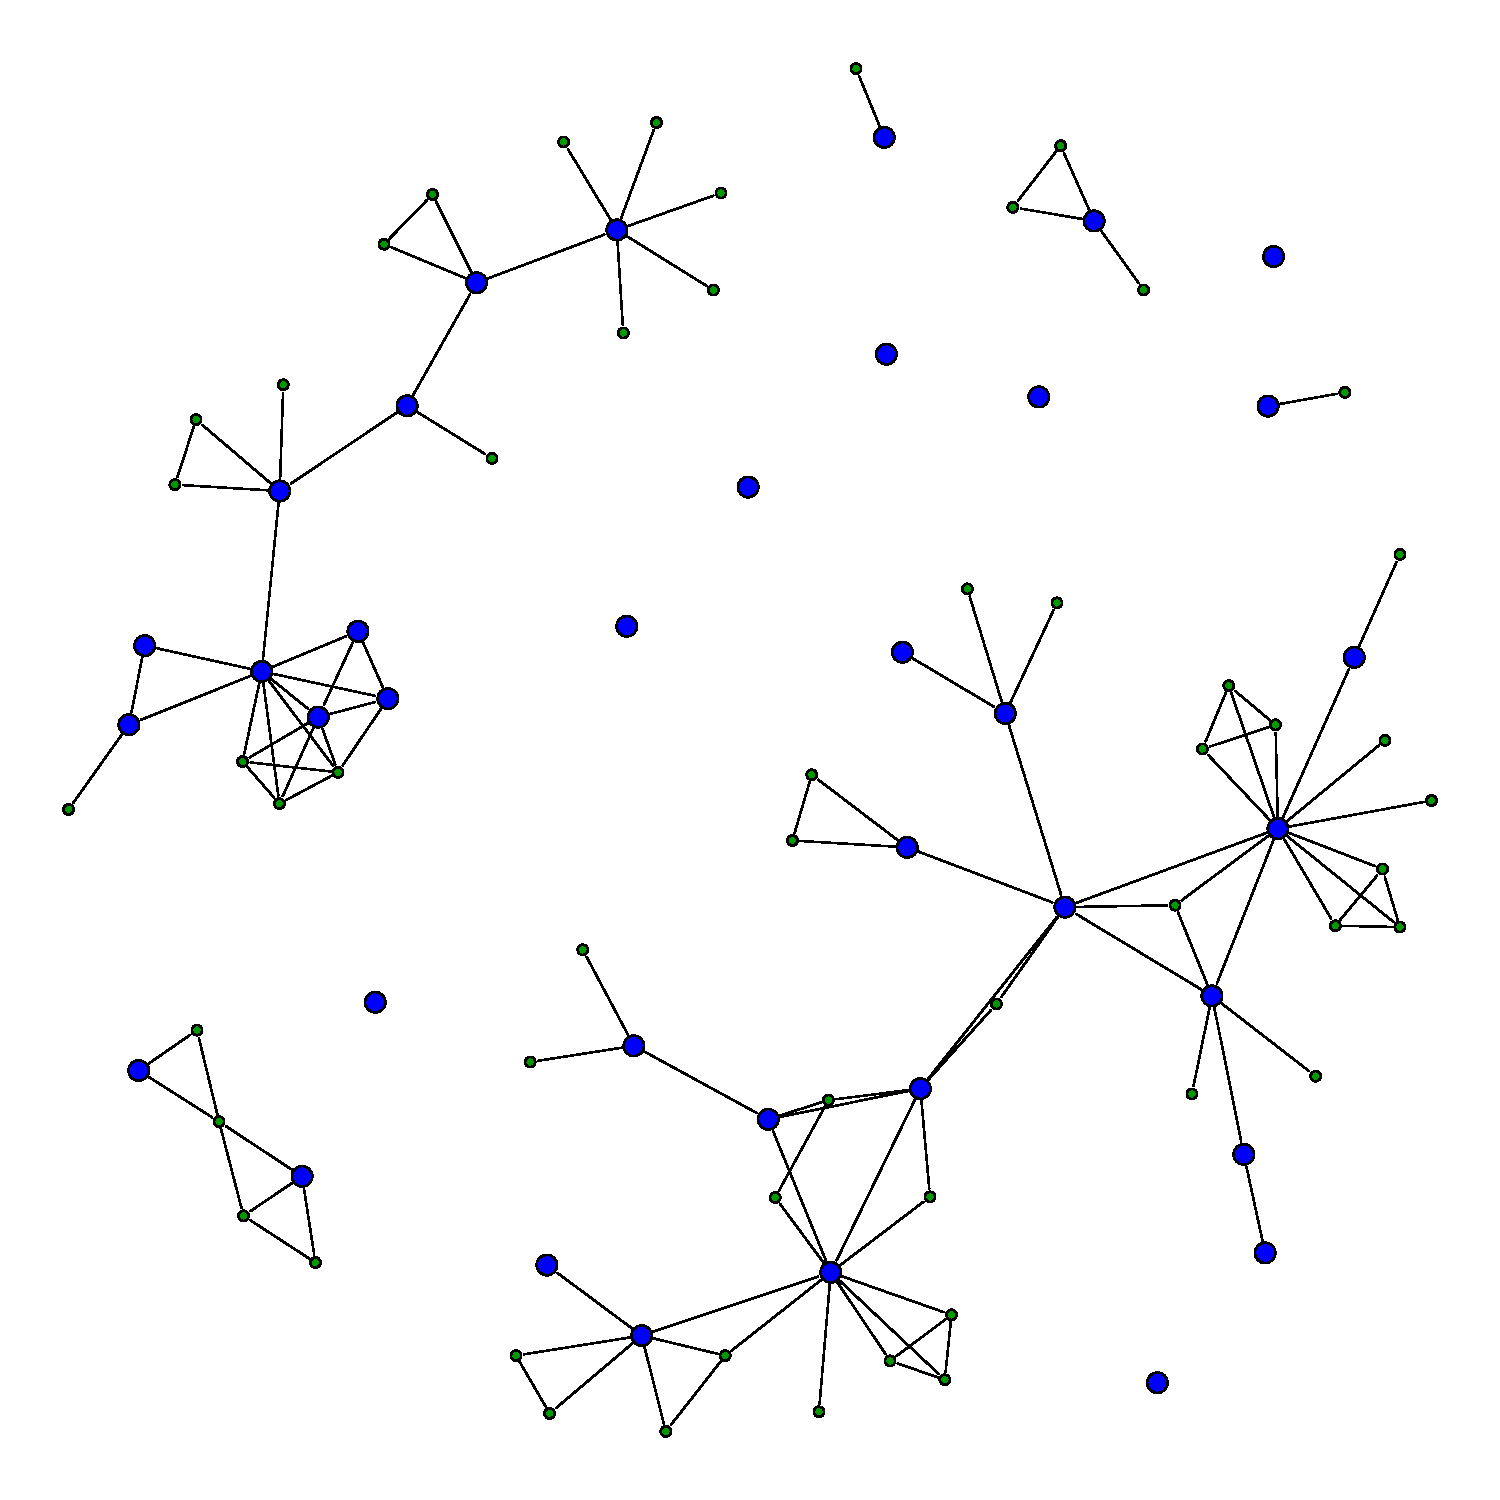
\includegraphics[width=.6\textwidth]{graph}
  \caption{Exemplo de grafo simples.}
  \label{fig:humanbeta}
\end{figure}

\begin{figure}
  \centering
  \begin{subfigure}{0.4\textwidth}
    \centering
    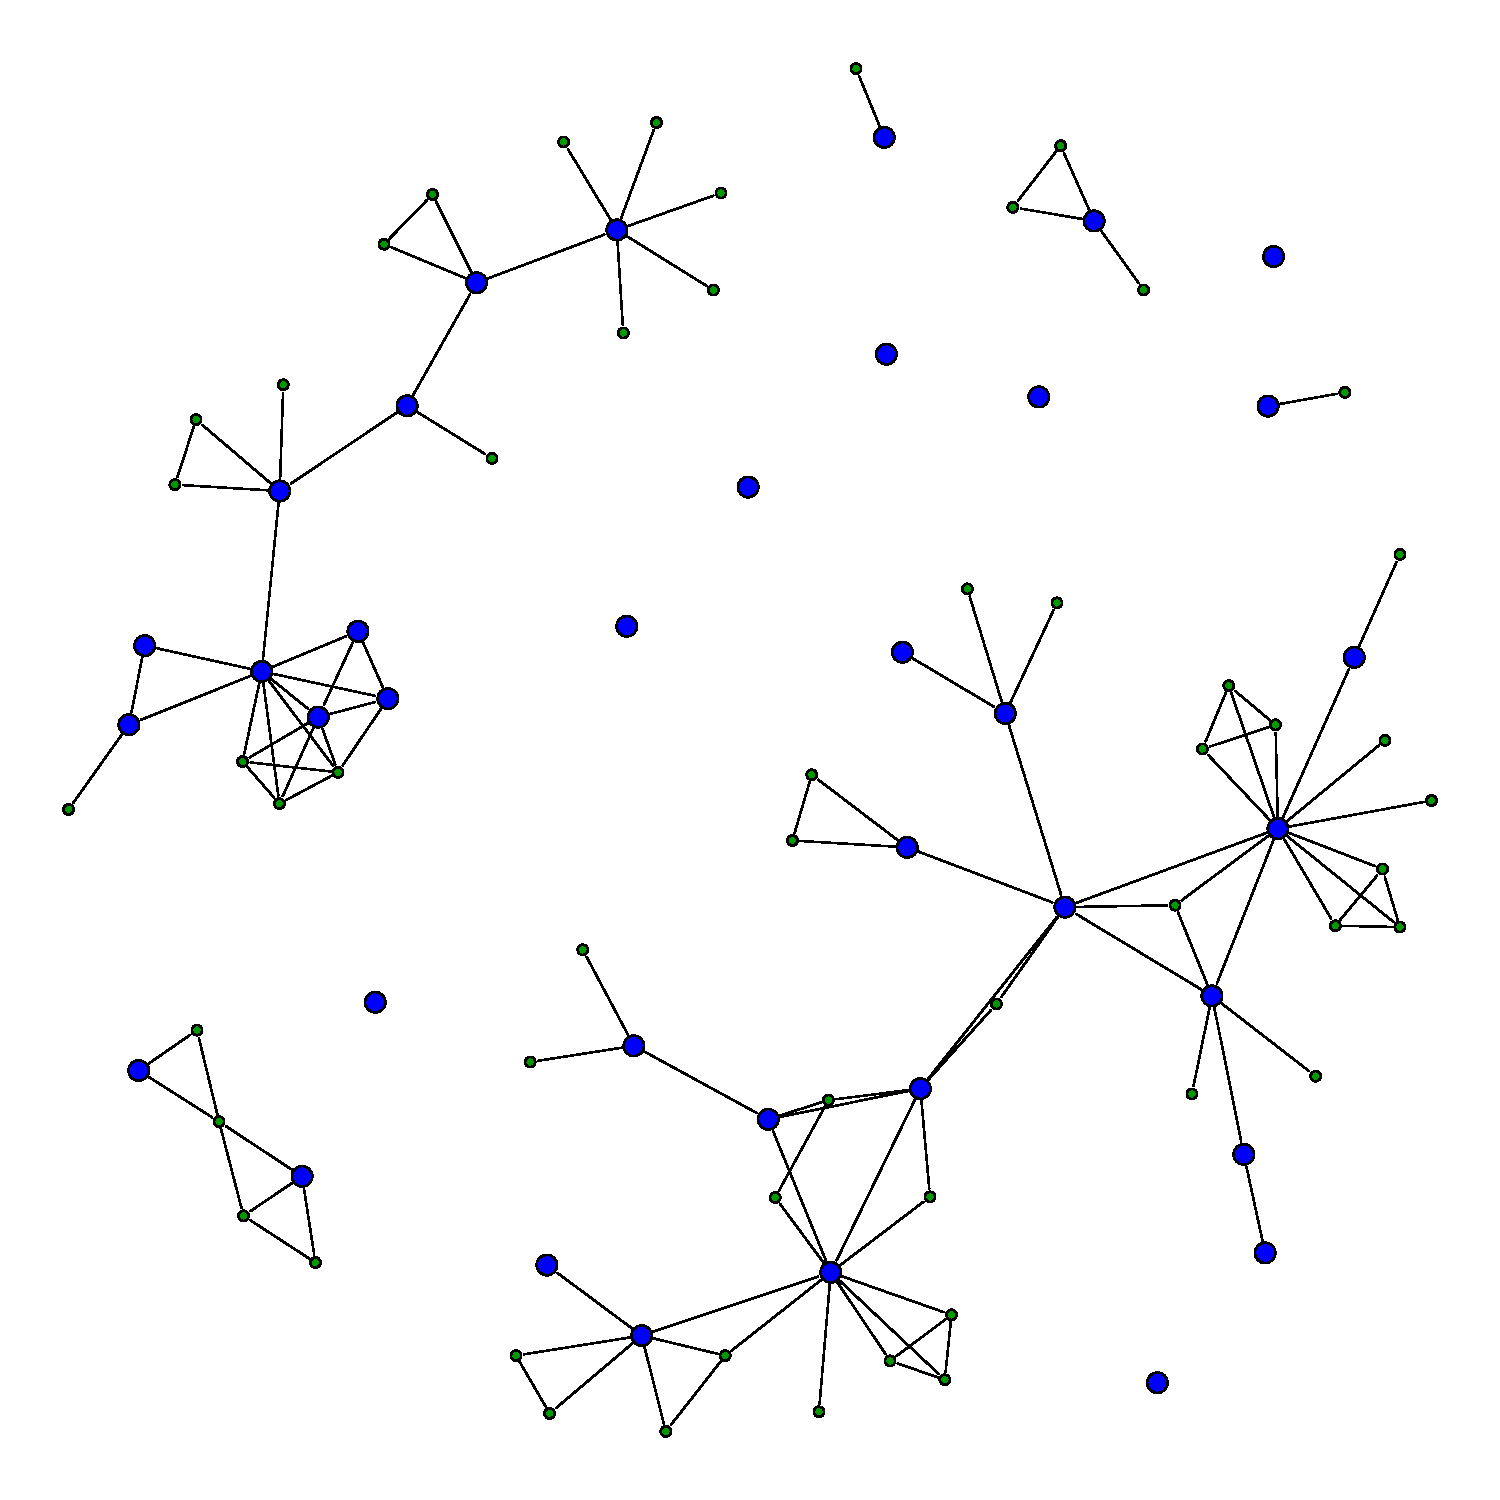
\includegraphics[width=.7\textwidth]{graph}
    \caption{O mesmo exemplo.}
    \label{fig:subfigures:a}
  \end{subfigure}
  \begin{subfigure}{0.4\textwidth}
    \centering
    \begin{turn}{90}
      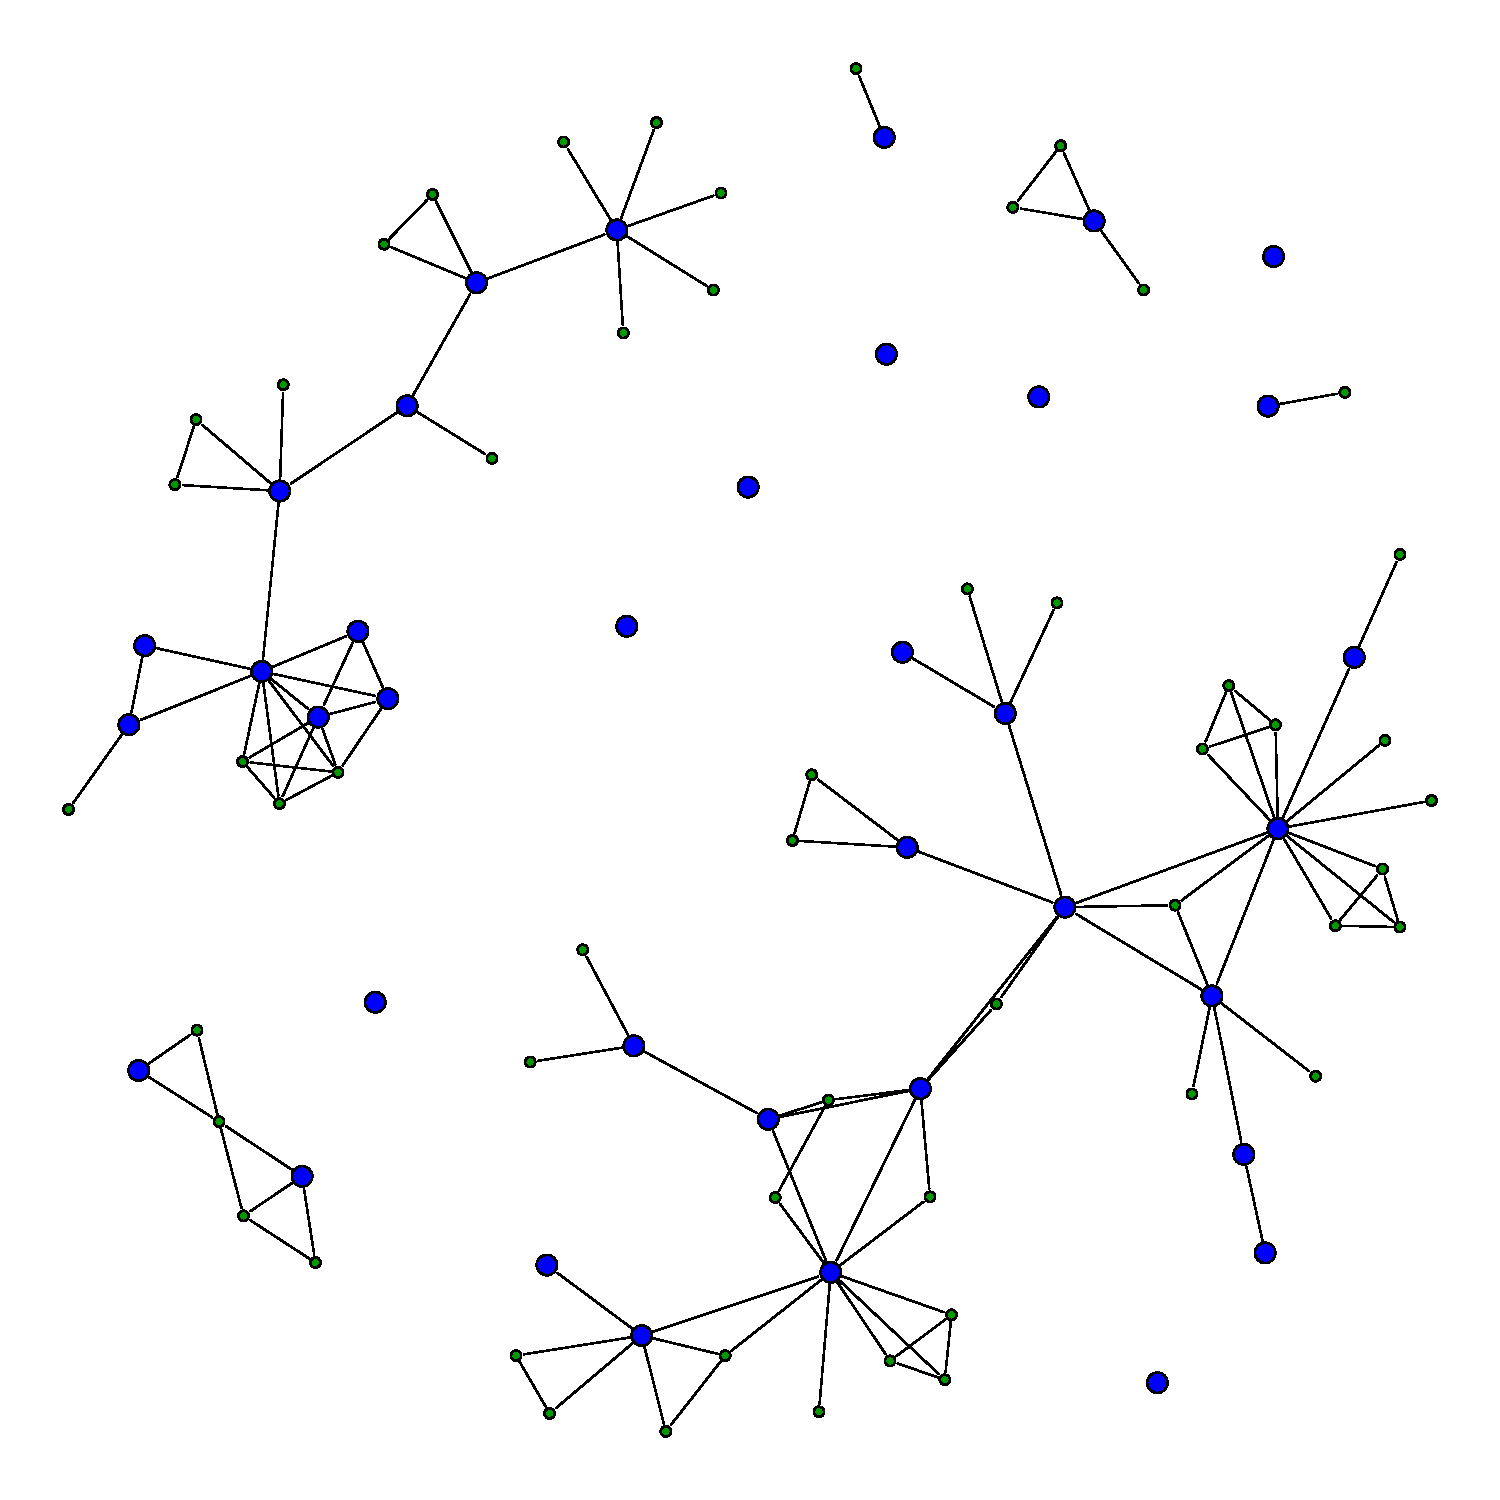
\includegraphics[width=.7\textwidth]{graph}
    \end{turn}
    \caption{O mesmo exemplo, girado.}
    \label{fig:subfigures:b}
  \end{subfigure}
  \caption{Exemplo de subfiguras.}
  \label{fig:subfigures}
\end{figure}


% Foi utilizado o pacote listings para formatar o código fonte
% Veja no preambulo do arquivo tese-exemplo.tex os parâmetros de configuração.
\begin{figure}
  \index{Java}
  \centering
\begin{lstlisting}[language=Java, style=wider]
for (i = 0; i < 20; i++)
{
	// Comentário
	System.out.println("Mensagem...");
}
\end{lstlisting}
  \caption{Exemplo de laço em Java.}
  \label{fig:java}
\end{figure}

Talvez você precise organizar a apresentação da informação na forma de
tabelas\index{Floats}. Há diversos estilos de tabela; um exemplo simples é a
Tabela~\ref{tab:amino_acidos}. A Tabela~\ref{tab:ficha} mostra como construir
uma tabela em forma de ficha larga que deve ser impressa em modo paisagem (ela
é um \textit{float}, mas sempre é impressa em uma página separada). Outro
exemplo de tabela em modo paisagem, esta distribuída em duas páginas (sem ser
um \textit{float}), está no Apêndice \ref{ape:sequencias}\footnote{
Observe que o nome do Apêndice (``\ref{ape:sequencias}'') foi impresso em uma
linha separada, o que não é muito bom visualmente. Para evitar que isso
aconteça (não só no final do parágrafo, mas em qualquer quebra de linha),
faça o que já foi discutido na Seção~\ref{orphanchar} sobre símbolos
matemáticos: utilize um espaço não-separável para fazer referências a
figuras, tabelas, seções etc.: ``\textsf{... está no
Apêndice\textasciitilde\textbackslash{}ref\{ape:sequencias\}}''.}.

\begin{table}
\centering
  \hspace*{\fill}
  \begin{subtable}[b]{0.42\textwidth}
    \centering
    \begin{tabular}{ccl}
      \toprule
      Código & Abreviatura & \makecell{Nome\\completo} \\
      \midrule
      \texttt{A}      & Ala                   & Alanina \\
      \texttt{C}      & Cys                   & Cisteína \\
      ...             & ...                   & ... \\
      \texttt{W}      & Trp                   & Triptofano \\
      \texttt{Y}      & Tyr                   & Tirosina \\
      \bottomrule
    \end{tabular}
    \caption{Uma tabela simples.}
  \end{subtable}
  \hspace*{\fill}\hspace*{\fill}\hspace*{\fill}
  \begin{subtable}[b]{0.37\textwidth}
    \centering
    \begin{tabular}{ccl}
      \rothead{Código} & \rothead{Abreviatura} & \rothead{Nome\\completo} \\
      \midrule
      \texttt{A}      & Ala                   & Alanina \\
      \texttt{C}      & Cys                   & Cisteína \\
      ...             & ...                   & ... \\
      \texttt{W}      & Trp                   & Triptofano \\
      \texttt{Y}      & Tyr                   & Tirosina \\
      \bottomrule
    \end{tabular}
    \caption{Com cabeçalhos girados.}
  \end{subtable}
  \hspace*{\fill}
  \caption{Códigos, abreviaturas e nomes dos aminoácidos.}
  \label{tab:amino_acidos}
\end{table}

% Aumenta o espaçamento entre as linhas da tabela (default: 0pt)
\setlength\extrarowheight{4pt}

% sidewaystable e comandos relacionados são definidos na package rotating
\begin{sidewaystable}
\centering
\begin{tabular}{|M{0.265}|M{0.073}|M{0.084}|M{0.073}|M{0.073}|M{0.08}|M{0.082}|M{0.067}|}
  \hline
    \textbf{Experimento número:} & \multicolumn{2}{c|}{1} & \multicolumn{4}{c|}{\textbf{Data:}} & jan 2017
  \tabularnewline \hline
    \textbf{Título:} & \multicolumn{7}{c|}{Medições iniciais}
  \tabularnewline \hline
    \textbf{Tipo de experimento:} & \multicolumn{7}{c|}{Levantamento quantitativo}
  \tabularnewline \hline \hline
    \textbf{Locais}          & São Paulo & Rio de Janeiro & Porto Alegre & Recife & Manaus & Brasília & Rio Branco
  \tabularnewline \thickhline
    \textbf{Valores obtidos} & 0.2       & 0.3            & 0.2          & 0.7    & 0.5    & 0.1      & 0.4
  \tabularnewline \hline
\end{tabular}
\caption{Exemplo de tabela similar a uma ficha.}
\label{tab:ficha}
\end{sidewaystable}

% Redefinindo para o valor default
\setlength\extrarowheight{0pt}

%\par

%%% ------------------------------------------------------------------------- %%
\chapter{Conclusões}
\label{cap:conclusoes}

Vale muito a pena a leitura do trabalho de
%Uri Alon \cite{alon09:how}, % usando o estilo alpha
Uri \citet{alon09:how}, % usando o estilo plainnat
no qual apresenta-se
uma reflexão sobre a utilização da Lei de Pareto para tentar definir/escolher
problemas para as diferentes fases da vida acadêmica.  A direção dos novos
passos para a continuidade da vida acadêmica deveriam ser discutidos com seu
orientador.

%\par

\par


%%%%%%%%%%%%%%%%%%%%%%%%%%%%%%%% APÊNDICES %%%%%%%%%%%%%%%%%%%%%%%%%%%%%%%%%%%%%

% Aqui vão apêndices. O comando appendix reinicia a numeração de capítulos e
% passa a numerá-los com letras. Como os anteriores, ele não existe na classe
% "article".
%\appendix

%\input{apendices}
%\par


%%%%%%%%%%%%%%%%%%%%%%%%%%%%%% SEÇÕES FINAIS %%%%%%%%%%%%%%%%%%%%%%%%%%%%%%%%%%%

% Aqui vão a bibliografia, índice remissivo e outras seções similares.
% O comando backmatter desabilita a numeração de capítulos e também não existe
% na classe "article".
\backmatter

% Este formato está definido mais acima na seção "APARÊNCIA/FORMATAÇÃO"
\pagestyle{frontback}

\singlespacing   % espaçamento simples

% A bibliografia é obrigatória

%%%%%%%%% Bibliografia com natbib (preterido): %%%%%%%%%
%\bibliographystyle{alpha-ime}% citação bibliográfica alpha
%\bibliographystyle{plainnat-ime} % citação bibliográfica textual
%\bibliography{bibliografia}  % associado ao arquivo: 'bibliografia.bib'

%%%%%%%% Bibliografia com biblatex (preferido): %%%%%%%%

\printbibliography[
  title=Bibliografia\label{bibliografia},
  % Inclui a bibliografia no sumário; comente se estiver usando "article"
  heading=bibintoc,
]

% imprime o índice remissivo no documento (opcional)
\printindex

\end{document}
